% This is the file named 'DSP.tex'
% @LaTeX-file{
% author = {William DeMeo},
% filename = {'DSP.tex'}
% date = {2004/01/08},
% text = {main latex file for collection DSP research paper inputs}
% }


% As per Reed's instructions:
\documentclass[10pt, twocolumn, twoside]{IEEEtran}

%
%%
%%% >>-- BEGIN: MY DEFS --<<
%%
%
\usepackage{amsmath, amssymb, wasysym}
\usepackage{color,times}
%%
%% This is file `wjd.def'
%%
%%% ====================================================================
%%% @LaTeX-file{
%%%   filename  = "wjd.def",
%%%   version   = "0.03.09.08",
%%%   date      = "2003/09/08",
%%%   author    = "William DeMeo",
%%%   email     = "williamdemeo@yahoo.com"
%%% }
%%% ====================================================================
%% 
% -------------------------------------------------------------
% Custom Math Definitions 
% -------------------------------------
%  Algebra & Analysis:
   \newcommand{\field}[1]{\ensuremath{\mathbb{#1}}}
   \newcommand{\Z}{\field{Z}}                   % integers
   \newcommand{\Q}{\field{Q}}                   % rational numbers
   \newcommand{\N}{\field{N}}                   % natural numbers
   \def\R{\field{R}}                   % real numbers 
   \newcommand{\Rn}{\ensuremath{\field{R}^n}}                % the set of n-tuples with elements in \R
   \newcommand{\C}{\field{C}}                   % complex numbers 
   \newcommand{\Cn}{\ensuremath{\field{C}^n}}                % the set of n-tuples with elements in \C
   \newcommand{\rel}{\ensuremath{\mathcal{R}}}                % a general relation
   \newcommand{\Gplus}{\ensuremath{\langle G, + \rangle}}  % a group with binary op \cdot
   \newcommand{\Gdot}{\ensuremath{\langle G, \cdot \rangle}}   % a group with binary op \cdot
   \newcommand{\Group}{\ensuremath{\langle G, * \rangle}}      % a group with binary op *
   \newcommand{\Ring}{\ensuremath{\langle R, +, \cdot \rangle}} % a ring
   \newcommand{\F}{\field{F}}                   % a field
   \newcommand{\Fn}{\ensuremath{\field{F}^n}}                % the set of n-tuples with elements in \F
   \newcommand{\FN}{\ensuremath{\field{F}^N}}                % the set of N-tuples with elements in \F
   \newcommand{\ztwo}{\ensuremath{\field{Z}_2}}              % Cyclic groups (rings)
   \newcommand{\zthree}{\ensuremath{\field{Z}_3}}
   \newcommand{\zfour}{\ensuremath{\field{Z}_4}}
   \newcommand{\Real}{\mbox{Re}} % real part of a complex number  ALT: \newcommand{\Real{\Re}
   \newcommand{\Imag}{\mbox{Im}}
   \newcommand{\integral}{\ensuremath{\int_{-\infty}^{\infty}}}% integration ALT: \newcommand{\integral{\int_{-\infty}^{+\infty}} 

%  Operator Theory and Vector Spaces
   \newcommand{\pv}{\ensuremath{\operatorname{pv}}}
   \newcommand{\W}{\ensuremath{\operatorname{W}}}       % an operator (\eg Wigner-Ville transform)
   \newcommand{\Per}{\ensuremath{\operatorname{Per}}}   % a periodizing operator

   %linear transformations \lt should be sans-serif
   \newcommand{\lt}[1]{\ensuremath{\mathsf{#1}}}
   \newcommand{\ltb}[1]{\ensuremath{[\mathsf{#1}]}}
   \newcommand{\linmap}[3]{\ensuremath{\lt{#1}: \vs{#2} \rightarrow \vs{#3}}}
   \renewcommand{\S}{\lt{S}}       % a linear operator (\eg translation)
   \newcommand{\T}{\lt{T}}       % a linear operator (\eg translation)
   \newcommand{\eye}{\lt{I}}     % the identity operator
   \newcommand{\eyeb}{[\,\lt{I}\,]}     % the identity operator

   % vector spaces should appear in mathcal font.
   \newcommand{\vs}[1]{\ensuremath{\mathcal{#1}}}
   \newcommand{\Lp}{\ensuremath{L^p}}%\newcommand{\Lone}{\vs{L}^1}
   \newcommand{\Linfty}{\ensuremath{L^\infty}}%\newcommand{\Lone}{\vs{L}^1}
   \newcommand{\Lone}{\ensuremath{L^1}}%\newcommand{\Lone}{\vs{L}^1}
   \newcommand{\Ltwo}{\ensuremath{L^2}}%\newcommand{\Ltwo}{\vs{L}^2}
   \newcommand{\ltwo}{\ensuremath{\ell^2}}
   \newcommand{\LpR}{\Lp(\R)}
   \newcommand{\LoneR}{\Lone(\R)}
   \newcommand{\LtwoR}{\Ltwo(\R)}
   \newcommand{\ltwoR}{\ltwo(\R)}
   \newcommand{\LA}{\vs{L}(A)}        % the collection of complex valued functions of $A$.
   \newcommand{\LG}{\vs{L}(G)}        % the collection of complex valued functions of $G$.
   \newcommand{\LZN}{\vs{L}(\Z/N)}    % the collection of complex valued functions of $\Z/N$.
   \newcommand{\Hilbert}{\vs{H}}      % a Hilbert space
   \newcommand{\Banach}{\vs{B}}       % a Banach space
   %   \newcommand{\BanachHH}{\Banach(\Hilbert,\Hilbert)}   % a Banach space
   \newcommand{\Hone}{\vs{H}_1}
   \newcommand{\Htwo}{\vs{H}_2}
   %   \newcommand{\BanachHoneHtwo}{\vs{B}(\Hone,\Htwo)}}
   %   \newcommand{\BanachHtwoHone}{\vs{B}(\Htwo,\Hone)}}
   \newcommand{\esssup}[1]{\ensuremath{\text{ess}\sup_{#1}}}

% old:   
%   \newcommand{\T}{\ensuremath{\operatorname{T}}}
%   \newcommand{\Hilbert}{\ensuremath{\mathcal{H}}}      % a Hilbert space
%   \newcommand{\Hone}{\ensuremath{\mathcal{H}_1}}
%   \newcommand{\Htwo}{\ensuremath{\mathcal{H}_2}}
%   \newcommand{\Banach}{\ensuremath{\mathcal{B}(\Hilbert,\Hilbert)}}   % a Banach space
%   \newcommand{\Banachonetwo}{\ensuremath{\mathcal{B}(\Hone,\Htwo)}}
%   \newcommand{\Banachtwoone}{\ensuremath{\mathcal{B}(\Htwo,\Hone)}}


   \newcommand{\ga}[1]{\ensuremath{\C #1}} %  group algebras
   \newcommand{\CA}{\ga{A}}                % the group algebra of $A$
   \newcommand{\CG}{\ga{G}}                % the group algebra of $G$
   \newcommand{\basis}{\ensuremath{\mathcal{B}}}     % basis
   \newcommand{\Span}{\ensuremath{\mbox{span}}}
   \newcommand{\Null}{\ensuremath{\mathcal{N}}}      % null space
   \newcommand{\Range}{\ensuremath{\mathcal{R}}}     % range
   \newcommand{\Krylov}{\ensuremath{\mathcal{K}}}    
   \newcommand{\FT}{\ensuremath{\mathcal{F}}}    % fourier transform
   \newcommand{\invFT}{\ensuremath{\mathcal{F}^{-1}}} % inverse fourier transform
   \newcommand{\Poi}{\ensuremath{\operatorname{Poi}}}   % Poisson distribution

% The following definition was for manual bolding of vectors:
%   \newcommand{\bx}{\ensuremath{\mathbf{x}}}
% It is ugly and deprecated; better to use the \vec command; e.g. \vec{x}  
%   @ifundefined{vec}{\newcommand{\vec}[1]{\mathbf{#1}}}{}
%   \newcommand{\vec}[1]{\mathbf{#1}}

   \newcommand{\mean}[1]{\overline{#1}} % sample mean of x
% should now use \mean{x} instead of:
%   \newcommand{\sm}{\ensuremath{\overline{x}}}    % sample mean of x
   \newcommand{\Prob}{\field{P}}                      % a probability distribution

% Latin (see LaTeX Companion, p. 50)
   \newcommand{\eg}{e.g.,\space}            % for example (latin: {\it exempli gratia})
   \newcommand{\ie}{i.e.,\space}            % that is     (latin: {\it id est})
   \newcommand{\etc}{etc.\@\space}          % etcetera    (latin: {\it et cetera})
\newcommand{\dotcup}{\ensuremath{\mathaccent\cdot\cup}}

\newcommand\defeq{\ensuremath{\stackrel{\text{def}}{=}}}
\newcommand\net{\ensuremath{\{x_\alpha\}}}
\newcommand\Net{\ensuremath{\{x_\alpha : \alpha \in A\}}}
\newcommand\Netn{\ensuremath{\{x_\alpha : \alpha \in A_n\}}}
\newcommand\rsum{\ensuremath{R(f,P,c)}}
\newcommand\intab{\ensuremath{\int_a^b}}
\newcommand\unsolved{\textcolor{red}{\it Have yet to solve this one!}}
\newcommand\onlyif{\ensuremath{\quad \Rightarrow \quad}}
\newcommand\iif{\ensuremath{\quad \Leftrightarrow \quad}}

\newcommand{\inverse}[1]{\ensuremath{#1^{-1}}}
\newcommand{\inv}[1]{\ensuremath{#1^{-1}}}
\newcommand{\transpose}[1]{\ensuremath{#1^{\lt{t}}}}
\newcommand{\compl}[1]{\ensuremath{#1^{\complement}}}
\newcommand{\smallfrac}[2]{\ensuremath{{\scriptstyle \frac{#1}{#2}}}}
\newcommand{\Clifford}[2]{\ensuremath{\mathcal{C\ell}_{#1,#2}}}

% Memorandum meta data fields
\newcommand{\memometa}[2]{\underline{{\sc {\bf #1:}}}\; #2\\\\}
\newcommand{\memohead}[1]{\lhead{{\sc Textron} Systems}\chead{{\sc Memorandum}}\rhead{#1}}
%\newcommand{\memosec}[1]{\noindent\underline{\bf #1}}
\newcommand{\memosec}[1]{\begin{center}\noindent {\bf #1}\end{center}}

\newcommand{\given}{\ensuremath{\,|\,}}
%\newcommand{\indicator}[1]{\ensuremath{\vec{1}(#1)}}
\newcommand{\vA}{\ensuremath{\vec{A}}}
\newcommand{\vU}{\ensuremath{\vec{U}}}
\newcommand{\Uperp}{\ensuremath{\vec{U}_\perp}}
\newcommand{\Upara}{\ensuremath{\vec{U}_\parallel}}
\newcommand{\Uparaa}{\ensuremath{\vec{U}_{\va}}}
\newcommand{\uperp}{\ensuremath{\vec{u}_\perp}}
\newcommand{\upara}{\ensuremath{\vec{u}_\parallel}}
\newcommand{\vperp}{\ensuremath{\vec{v}_\perp}}
\newcommand{\vpara}{\ensuremath{\vec{v}_\parallel}}

\newcommand\eone{\ensuremath{\vec{e}_1}}
\newcommand\etwo{\ensuremath{\vec{e}_2}}
\newcommand\ethree{\ensuremath{\vec{e}_3}}
\newcommand\Itwo{\ensuremath{\vec{I}_2}}
\newcommand\ITWO{\ensuremath{\eone \wedge \etwo}}
\newcommand\Ithree{\ensuremath{\vec{I}_3}}
\newcommand\ITHREE{\ensuremath{\eone \wedge \etwo \wedge \ethree}}
\newcommand\carrot{\ensuremath{\wedge}}
\newcommand\dual{\text{dual}}
\newcommand\va{\ensuremath{\vec{a}}}
\newcommand\vb{\ensuremath{\vec{b}}}
\newcommand\vB{\ensuremath{\vec{B}}}
\newcommand\vc{\ensuremath{\vec{c}}}
\newcommand\vY{\ensuremath{\vec{Y}}}
\newcommand\vw{\ensuremath{\vec{x}}}
\newcommand\vu{\ensuremath{\vec{u}}}
\newcommand\vv{\ensuremath{\vec{v}}}
\newcommand\vx{\ensuremath{\vec{x}}}
\newcommand\vy{\ensuremath{\vec{y}}}
\newcommand\vz{\ensuremath{\vec{z}}}
\newcommand\indicator[1]{\ensuremath{\vec{1}\{#1\}}}

% might use \startcodebox{12}
\newcommand{\startcodebox}[1]{\begin{center}\setlength{\fboxsep}{4mm}\begin{boxedminipage}[t]{#1cm}}
\newcommand\stopcodebox{\end{boxedminipage}\end{center}\vspace{2mm}}

%--- begin 2004.11.01 additions ---
%\newcommand\UCB{U.~C.~Berkeley}
\newcommand{\school}[1]{{\large{\itshape{#1}}}}
\newcommand{\inst}[1]{{\large{\itshape{#1}}}}
\newcommand{\job}[1]{{\small{\bfseries\sffamily{#1}}}}
\newcommand\hsptwo{}
\newcommand\adjsl{\small  \vspace*{-10pt}}  
\newcommand\brr{\begin{raggedright}}
\newcommand\err{\end{raggedright}}
\newcommand\smallsep{\setlength{\itemsep}{-1pt}}
\newcommand\bigsep{\setlength{\itemsep}{+1pt}}
\newcommand\Yj{\ensuremath{Y_j}}
\newcommand\Xij{\ensuremath{X(i,j)}}
\newcommand{\bi}{\begin{itemize}} 
\newcommand{\ei}{\end{itemize}} 
\newcommand{\bis}{\begin{itemstep}} 
\newcommand{\eis}{\end{itemstep}} 
\newcommand\yields{\ensuremath{\leadsto \;}} 
%--- end 2004.11.01 additions ---

\newcommand\e{\mathrm{e}}    % exponential
   \newcommand\A{\operatorname{A}}
%   \newcommand\E{\operatorname{E}}   % prefer to use \E for e = 3.14...
   \renewcommand\H{\operatorname{H}}
%   \newcommand\I{\operatorname{I}}   % prefer to use \I for imaginary number
   \newcommand\Banachonetwo{\mathcal{B}(\Hone,\Htwo)}
   \newcommand\Banachtwoone{\mathcal{B}(\Htwo,\Hone)}
% Signals, Time-Frequency shifts, etc.
   \newcommand\scale{\frac{1}{\sqrt{s}}}
   \newcommand\transcale{\left(\frac{t-u}{s}\right)}
   \newcommand\xpull{x_{\frac{\tau}{2}, -\frac{\xi}{2}}}
   \newcommand\xpush{x_{-\frac{\tau}{2}, \frac{\xi}{2}}}
   \newcommand\xpullpush{x_{\frac{\tau}{2}, \frac{\xi}{2}}}
   \newcommand\xpushpull{x_{-\frac{\tau}{2}, -\frac{\xi}{2}}}
   \newcommand\xfpull{x_{-\frac{\Delta\nu}{2}}}
   \newcommand\xfpush{x_{\frac{\Delta\nu}{2}}}
   \newcommand\apull{a_{-}}
   \newcommand\apush{a_{+}}
   \newcommand\ytnu{y_{t,\nu}}
   \newcommand\ytnut{\tilde{y}_{t,\nu}}
   \newcommand\half{{\scriptstyle \frac{1}{2}}}
   \newcommand\halftau{{\scriptstyle \frac{\tau}{2}}}
   \newcommand\halfxi{{\scriptstyle \frac{\xi}{2}}}
   \newcommand\halfnu{{\scriptstyle \frac{\nu}{2}}}
   \newcommand\halfDnu{{\scriptstyle \frac{\Delta\nu}{2}}}
   \newcommand\xtpull{x\left(t+\halftau\right)}
   \newcommand\xtpush{x\left(t-\halftau\right)}
%   (shouldn't need this) \newcommand\xtpullconj{x^*\left(t+\halftau\right)}
   \newcommand\xtpushconj{x^*\left(t-\halftau\right)}
   \newcommand\Xtpull{X\left(\nu+\halfxi\right)}
   \newcommand\Xtpush{X\left(\nu-\halfxi\right)}
   \newcommand\Xtpullconj{X^*\left(\nu+\halfxi\right)}
%   (shouldn't need this) \newcommand\Xtpushconj{X^*\left(\nu-\halfxi\right)}

   \newcommand\ytpull{y\left(t+\halftau\right)}
   \newcommand\ytpush{y\left(t-\halftau\right)}
%   (shouldn't need this) \newcommand\ytpullconj{y^*\left(t+\halftau\right)}
   \newcommand\ytpushconj{y^*\left(t-\halftau\right)}
   \newcommand\Ytpull{Y\left(\nu+\halfxi\right)}
   \newcommand\Ytpush{Y\left(\nu-\halfxi\right)}
   \newcommand\Ytpullconj{Y^*\left(\nu+\halfxi\right)}
%   (shouldn't need this) \newcommand\Ytpushconj{Y^*\left(\nu-\halfxi\right)}

% Language
%   \newcommand\FT{Fourier transform}
   \newcommand\WT{Wigner transform}
   \newcommand\WV{Wigner-Ville}


%% Customized section style commands

   \newcommand{\wjdsecstyle}{\scshape\boldmath}
   \newcommand{\wjdsubsecstyle}{\scshape\boldmath}

%     \newcommand\wjdsec[1]{\chapter{\normalfont\wjdsecstyle #1}}
%     \newcommand\wjdsec[1]{\chapter{#1}}
     \newcommand\wjdsec[1]{\section{#1}}
     \newcommand\wjdsubsec[1]{\subsection{#1}}
     \newcommand\wjdsubsubsec[1]{\subsubsection{#1}}
%     \newcommand\wjdparasec[1]{\paragraph{#1}}
     \newcommand\wjdparasec[1]{\subsubsection{#1}}
     \newcommand\wjdappsec[1]{\section{#1}}
     \newcommand\wjdappsubsec[1]{\subsection{#1}}
%     \newcommand\wjdappsubsubsec[1]{\paragraph{#1}}
     \newcommand\wjdappsubsubsec[1]{\subsubsection{#1}}
%     \newcommand\wjdappparasec[1]{\subparagraph{#1}}
     \newcommand\wjdappparasec[1]{\subsubsection{#1}}

     \newcommand\hafgsec[1]{\section{#1}}
     \newcommand\hafgsubsec[1]{\subsection{#1}}
     \newcommand\hafgsubsubsec[1]{\subsubsection{#1}}
     \newcommand\hafgparasec[1]{\paragraph{#1}}

   \newcommand\ismasec[1]{\section{#1}}
   \newcommand\ismasubsec[1]{\subsection{#1}}
   \newcommand\ismasubsubsec[1]{\subsubsection{#1}}
   \newcommand\ismaparasec[1]{\subsubsection{#1}}


   % Binary operator symbols
   \newcommand\sdp{\ensuremath{\varangle}}                      % semi-direct product

   \newcommand\scriptfrac[2]{\ensuremath{{\scriptstyle \frac{#1}{#2}}}}

\newcommand{\functionsec}[1]{\wjdparasec{\hrule\vspace{1mm}\noindent#1}}
\newcommand{\rootxref}[1]{The main function definition begins
  at $\langle${\it #1} \subpageref{root:#1}$\rangle$.}
\newcommand{\shortrootxref}[1]{The main function definition begins
  at chunk~\subpageref{root:#1}.}

\newcommand{\authorref}[1]{{\scshape #1}}

\newcommand{\dotB}{\ensuremath{\dot{\vec{B}}}}
\newcommand{\dotH}{\ensuremath{\dot{\vec{H}}}}
\newcommand{\dotE}{\ensuremath{\dot{\vec{E}}}}
\newcommand{\DdotE}{\ensuremath{\Ddot{\vec{E}}}}
\newcommand{\dotD}{\ensuremath{\dot{\vec{D}}}}
\newcommand{\DdotD}{\ensuremath{\Ddot{\vec{D}}}}

\newcommand{\curl}{\ensuremath{\mathrm{curl\,}}}
\renewcommand{\div}{\ensuremath{\mathrm{div\,}}}
\newcommand{\grad}{\ensuremath{\mathrm{grad\,}}}

% Special notation for exponents and the imaginary number
\newcommand{\E}{\ensuremath{\mathrm{e}}}
\newcommand{\I}{\ensuremath{\mathrm{i}}}

%
% --- Radar and Imaging Definitions ---
%
\newcommand\autocorrelation{\ensuremath{\hat{R}_{\hat{f}\hat{f}}}}
\newcommand\MIf{\ensuremath{\hat{R}_{\hat{f}\hat{f}}}}
\newcommand{\MI}[1]{\ensuremath{\hat{R}_{\hat{#1}\hat{#1}}}}
\newcommand\Pupil{\ensuremath{\vs{P}}}
\newcommand\Focal{\ensuremath{\vs{F}}}
%\newcommand\micro{\ensuremath{\mu}}
\newcommand{\micro}[1]{\ensuremath{\mu\text{#1}}}
\newcommand\km{\ensuremath{\text{km}}}
\newcommand\nmi{\ensuremath{\text{nmi}}}
%\newcommand\Tintrapulse{\ensuremath{\tau_{\text{intrapulse}}}}
\newcommand\pbw{\ensuremath{\tau_{\text{b}}}}  % pulse-burst width
\newcommand\ptw{\ensuremath{\tau_{\text{t}}}}  % pulse-tone width
\newcommand\prp{\ensuremath{T_{\text{p}}}}  % pulse repetition period
\newcommand\prf{\ensuremath{f_{\text{p}}}}  % pulse repetition frequency

\newcommand{\zmv}{\ensuremath{x^m k_v}}
\newcommand{\zmvInv}{\ensuremath{x^{N-wm} k_w}}


% [NB Include file 'wjdthms.def' for end-of-proof symbol]
%\newcommand\qedsymbol{\hbox{\rlap{$\sqcap$}$\sqcup$}}
%\newcommand\qed{\relax\ifmmode\else\unskip\quad\fi\qedsymbol}
%\newcommand\smartqed{\renewcommand\qed{\relax\ifmmode\qedsymbol\else
%  {\unskip\nobreak\hfil\penalty50\hskip1em\null\nobreak\hfil\qedsymbol
%  \parfillskip=\z@\finalhyphendemerits=0\endgraf}\fi}}

%\smartqed

%%-------------------------------------------------------------

\usepackage{theorem}
%%
%% Some theorems not defined by IEEEtran.
%%
{\theorembodyfont{\rmfamily}
 \newtheorem{corollary}{Corollary}
 \newtheorem{example}{Example}
 \newtheorem{theorem}{Theorem}
}
%
%%
%%% >>-- END: MY DEFS --<<
%%
%

%% -- ISMA2004 customizations -------------------------------------------------
%\documentclass[boldvectors]{wjdarticle}
%%\usepackage{icmc}
\usepackage{epsfig}
%\usepackage{fullpage}
%\usepackage{ifthen}
%    %% Should figures be compiled?
%    \newboolean{nofigures}  % initially false ==> compile with figures
%    %\setboolean{nofigures}{true} % un-comment this line to compile without figures
%    \newboolean{nospecialfootnotes}%% Should citation footnotes on section headings be compiled?
%    \setboolean{nospecialfootnotes}{true} % comment this line to compile with special citation foonotes

%\setcounter{page}{1}
%\sloppy         % better line breaks
%%\tenpt
%%SM below a registered trademark definition
%\newcommand\reg{{\rm\ooalign{\hfil
%     \raise.07ex\hbox{\scriptsize R}\hfil\crcr\mathhexbox20D}}}
%% \newcommand{\reg}{\textsuperscript{\textcircled{\textsc r}}}
%%-----------------------------------------------------------------------------


%\usepackage{amsmath,amssymb, wasysym}
%\usepackage{color,boxedminipage,acronym,times}
%%\usepackage{boxedminipage, acronym}
%%\usepackage[pdftex]{color}

%%%
%% This is file `wjd.def'
%%
%%% ====================================================================
%%% @LaTeX-file{
%%%   filename  = "wjd.def",
%%%   version   = "0.03.09.08",
%%%   date      = "2003/09/08",
%%%   author    = "William DeMeo",
%%%   email     = "williamdemeo@yahoo.com"
%%% }
%%% ====================================================================
%% 
% -------------------------------------------------------------
% Custom Math Definitions 
% -------------------------------------
%  Algebra & Analysis:
   \newcommand{\field}[1]{\ensuremath{\mathbb{#1}}}
   \newcommand{\Z}{\field{Z}}                   % integers
   \newcommand{\Q}{\field{Q}}                   % rational numbers
   \newcommand{\N}{\field{N}}                   % natural numbers
   \def\R{\field{R}}                   % real numbers 
   \newcommand{\Rn}{\ensuremath{\field{R}^n}}                % the set of n-tuples with elements in \R
   \newcommand{\C}{\field{C}}                   % complex numbers 
   \newcommand{\Cn}{\ensuremath{\field{C}^n}}                % the set of n-tuples with elements in \C
   \newcommand{\rel}{\ensuremath{\mathcal{R}}}                % a general relation
   \newcommand{\Gplus}{\ensuremath{\langle G, + \rangle}}  % a group with binary op \cdot
   \newcommand{\Gdot}{\ensuremath{\langle G, \cdot \rangle}}   % a group with binary op \cdot
   \newcommand{\Group}{\ensuremath{\langle G, * \rangle}}      % a group with binary op *
   \newcommand{\Ring}{\ensuremath{\langle R, +, \cdot \rangle}} % a ring
   \newcommand{\F}{\field{F}}                   % a field
   \newcommand{\Fn}{\ensuremath{\field{F}^n}}                % the set of n-tuples with elements in \F
   \newcommand{\FN}{\ensuremath{\field{F}^N}}                % the set of N-tuples with elements in \F
   \newcommand{\ztwo}{\ensuremath{\field{Z}_2}}              % Cyclic groups (rings)
   \newcommand{\zthree}{\ensuremath{\field{Z}_3}}
   \newcommand{\zfour}{\ensuremath{\field{Z}_4}}
   \newcommand{\Real}{\mbox{Re}} % real part of a complex number  ALT: \newcommand{\Real{\Re}
   \newcommand{\Imag}{\mbox{Im}}
   \newcommand{\integral}{\ensuremath{\int_{-\infty}^{\infty}}}% integration ALT: \newcommand{\integral{\int_{-\infty}^{+\infty}} 

%  Operator Theory and Vector Spaces
   \newcommand{\pv}{\ensuremath{\operatorname{pv}}}
   \newcommand{\W}{\ensuremath{\operatorname{W}}}       % an operator (\eg Wigner-Ville transform)
   \newcommand{\Per}{\ensuremath{\operatorname{Per}}}   % a periodizing operator

   %linear transformations \lt should be sans-serif
   \newcommand{\lt}[1]{\ensuremath{\mathsf{#1}}}
   \newcommand{\ltb}[1]{\ensuremath{[\mathsf{#1}]}}
   \newcommand{\linmap}[3]{\ensuremath{\lt{#1}: \vs{#2} \rightarrow \vs{#3}}}
   \renewcommand{\S}{\lt{S}}       % a linear operator (\eg translation)
   \newcommand{\T}{\lt{T}}       % a linear operator (\eg translation)
   \newcommand{\eye}{\lt{I}}     % the identity operator
   \newcommand{\eyeb}{[\,\lt{I}\,]}     % the identity operator

   % vector spaces should appear in mathcal font.
   \newcommand{\vs}[1]{\ensuremath{\mathcal{#1}}}
   \newcommand{\Lp}{\ensuremath{L^p}}%\newcommand{\Lone}{\vs{L}^1}
   \newcommand{\Linfty}{\ensuremath{L^\infty}}%\newcommand{\Lone}{\vs{L}^1}
   \newcommand{\Lone}{\ensuremath{L^1}}%\newcommand{\Lone}{\vs{L}^1}
   \newcommand{\Ltwo}{\ensuremath{L^2}}%\newcommand{\Ltwo}{\vs{L}^2}
   \newcommand{\ltwo}{\ensuremath{\ell^2}}
   \newcommand{\LpR}{\Lp(\R)}
   \newcommand{\LoneR}{\Lone(\R)}
   \newcommand{\LtwoR}{\Ltwo(\R)}
   \newcommand{\ltwoR}{\ltwo(\R)}
   \newcommand{\LA}{\vs{L}(A)}        % the collection of complex valued functions of $A$.
   \newcommand{\LG}{\vs{L}(G)}        % the collection of complex valued functions of $G$.
   \newcommand{\LZN}{\vs{L}(\Z/N)}    % the collection of complex valued functions of $\Z/N$.
   \newcommand{\Hilbert}{\vs{H}}      % a Hilbert space
   \newcommand{\Banach}{\vs{B}}       % a Banach space
   %   \newcommand{\BanachHH}{\Banach(\Hilbert,\Hilbert)}   % a Banach space
   \newcommand{\Hone}{\vs{H}_1}
   \newcommand{\Htwo}{\vs{H}_2}
   %   \newcommand{\BanachHoneHtwo}{\vs{B}(\Hone,\Htwo)}}
   %   \newcommand{\BanachHtwoHone}{\vs{B}(\Htwo,\Hone)}}
   \newcommand{\esssup}[1]{\ensuremath{\text{ess}\sup_{#1}}}

% old:   
%   \newcommand{\T}{\ensuremath{\operatorname{T}}}
%   \newcommand{\Hilbert}{\ensuremath{\mathcal{H}}}      % a Hilbert space
%   \newcommand{\Hone}{\ensuremath{\mathcal{H}_1}}
%   \newcommand{\Htwo}{\ensuremath{\mathcal{H}_2}}
%   \newcommand{\Banach}{\ensuremath{\mathcal{B}(\Hilbert,\Hilbert)}}   % a Banach space
%   \newcommand{\Banachonetwo}{\ensuremath{\mathcal{B}(\Hone,\Htwo)}}
%   \newcommand{\Banachtwoone}{\ensuremath{\mathcal{B}(\Htwo,\Hone)}}


   \newcommand{\ga}[1]{\ensuremath{\C #1}} %  group algebras
   \newcommand{\CA}{\ga{A}}                % the group algebra of $A$
   \newcommand{\CG}{\ga{G}}                % the group algebra of $G$
   \newcommand{\basis}{\ensuremath{\mathcal{B}}}     % basis
   \newcommand{\Span}{\ensuremath{\mbox{span}}}
   \newcommand{\Null}{\ensuremath{\mathcal{N}}}      % null space
   \newcommand{\Range}{\ensuremath{\mathcal{R}}}     % range
   \newcommand{\Krylov}{\ensuremath{\mathcal{K}}}    
   \newcommand{\FT}{\ensuremath{\mathcal{F}}}    % fourier transform
   \newcommand{\invFT}{\ensuremath{\mathcal{F}^{-1}}} % inverse fourier transform
   \newcommand{\Poi}{\ensuremath{\operatorname{Poi}}}   % Poisson distribution

% The following definition was for manual bolding of vectors:
%   \newcommand{\bx}{\ensuremath{\mathbf{x}}}
% It is ugly and deprecated; better to use the \vec command; e.g. \vec{x}  
%   @ifundefined{vec}{\newcommand{\vec}[1]{\mathbf{#1}}}{}
%   \newcommand{\vec}[1]{\mathbf{#1}}

   \newcommand{\mean}[1]{\overline{#1}} % sample mean of x
% should now use \mean{x} instead of:
%   \newcommand{\sm}{\ensuremath{\overline{x}}}    % sample mean of x
   \newcommand{\Prob}{\field{P}}                      % a probability distribution

% Latin (see LaTeX Companion, p. 50)
   \newcommand{\eg}{e.g.,\space}            % for example (latin: {\it exempli gratia})
   \newcommand{\ie}{i.e.,\space}            % that is     (latin: {\it id est})
   \newcommand{\etc}{etc.\@\space}          % etcetera    (latin: {\it et cetera})
\newcommand{\dotcup}{\ensuremath{\mathaccent\cdot\cup}}

\newcommand\defeq{\ensuremath{\stackrel{\text{def}}{=}}}
\newcommand\net{\ensuremath{\{x_\alpha\}}}
\newcommand\Net{\ensuremath{\{x_\alpha : \alpha \in A\}}}
\newcommand\Netn{\ensuremath{\{x_\alpha : \alpha \in A_n\}}}
\newcommand\rsum{\ensuremath{R(f,P,c)}}
\newcommand\intab{\ensuremath{\int_a^b}}
\newcommand\unsolved{\textcolor{red}{\it Have yet to solve this one!}}
\newcommand\onlyif{\ensuremath{\quad \Rightarrow \quad}}
\newcommand\iif{\ensuremath{\quad \Leftrightarrow \quad}}

\newcommand{\inverse}[1]{\ensuremath{#1^{-1}}}
\newcommand{\inv}[1]{\ensuremath{#1^{-1}}}
\newcommand{\transpose}[1]{\ensuremath{#1^{\lt{t}}}}
\newcommand{\compl}[1]{\ensuremath{#1^{\complement}}}
\newcommand{\smallfrac}[2]{\ensuremath{{\scriptstyle \frac{#1}{#2}}}}
\newcommand{\Clifford}[2]{\ensuremath{\mathcal{C\ell}_{#1,#2}}}

% Memorandum meta data fields
\newcommand{\memometa}[2]{\underline{{\sc {\bf #1:}}}\; #2\\\\}
\newcommand{\memohead}[1]{\lhead{{\sc Textron} Systems}\chead{{\sc Memorandum}}\rhead{#1}}
%\newcommand{\memosec}[1]{\noindent\underline{\bf #1}}
\newcommand{\memosec}[1]{\begin{center}\noindent {\bf #1}\end{center}}

\newcommand{\given}{\ensuremath{\,|\,}}
%\newcommand{\indicator}[1]{\ensuremath{\vec{1}(#1)}}
\newcommand{\vA}{\ensuremath{\vec{A}}}
\newcommand{\vU}{\ensuremath{\vec{U}}}
\newcommand{\Uperp}{\ensuremath{\vec{U}_\perp}}
\newcommand{\Upara}{\ensuremath{\vec{U}_\parallel}}
\newcommand{\Uparaa}{\ensuremath{\vec{U}_{\va}}}
\newcommand{\uperp}{\ensuremath{\vec{u}_\perp}}
\newcommand{\upara}{\ensuremath{\vec{u}_\parallel}}
\newcommand{\vperp}{\ensuremath{\vec{v}_\perp}}
\newcommand{\vpara}{\ensuremath{\vec{v}_\parallel}}

\newcommand\eone{\ensuremath{\vec{e}_1}}
\newcommand\etwo{\ensuremath{\vec{e}_2}}
\newcommand\ethree{\ensuremath{\vec{e}_3}}
\newcommand\Itwo{\ensuremath{\vec{I}_2}}
\newcommand\ITWO{\ensuremath{\eone \wedge \etwo}}
\newcommand\Ithree{\ensuremath{\vec{I}_3}}
\newcommand\ITHREE{\ensuremath{\eone \wedge \etwo \wedge \ethree}}
\newcommand\carrot{\ensuremath{\wedge}}
\newcommand\dual{\text{dual}}
\newcommand\va{\ensuremath{\vec{a}}}
\newcommand\vb{\ensuremath{\vec{b}}}
\newcommand\vB{\ensuremath{\vec{B}}}
\newcommand\vc{\ensuremath{\vec{c}}}
\newcommand\vY{\ensuremath{\vec{Y}}}
\newcommand\vw{\ensuremath{\vec{x}}}
\newcommand\vu{\ensuremath{\vec{u}}}
\newcommand\vv{\ensuremath{\vec{v}}}
\newcommand\vx{\ensuremath{\vec{x}}}
\newcommand\vy{\ensuremath{\vec{y}}}
\newcommand\vz{\ensuremath{\vec{z}}}
\newcommand\indicator[1]{\ensuremath{\vec{1}\{#1\}}}

% might use \startcodebox{12}
\newcommand{\startcodebox}[1]{\begin{center}\setlength{\fboxsep}{4mm}\begin{boxedminipage}[t]{#1cm}}
\newcommand\stopcodebox{\end{boxedminipage}\end{center}\vspace{2mm}}

%--- begin 2004.11.01 additions ---
%\newcommand\UCB{U.~C.~Berkeley}
\newcommand{\school}[1]{{\large{\itshape{#1}}}}
\newcommand{\inst}[1]{{\large{\itshape{#1}}}}
\newcommand{\job}[1]{{\small{\bfseries\sffamily{#1}}}}
\newcommand\hsptwo{}
\newcommand\adjsl{\small  \vspace*{-10pt}}  
\newcommand\brr{\begin{raggedright}}
\newcommand\err{\end{raggedright}}
\newcommand\smallsep{\setlength{\itemsep}{-1pt}}
\newcommand\bigsep{\setlength{\itemsep}{+1pt}}
\newcommand\Yj{\ensuremath{Y_j}}
\newcommand\Xij{\ensuremath{X(i,j)}}
\newcommand{\bi}{\begin{itemize}} 
\newcommand{\ei}{\end{itemize}} 
\newcommand{\bis}{\begin{itemstep}} 
\newcommand{\eis}{\end{itemstep}} 
\newcommand\yields{\ensuremath{\leadsto \;}} 
%--- end 2004.11.01 additions ---

\newcommand\e{\mathrm{e}}    % exponential
   \newcommand\A{\operatorname{A}}
%   \newcommand\E{\operatorname{E}}   % prefer to use \E for e = 3.14...
   \renewcommand\H{\operatorname{H}}
%   \newcommand\I{\operatorname{I}}   % prefer to use \I for imaginary number
   \newcommand\Banachonetwo{\mathcal{B}(\Hone,\Htwo)}
   \newcommand\Banachtwoone{\mathcal{B}(\Htwo,\Hone)}
% Signals, Time-Frequency shifts, etc.
   \newcommand\scale{\frac{1}{\sqrt{s}}}
   \newcommand\transcale{\left(\frac{t-u}{s}\right)}
   \newcommand\xpull{x_{\frac{\tau}{2}, -\frac{\xi}{2}}}
   \newcommand\xpush{x_{-\frac{\tau}{2}, \frac{\xi}{2}}}
   \newcommand\xpullpush{x_{\frac{\tau}{2}, \frac{\xi}{2}}}
   \newcommand\xpushpull{x_{-\frac{\tau}{2}, -\frac{\xi}{2}}}
   \newcommand\xfpull{x_{-\frac{\Delta\nu}{2}}}
   \newcommand\xfpush{x_{\frac{\Delta\nu}{2}}}
   \newcommand\apull{a_{-}}
   \newcommand\apush{a_{+}}
   \newcommand\ytnu{y_{t,\nu}}
   \newcommand\ytnut{\tilde{y}_{t,\nu}}
   \newcommand\half{{\scriptstyle \frac{1}{2}}}
   \newcommand\halftau{{\scriptstyle \frac{\tau}{2}}}
   \newcommand\halfxi{{\scriptstyle \frac{\xi}{2}}}
   \newcommand\halfnu{{\scriptstyle \frac{\nu}{2}}}
   \newcommand\halfDnu{{\scriptstyle \frac{\Delta\nu}{2}}}
   \newcommand\xtpull{x\left(t+\halftau\right)}
   \newcommand\xtpush{x\left(t-\halftau\right)}
%   (shouldn't need this) \newcommand\xtpullconj{x^*\left(t+\halftau\right)}
   \newcommand\xtpushconj{x^*\left(t-\halftau\right)}
   \newcommand\Xtpull{X\left(\nu+\halfxi\right)}
   \newcommand\Xtpush{X\left(\nu-\halfxi\right)}
   \newcommand\Xtpullconj{X^*\left(\nu+\halfxi\right)}
%   (shouldn't need this) \newcommand\Xtpushconj{X^*\left(\nu-\halfxi\right)}

   \newcommand\ytpull{y\left(t+\halftau\right)}
   \newcommand\ytpush{y\left(t-\halftau\right)}
%   (shouldn't need this) \newcommand\ytpullconj{y^*\left(t+\halftau\right)}
   \newcommand\ytpushconj{y^*\left(t-\halftau\right)}
   \newcommand\Ytpull{Y\left(\nu+\halfxi\right)}
   \newcommand\Ytpush{Y\left(\nu-\halfxi\right)}
   \newcommand\Ytpullconj{Y^*\left(\nu+\halfxi\right)}
%   (shouldn't need this) \newcommand\Ytpushconj{Y^*\left(\nu-\halfxi\right)}

% Language
%   \newcommand\FT{Fourier transform}
   \newcommand\WT{Wigner transform}
   \newcommand\WV{Wigner-Ville}


%% Customized section style commands

   \newcommand{\wjdsecstyle}{\scshape\boldmath}
   \newcommand{\wjdsubsecstyle}{\scshape\boldmath}

%     \newcommand\wjdsec[1]{\chapter{\normalfont\wjdsecstyle #1}}
%     \newcommand\wjdsec[1]{\chapter{#1}}
     \newcommand\wjdsec[1]{\section{#1}}
     \newcommand\wjdsubsec[1]{\subsection{#1}}
     \newcommand\wjdsubsubsec[1]{\subsubsection{#1}}
%     \newcommand\wjdparasec[1]{\paragraph{#1}}
     \newcommand\wjdparasec[1]{\subsubsection{#1}}
     \newcommand\wjdappsec[1]{\section{#1}}
     \newcommand\wjdappsubsec[1]{\subsection{#1}}
%     \newcommand\wjdappsubsubsec[1]{\paragraph{#1}}
     \newcommand\wjdappsubsubsec[1]{\subsubsection{#1}}
%     \newcommand\wjdappparasec[1]{\subparagraph{#1}}
     \newcommand\wjdappparasec[1]{\subsubsection{#1}}

     \newcommand\hafgsec[1]{\section{#1}}
     \newcommand\hafgsubsec[1]{\subsection{#1}}
     \newcommand\hafgsubsubsec[1]{\subsubsection{#1}}
     \newcommand\hafgparasec[1]{\paragraph{#1}}

   \newcommand\ismasec[1]{\section{#1}}
   \newcommand\ismasubsec[1]{\subsection{#1}}
   \newcommand\ismasubsubsec[1]{\subsubsection{#1}}
   \newcommand\ismaparasec[1]{\subsubsection{#1}}


   % Binary operator symbols
   \newcommand\sdp{\ensuremath{\varangle}}                      % semi-direct product

   \newcommand\scriptfrac[2]{\ensuremath{{\scriptstyle \frac{#1}{#2}}}}

\newcommand{\functionsec}[1]{\wjdparasec{\hrule\vspace{1mm}\noindent#1}}
\newcommand{\rootxref}[1]{The main function definition begins
  at $\langle${\it #1} \subpageref{root:#1}$\rangle$.}
\newcommand{\shortrootxref}[1]{The main function definition begins
  at chunk~\subpageref{root:#1}.}

\newcommand{\authorref}[1]{{\scshape #1}}

\newcommand{\dotB}{\ensuremath{\dot{\vec{B}}}}
\newcommand{\dotH}{\ensuremath{\dot{\vec{H}}}}
\newcommand{\dotE}{\ensuremath{\dot{\vec{E}}}}
\newcommand{\DdotE}{\ensuremath{\Ddot{\vec{E}}}}
\newcommand{\dotD}{\ensuremath{\dot{\vec{D}}}}
\newcommand{\DdotD}{\ensuremath{\Ddot{\vec{D}}}}

\newcommand{\curl}{\ensuremath{\mathrm{curl\,}}}
\renewcommand{\div}{\ensuremath{\mathrm{div\,}}}
\newcommand{\grad}{\ensuremath{\mathrm{grad\,}}}

% Special notation for exponents and the imaginary number
\newcommand{\E}{\ensuremath{\mathrm{e}}}
\newcommand{\I}{\ensuremath{\mathrm{i}}}

%
% --- Radar and Imaging Definitions ---
%
\newcommand\autocorrelation{\ensuremath{\hat{R}_{\hat{f}\hat{f}}}}
\newcommand\MIf{\ensuremath{\hat{R}_{\hat{f}\hat{f}}}}
\newcommand{\MI}[1]{\ensuremath{\hat{R}_{\hat{#1}\hat{#1}}}}
\newcommand\Pupil{\ensuremath{\vs{P}}}
\newcommand\Focal{\ensuremath{\vs{F}}}
%\newcommand\micro{\ensuremath{\mu}}
\newcommand{\micro}[1]{\ensuremath{\mu\text{#1}}}
\newcommand\km{\ensuremath{\text{km}}}
\newcommand\nmi{\ensuremath{\text{nmi}}}
%\newcommand\Tintrapulse{\ensuremath{\tau_{\text{intrapulse}}}}
\newcommand\pbw{\ensuremath{\tau_{\text{b}}}}  % pulse-burst width
\newcommand\ptw{\ensuremath{\tau_{\text{t}}}}  % pulse-tone width
\newcommand\prp{\ensuremath{T_{\text{p}}}}  % pulse repetition period
\newcommand\prf{\ensuremath{f_{\text{p}}}}  % pulse repetition frequency

\newcommand{\zmv}{\ensuremath{x^m k_v}}
\newcommand{\zmvInv}{\ensuremath{x^{N-wm} k_w}}


% [NB Include file 'wjdthms.def' for end-of-proof symbol]
%\newcommand\qedsymbol{\hbox{\rlap{$\sqcap$}$\sqcup$}}
%\newcommand\qed{\relax\ifmmode\else\unskip\quad\fi\qedsymbol}
%\newcommand\smartqed{\renewcommand\qed{\relax\ifmmode\qedsymbol\else
%  {\unskip\nobreak\hfil\penalty50\hskip1em\null\nobreak\hfil\qedsymbol
%  \parfillskip=\z@\finalhyphendemerits=0\endgraf}\fi}}

%\smartqed

%%-------------------------------------------------------------

%\input{wjdthms.def}
%%\smartqed
%%%-------------------------------------------------------------

%\title{Topics in Nonabelian Harmonic \\ Analysis and DSP Applications}
\title{Harmonic Analysis on Finite Groups \\ and DSP Applications}

% icmc author command:
%\oneauthor
%{William J.~DeMeo} 
%{Textron Systems Corporation \\ 
%{\small \tt williamdemeo@yahoo.com}}
\author{William J.~DeMeo\\ 
{\small \tt williamdemeo@yahoo.com}}

\begin{document}
% -- ISMA2004 customizations -------------------------------------------------
%  \thispagestyle{isma}
  \maketitle
%-----------------------------------------------------------------------------

%--ABSTRACTS---------------------------------------------------------------------------
\begin{abstract}

%\verb!\input{DSP/isma2004-abstract-short}!
%\input{DSP/isma2004-abstract-short}

%\verb!\input{DSP/isma2004-abstract-long}!
%\input{DSP/isma2004-abstract-long}

\verb!Underlying most digital signal processing (DSP) algorithms
is the group $\Z/N$ of integers modulo $N$, which is
taken as the data indexing set. Translations are defined
using addition modulo $N$, and DSP operations, including
convolutions and Fourier expansions, are then developed
relative to these translations. Recently, An and
Tolimieri~\cite{An:2003} considered a different class of
index set mappings, which arise when the underlying group is
nonabelian, and successfully apply them to 2D image data. 

The present work provides an overview of harmonic analysis on finite
groups and group algebras. 
%I present the basic nonabelian group theory relevant to DSP, and define 
``Generalized translation,'' and its consequence, ``generalized
convolution'' are defined.  Thereafter, some concrete and simple, yet revealing,
examples of nonabelian-group indexing sets  
are discussed along with their practical DSP implications.
%Numerical results are provided along with the
%Matlab source code for reproducing them.
!
Underlying most digital signal processing (DSP) algorithms
is the group $\Z/N$ of integers modulo $N$, which is
taken as the data indexing set. Translations are defined
using addition modulo $N$, and DSP operations, including
convolutions and Fourier expansions, are then developed
relative to these translations. Recently, An and
Tolimieri~\cite{An:2003} considered a different class of
index set mappings, which arise when the underlying group is
nonabelian, and successfully apply them to 2D image data. 

The present work provides an overview of harmonic analysis on finite
groups and group algebras. 
%I present the basic nonabelian group theory relevant to DSP, and define 
``Generalized translation,'' and its consequence, ``generalized
convolution'' are defined.  Thereafter, some concrete and simple, yet revealing,
examples of nonabelian-group indexing sets  
are discussed along with their practical DSP implications.
%Numerical results are provided along with the
%Matlab source code for reproducing them.

\end{abstract}

%--INTROS---------------------------------------------------------------------------
%\verb!\input{DSP/isma2004-intro-short}!
%\input{DSP/isma2004-intro-short}

%\verb!\input{DSP/isma2004-intro-long}!
%\input{DSP/isma2004-intro-long}

\verb!\section{Introduction}
%\PARstart{T}{he} translation-invariance of most classical signal
The translation-invariance of most classical signal
processing transforms and filtering operations is largely
responsible for their widespread use, and is crucial for
efficient algorithmic implementation and interpretation 
of results~\cite{An:2003}. 

DSP on \emph{finite abelian groups} such as $\Z/N$ is
well understood and has great practical utility.  
Translations are defined using addition modulo $N$, and 
basic operations, including convolutions and Fourier 
expansions, are developed relative to these translations~\cite{Tolimieri:1998}. 
%An
%excellent treatment that is applications oriented while
%remaining fairly abstract and general, is provided by 
%%\citeN{Tolimieri:1998}.
%Tolimieri and An in \cite{Tolimieri:1998}.
Recently, however, interest in the practical utility of
\emph{finite nonabelian groups} has grown
significantly. Although the theoretical foundations of
nonabelian groups is well established, application of the
theory to DSP has yet to  become common-place.
%; cf.~the NATO
%ASI ``Computational Non-commutative Algebras,'' Italy,
%2003. Another
A notable exception is~\cite{An:2003},
which develops theory and algorithms for
indexing data with nonabelian groups, defining translations
with a non-commutative group multiply operation, and
performing typical DSP operations relative to these
translations. 
%The work %of An and Tolimieri 
%demonstrates that including nonabelian groups among the
%possible data indexing strategies significantly broadens the
%range of useful signal processing techniques.

This paper describes the use of nonabelian groups
for indexing one- and two-dimensional signals, and discusses 
some computational advantages and insights that can be gained from 
such an approach. 
A simple but instructive class of 
nonabelian groups 
%-- the \emph{semidirect product} groups --
is examined.  When elements of such
groups are used to index the data, and standard DSP
operations are defined with respect to special group
binary operators, more general and interesting
signal transformations are possible.
%=======================================================================
\subsection{Preview: Two Distinctions of Consequence}
Abelian group DSP can be completely described in terms of a
special class of signals called the \emph{characters} of the
group. (For $\Z/N$, the characters are simply the exponentials.)
Each character of an abelian group represents a one-dimensional
translation-invariant subspace, and the set of all characters
spans the space of signals indexed by the group; any such
signal can be uniquely expanded as a linear combination over
the characters.

%\pubidadjcol

In contrast, the characters of a nonabelian group $G$ %on the other hand,
do not determine a basis for the space of signals indexed by
$G$.  However, a basis can be constructed by extending the
characters of an abelian subgroup $A$ of $G$, and then taking
certain translations of these extensions.  Some of the
characters of $A$ cannot be extended to characters of $G$,
but only to proper subgroups of $G$.  This presents some
difficulties involving the underlying translation-invariant
subspaces, some of which are now multi-dimensional.
However, it also presents opportunities for alternative
views of local signal domain information on these
translation-invariant subspaces. 

The other abelian/nonabelian distinction of primary importance 
concerns translations defined on the group.  In the abelian group
case, translations represent simple linear shifts in space or time.
When nonabelian groups index the data, however, translations are no
longer so narrowly defined. 
!
\section{Introduction}
%\PARstart{T}{he} translation-invariance of most classical signal
The translation-invariance of most classical signal
processing transforms and filtering operations is largely
responsible for their widespread use, and is crucial for
efficient algorithmic implementation and interpretation 
of results~\cite{An:2003}. 

DSP on \emph{finite abelian groups} such as $\Z/N$ is
well understood and has great practical utility.  
Translations are defined using addition modulo $N$, and 
basic operations, including convolutions and Fourier 
expansions, are developed relative to these translations~\cite{Tolimieri:1998}. 
%An
%excellent treatment that is applications oriented while
%remaining fairly abstract and general, is provided by 
%%\citeN{Tolimieri:1998}.
%Tolimieri and An in \cite{Tolimieri:1998}.
Recently, however, interest in the practical utility of
\emph{finite nonabelian groups} has grown
significantly. Although the theoretical foundations of
nonabelian groups is well established, application of the
theory to DSP has yet to  become common-place.
%; cf.~the NATO
%ASI ``Computational Non-commutative Algebras,'' Italy,
%2003. Another
A notable exception is~\cite{An:2003},
which develops theory and algorithms for
indexing data with nonabelian groups, defining translations
with a non-commutative group multiply operation, and
performing typical DSP operations relative to these
translations. 
%The work %of An and Tolimieri 
%demonstrates that including nonabelian groups among the
%possible data indexing strategies significantly broadens the
%range of useful signal processing techniques.

This paper describes the use of nonabelian groups
for indexing one- and two-dimensional signals, and discusses 
some computational advantages and insights that can be gained from 
such an approach. 
A simple but instructive class of 
nonabelian groups 
%-- the \emph{semidirect product} groups --
is examined.  When elements of such
groups are used to index the data, and standard DSP
operations are defined with respect to special group
binary operators, more general and interesting
signal transformations are possible.
%=======================================================================
\subsection{Preview: Two Distinctions of Consequence}
Abelian group DSP can be completely described in terms of a
special class of signals called the \emph{characters} of the
group. (For $\Z/N$, the characters are simply the exponentials.)
Each character of an abelian group represents a one-dimensional
translation-invariant subspace, and the set of all characters
spans the space of signals indexed by the group; any such
signal can be uniquely expanded as a linear combination over
the characters.

%\pubidadjcol

In contrast, the characters of a nonabelian group $G$ %on the other hand,
do not determine a basis for the space of signals indexed by
$G$.  However, a basis can be constructed by extending the
characters of an abelian subgroup $A$ of $G$, and then taking
certain translations of these extensions.  Some of the
characters of $A$ cannot be extended to characters of $G$,
but only to proper subgroups of $G$.  This presents some
difficulties involving the underlying translation-invariant
subspaces, some of which are now multi-dimensional.
However, it also presents opportunities for alternative
views of local signal domain information on these
translation-invariant subspaces. 

The other abelian/nonabelian distinction of primary importance 
concerns translations defined on the group.  In the abelian group
case, translations represent simple linear shifts in space or time.
When nonabelian groups index the data, however, translations are no
longer so narrowly defined. 


%--CYCLIC---------------------------------------------------------------------------
%\verb!\input{DSP/cyclic}!
%\input{DSP/cyclic}
%\verb!\input{DSP/cyclic-long}!
%\input{DSP/cyclic-long}
%\verb!\input{DSP/hafg-prelim}!
%\input{DSP/hafg-prelim}

\verb!%============================================================
\section{Finite Groups}
%============================================================
\label{sec:hafg}
%\input{hafg/hafg}
%% 'hafg-prelim.tex'
This section summarizes the notations,
definitions, and important facts needed below.
The presentation style is terse since the goal of this
section is to distill from the more general literature only
those results that are most relevant to our application.
%%IF INCLUDING APPENDIX, INCLUDE NEXT SENTENCE:
%%More details are provided in Section~\ref{appsec:abstr-algebr}.  
The books~\cite{An:2003} and~\cite{Tolimieri:1998} treat similar
material in a more thorough and rigorous manner.
Throughout, $\C$ denotes complex numbers, 
$G$ an arbitrary finite (nonabelian) group, %of order $N$, 
and $\LG$ the collection of complex valued functions of $G$.

%---
\subsection{Cyclic Groups}
%---
A group $C$ is called a \emph{cyclic group} if there exists
$x\in C$ such that every $y\in C$ has the form $y=x^n$ for
some integer $n$.  In this case, we call $x$ a
\emph{generator} of $C$. 
Cyclic groups are frequently constructed as special
subgroups of arbitrary groups.  

%Throughout the following discussion, 
If $G$ is an arbitrary finite group, 
and $x\in G$, then the set of powers of $x$,
\begin{equation}
  \label{eq:cyclic-group}
gp_G(x) = \{x^n : n\in \Z\},
\end{equation}
is a cyclic subgroup of $G$ called the 
\emph{group generated by} $x$ \emph{in} $G$.
If the underlying group is understood,
(\ref{eq:cyclic-group}) may be denoted $gp(x)$.
%\end{definition}

It will be convenient to have notation for a cyclic group of
order $N$ without reference to a particular underlying group.
Let the set of formal symbols
\begin{equation}\label{eq:cyclicGroup}
C_N(x) = \{ x^n : 0 \leq n < N\}
\end{equation} 
denote the cyclic group of order $N$ with
generator $x$, and define binary composition by
\begin{equation}\label{eq:binarycomp}
x^m x^n = x^{m+n}, \quad 0\leq m, n < N,
\end{equation}
where $m+n$ is addition modulo $N$.  Then $C_N(x)$ is a
cyclic group of order $N$ having generator $x$. The identity
element of $C_N(x)$ is $x^0 = 1$, and the inverse of $x^n$
in $C_N(x)$ is $x^{N-n}$.

%Most of the groups discussed above have elements
%in the set $\Z/N$, and we wrote the binary composition on
%the group as addition modulo $N$.   
To say that a group is \emph{abelian} is to specify that the binary
composition of the group is commutative, in which case the
symbol $+$ is usually used to represent this operation.
For nonabelian groups, we write the (non-commutative) binary
composition as multiplication.  Since our work involves
both abelian and nonabelian groups, it is notationally
cleaner to write the binary operations of an arbitrary group --
abelian or otherwise -- as multiplication. The
following examples illustrate that additive groups, such as $\Z/N$ with
addition modulo $N$, have simple multiplicative representations.
%\footnote{Appendix
%  Section~\ref{appsec:abelianDSP} discusses elementary
%  abelian groups, such as $\Z/N$ and $\Z/M \times \Z/N$, in
%  greater detail.}  
%~~~
\begin{example}
%~~~
\label{ex:ZN}
Let $\Z/N = \{0, 1, \ldots, N-1\}$,
and let addition modulo $N$ be the binary composition on $\Z/N$.
This group is isomorphic to the cyclic group $C_N(x)$, 
\[
\Z/N = \{ n : 0 \leq n < N \} \simeq \{ x^n : 0 \leq n < N\}
= C_N(x),
\]
and it is by this identification that the binary composition
of $\Z/N$ can be written as multiplication. 
More precisely, by uniquely identifying each element $m \in \Z/N$
with the corresponding element $x^m \in C_N(x)$, the binary composition
$m+n$ is replaced with that of~(\ref{eq:binarycomp}).  
\end{example}

%~~~
\begin{example}
%~~~
\label{ex:ZMZN}
Consider the direct product group
\begin{equation}\label{eq:ZM}
\Z/M \times \Z/N = \{(m, n) : 0 \leq m < M, \, 0 \leq n < N \},
\end{equation}
each element of which might represent a 2-dimensional spatial
coordinate. More generally, identify~(\ref{eq:ZM}) by
isomorphism with the group
\begin{equation}
  \label{eq:star}
C_{M}(x) \times C_{N}(y) = \{x^m y^n : 0 \leq m < M, \, 0 \leq n < N \},  
\end{equation}
and define binary composition as follows:
\[
(x^m y^n) (x^j y^k) = x^{m+j}y^{n+k}, \; 0\leq m, j < M,
\; 0 \leq n, k < N,
\]
where $m+j$ is addition modulo $M$ and $n+k$ is addition modulo $N$.
\end{example}

%~~~
\begin{example}
%~~~
For an integer $L \in \Z/N$, denote by $gp_N(x^L)$ the
subgroup generated by $x^L$ in $C_N(x)$. If $L$ divides $N$,
then   
\[
gp_N(x^L) = \{x^{mL} : 0\leq m < M\}, \quad LM = N,
\]
and $gp_N(x^L)$ is a cyclic group of order $M$.
\end{example}

%---
\subsection{Group of Units}
%---
Multiplication modulo $N$ is a ring product on the group of
integers $\Z/N$. An element $m\in \Z/N$ is called a {\it unit} if
there exists an $n\in \Z/N$ such that $mn = 1$.  The set
$U(N)$ of all units in $\Z/N$ is a group with respect to
multiplication modulo $N$, and is called the 
\emph{group of units}.%unit group} of $\Z/N$. 
The group of units can be described %characterized 
as the set of all integers $0<m<N$ such that $m$ and $N$ are
relatively prime.  
\begin{example}
For $N=8$, 
%\begin{equation}\label{eq:unitGroup}
$U(8) = \{1, 3, 5, 7\}$.
%\end{equation}
\end{example}

%---
\subsection{Quotient Groups}
%---
%Suppose the image $f$ is a real-valued function on the abelian group
In image processing applications the set used to index the data 
is an important factor influencing performance of the
resulting algorithms.
Typically image data are indexed by elements
of direct products of cyclic groups, such as~(\ref{eq:star}).
%\[C_N(x) \times C_N(y) = \{x^m y^n : 0 \leq m,n < N \}.\]
Implicit in our present treatment of such direct product groups 
are some standard identifications, such as $x^1y^0 = (x,1) = x$, and $x^0y^1 =
(1,y) = y$.  There is no ambiguity in this representation, though
it may take some getting used to. The unaccustomed reader is well-advised to 
consult~\cite{An:2003} for reassurance.

Let $A=C_N(x) \times C_N(y)$ and suppose $B$ is the subgroup
of $A$ with elements in
\[
 gp_N(x^L) \times gp_N(y^L) = 
\{x^{pL} y^{qL} : 0 \leq p,q < M \},
\]
where $LM = N$.  The group $B$ is a direct product of cyclic groups of order
$M$. The \emph{quotient group} $A/B$ is given by
\[
A/B = \{x^j y^k B : 0 \leq j,k < L \}.
\]
Each member of $A/B$ is a direct product of cyclic subgroups
of $A$, called a \emph{$B$-coset of $A$}.  More specifically, the
member $x^j y^k B \in A/B$ is called the 
\emph{$B$-coset of $A$ with representative
$x^j y^k$}.  The elements within a particular coset are 
called \emph{equivalent modulo $B$}.
A complete set of \emph{$B$-coset representatives in $A$}  is 
$H = \{x^j y^k : 0 \leq j,k < L \} = C_L(x) \times C_L(y)$.
Thus, $H$ is a direct product of cyclic groups of order $L$.
Furthermore, any element $a\in A$ can be uniquely written as
\[
a = hb, \qquad h\in H,\; b\in B,
\]
where $h$ specifies that $a$ belongs to the coset $hB$, and $b$ identifies $a$
within that coset. 
We give concrete examples of $B$-cosets for a few special cases.  
\begin{example}
For $N=8$, $M=2$, $L=4$,
\begin{equation} \label{eq:I-9}
A = C_8(x) \times C_8(y) = \{x^m y^n : 0 \leq m,n < 8 \},
\end{equation}
and
\[
B = gp_8(x^4) \times gp_8(y^4) = \{x^{p4} y^{q4} : 0 \leq p,q < 2 \}.
\]
In the following table, the numbers denote exponents $mn$ on the
elements $x^my^n \in A$ in (\ref{eq:I-9}). 
\[
\begin{matrix}  
\begin{array}{cc} & n\\
                m & \end{array} & 0 & 1 & 2 & 3 &  & 4 & 5 & 6 & 7\\
0 & \mathbf{00} & 01 & 02 & 03 & | & \mathbf{04} & 05 & 06 & 07\\
1 & 10 & 11 & 12 & 13 & | & 14 & 15 & 16 & 17\\
2 & 20 & 21 & 22 & 23 & | & 24 & 25 & 26 & 27\\
3 & 30 & 31 & 32 & 33 & | & 34 & 35 & 36 & 37\\
\hline
4 & \mathbf{40} & 41 & 42 & 43 & | & \mathbf{44} & 45 & 46 & 47\\
5 & 50 & 51 & 52 & 53 & | & 54 & 55 & 56 & 57\\
6 & 60 & 61 & 62 & 63 & | & 64 & 65 & 66 & 67\\
7 & 70 & 71 & 72 & 73 & | & 74 & 75 & 76 & 77
\end{matrix}\]
For illustrative purposes, the exponents belonging to the
$B$-coset with representative $x^0y^0$ are set in bold font;
that is, 
\[
x^0y^0B = B = \begin{bmatrix} 00 & 04 \\ 40 & 44 \end{bmatrix}.
\]
The $B$-coset with representative $x^1y^0$ is 
\[
x^1y^0B = xB = \begin{bmatrix}10 & 14 \\ 50 & 54 \end{bmatrix}.
\]
A few more examples are the $B$-cosets
\[
yB = \begin{bmatrix} 01 & 05 \\ 41 & 45 \end{bmatrix}, \quad
xyB = \begin{bmatrix} 11 & 15 \\ 51 & 55 \end{bmatrix}
\]
\[
x^2B = \begin{bmatrix} 20 & 24 \\ 60 & 64 \end{bmatrix}, \quad
x^2yB = \begin{bmatrix} 21 & 25 \\ 61 & 65 \end{bmatrix}
\]
\end{example}
which have $B$-coset representatives $x^0y^1$,
$x^1y^1$, $x^2y^0$, and $x^2y^1$, respectively.
!
%============================================================
\section{Finite Groups}
%============================================================
\label{sec:hafg}
%\input{hafg/hafg}
%% 'hafg-prelim.tex'
This section summarizes the notations,
definitions, and important facts needed below.
The presentation style is terse since the goal of this
section is to distill from the more general literature only
those results that are most relevant to our application.
%%IF INCLUDING APPENDIX, INCLUDE NEXT SENTENCE:
%%More details are provided in Section~\ref{appsec:abstr-algebr}.  
The books~\cite{An:2003} and~\cite{Tolimieri:1998} treat similar
material in a more thorough and rigorous manner.
Throughout, $\C$ denotes complex numbers, 
$G$ an arbitrary finite (nonabelian) group, %of order $N$, 
and $\LG$ the collection of complex valued functions of $G$.

%---
\subsection{Cyclic Groups}
%---
A group $C$ is called a \emph{cyclic group} if there exists
$x\in C$ such that every $y\in C$ has the form $y=x^n$ for
some integer $n$.  In this case, we call $x$ a
\emph{generator} of $C$. 
Cyclic groups are frequently constructed as special
subgroups of arbitrary groups.  

%Throughout the following discussion, 
If $G$ is an arbitrary finite group, 
and $x\in G$, then the set of powers of $x$,
\begin{equation}
  \label{eq:cyclic-group}
gp_G(x) = \{x^n : n\in \Z\},
\end{equation}
is a cyclic subgroup of $G$ called the 
\emph{group generated by} $x$ \emph{in} $G$.
If the underlying group is understood,
(\ref{eq:cyclic-group}) may be denoted $gp(x)$.
%\end{definition}

It will be convenient to have notation for a cyclic group of
order $N$ without reference to a particular underlying group.
Let the set of formal symbols
\begin{equation}\label{eq:cyclicGroup}
C_N(x) = \{ x^n : 0 \leq n < N\}
\end{equation} 
denote the cyclic group of order $N$ with
generator $x$, and define binary composition by
\begin{equation}\label{eq:binarycomp}
x^m x^n = x^{m+n}, \quad 0\leq m, n < N,
\end{equation}
where $m+n$ is addition modulo $N$.  Then $C_N(x)$ is a
cyclic group of order $N$ having generator $x$. The identity
element of $C_N(x)$ is $x^0 = 1$, and the inverse of $x^n$
in $C_N(x)$ is $x^{N-n}$.

%Most of the groups discussed above have elements
%in the set $\Z/N$, and we wrote the binary composition on
%the group as addition modulo $N$.   
To say that a group is \emph{abelian} is to specify that the binary
composition of the group is commutative, in which case the
symbol $+$ is usually used to represent this operation.
For nonabelian groups, we write the (non-commutative) binary
composition as multiplication.  Since our work involves
both abelian and nonabelian groups, it is notationally
cleaner to write the binary operations of an arbitrary group --
abelian or otherwise -- as multiplication. The
following examples illustrate that additive groups, such as $\Z/N$ with
addition modulo $N$, have simple multiplicative representations.
%\footnote{Appendix
%  Section~\ref{appsec:abelianDSP} discusses elementary
%  abelian groups, such as $\Z/N$ and $\Z/M \times \Z/N$, in
%  greater detail.}  
%~~~
\begin{example}
%~~~
\label{ex:ZN}
Let $\Z/N = \{0, 1, \ldots, N-1\}$,
and let addition modulo $N$ be the binary composition on $\Z/N$.
This group is isomorphic to the cyclic group $C_N(x)$, 
\[
\Z/N = \{ n : 0 \leq n < N \} \simeq \{ x^n : 0 \leq n < N\}
= C_N(x),
\]
and it is by this identification that the binary composition
of $\Z/N$ can be written as multiplication. 
More precisely, by uniquely identifying each element $m \in \Z/N$
with the corresponding element $x^m \in C_N(x)$, the binary composition
$m+n$ is replaced with that of~(\ref{eq:binarycomp}).  
\end{example}

%~~~
\begin{example}
%~~~
\label{ex:ZMZN}
Consider the direct product group
\begin{equation}\label{eq:ZM}
\Z/M \times \Z/N = \{(m, n) : 0 \leq m < M, \, 0 \leq n < N \},
\end{equation}
each element of which might represent a 2-dimensional spatial
coordinate. More generally, identify~(\ref{eq:ZM}) by
isomorphism with the group
\begin{equation}
  \label{eq:star}
C_{M}(x) \times C_{N}(y) = \{x^m y^n : 0 \leq m < M, \, 0 \leq n < N \},  
\end{equation}
and define binary composition as follows:
\[
(x^m y^n) (x^j y^k) = x^{m+j}y^{n+k}, \; 0\leq m, j < M,
\; 0 \leq n, k < N,
\]
where $m+j$ is addition modulo $M$ and $n+k$ is addition modulo $N$.
\end{example}

%~~~
\begin{example}
%~~~
For an integer $L \in \Z/N$, denote by $gp_N(x^L)$ the
subgroup generated by $x^L$ in $C_N(x)$. If $L$ divides $N$,
then   
\[
gp_N(x^L) = \{x^{mL} : 0\leq m < M\}, \quad LM = N,
\]
and $gp_N(x^L)$ is a cyclic group of order $M$.
\end{example}

%---
\subsection{Group of Units}
%---
Multiplication modulo $N$ is a ring product on the group of
integers $\Z/N$. An element $m\in \Z/N$ is called a {\it unit} if
there exists an $n\in \Z/N$ such that $mn = 1$.  The set
$U(N)$ of all units in $\Z/N$ is a group with respect to
multiplication modulo $N$, and is called the 
\emph{group of units}.%unit group} of $\Z/N$. 
The group of units can be described %characterized 
as the set of all integers $0<m<N$ such that $m$ and $N$ are
relatively prime.  
\begin{example}
For $N=8$, 
%\begin{equation}\label{eq:unitGroup}
$U(8) = \{1, 3, 5, 7\}$.
%\end{equation}
\end{example}

%---
\subsection{Quotient Groups}
%---
%Suppose the image $f$ is a real-valued function on the abelian group
In image processing applications the set used to index the data 
is an important factor influencing performance of the
resulting algorithms.
Typically image data are indexed by elements
of direct products of cyclic groups, such as~(\ref{eq:star}).
%\[C_N(x) \times C_N(y) = \{x^m y^n : 0 \leq m,n < N \}.\]
Implicit in our present treatment of such direct product groups 
are some standard identifications, such as $x^1y^0 = (x,1) = x$, and $x^0y^1 =
(1,y) = y$.  There is no ambiguity in this representation, though
it may take some getting used to. The unaccustomed reader is well-advised to 
consult~\cite{An:2003} for reassurance.

Let $A=C_N(x) \times C_N(y)$ and suppose $B$ is the subgroup
of $A$ with elements in
\[
 gp_N(x^L) \times gp_N(y^L) = 
\{x^{pL} y^{qL} : 0 \leq p,q < M \},
\]
where $LM = N$.  The group $B$ is a direct product of cyclic groups of order
$M$. The \emph{quotient group} $A/B$ is given by
\[
A/B = \{x^j y^k B : 0 \leq j,k < L \}.
\]
Each member of $A/B$ is a direct product of cyclic subgroups
of $A$, called a \emph{$B$-coset of $A$}.  More specifically, the
member $x^j y^k B \in A/B$ is called the 
\emph{$B$-coset of $A$ with representative
$x^j y^k$}.  The elements within a particular coset are 
called \emph{equivalent modulo $B$}.
A complete set of \emph{$B$-coset representatives in $A$}  is 
$H = \{x^j y^k : 0 \leq j,k < L \} = C_L(x) \times C_L(y)$.
Thus, $H$ is a direct product of cyclic groups of order $L$.
Furthermore, any element $a\in A$ can be uniquely written as
\[
a = hb, \qquad h\in H,\; b\in B,
\]
where $h$ specifies that $a$ belongs to the coset $hB$, and $b$ identifies $a$
within that coset. 
We give concrete examples of $B$-cosets for a few special cases.  
\begin{example}
For $N=8$, $M=2$, $L=4$,
\begin{equation} \label{eq:I-9}
A = C_8(x) \times C_8(y) = \{x^m y^n : 0 \leq m,n < 8 \},
\end{equation}
and
\[
B = gp_8(x^4) \times gp_8(y^4) = \{x^{p4} y^{q4} : 0 \leq p,q < 2 \}.
\]
In the following table, the numbers denote exponents $mn$ on the
elements $x^my^n \in A$ in (\ref{eq:I-9}). 
\[
\begin{matrix}  
\begin{array}{cc} & n\\
                m & \end{array} & 0 & 1 & 2 & 3 &  & 4 & 5 & 6 & 7\\
0 & \mathbf{00} & 01 & 02 & 03 & | & \mathbf{04} & 05 & 06 & 07\\
1 & 10 & 11 & 12 & 13 & | & 14 & 15 & 16 & 17\\
2 & 20 & 21 & 22 & 23 & | & 24 & 25 & 26 & 27\\
3 & 30 & 31 & 32 & 33 & | & 34 & 35 & 36 & 37\\
\hline
4 & \mathbf{40} & 41 & 42 & 43 & | & \mathbf{44} & 45 & 46 & 47\\
5 & 50 & 51 & 52 & 53 & | & 54 & 55 & 56 & 57\\
6 & 60 & 61 & 62 & 63 & | & 64 & 65 & 66 & 67\\
7 & 70 & 71 & 72 & 73 & | & 74 & 75 & 76 & 77
\end{matrix}\]
For illustrative purposes, the exponents belonging to the
$B$-coset with representative $x^0y^0$ are set in bold font;
that is, 
\[
x^0y^0B = B = \begin{bmatrix} 00 & 04 \\ 40 & 44 \end{bmatrix}.
\]
The $B$-coset with representative $x^1y^0$ is 
\[
x^1y^0B = xB = \begin{bmatrix}10 & 14 \\ 50 & 54 \end{bmatrix}.
\]
A few more examples are the $B$-cosets
\[
yB = \begin{bmatrix} 01 & 05 \\ 41 & 45 \end{bmatrix}, \quad
xyB = \begin{bmatrix} 11 & 15 \\ 51 & 55 \end{bmatrix}
\]
\[
x^2B = \begin{bmatrix} 20 & 24 \\ 60 & 64 \end{bmatrix}, \quad
x^2yB = \begin{bmatrix} 21 & 25 \\ 61 & 65 \end{bmatrix}
\]
\end{example}
which have $B$-coset representatives $x^0y^1$,
$x^1y^1$, $x^2y^0$, and $x^2y^1$, respectively.


%--TRANS---------------------------------------------------------------------------
%\verb!\input{DSP/trans}!
%\input{DSP/trans}
%\verb!\input{DSP/trans-long}!
%\input{DSP/trans-long}
%\verb!\input{DSP/hafg-trans}!
%\input{DSP/hafg-trans}

\verb!
%======================================================================
\section{Translation Invariance}
%======================================================================
%-----------------------------------------------------------------------
\subsection{Generalized Translation and Convolution}
%-----------------------------------------------------------------------
%\ismasubsubsec{General definition of translation}
For $y\in G$, the mapping $\lt{T}(y)$ of $\LG$ defined by 
\begin{equation}\label{eq:trans}
(\lt{T}(y)f)(x) = f(y^{-1}x), \quad x \in G,
\end{equation}
is a linear operator of $\LG$ called 
\emph{left translation by} $y$.

%---
%\ismasubsubsec{General definition of convolution}
%---
The mapping $\lt{C}(f)$ of $\LG$ defined by 
\begin{equation}
\lt{C}(f) = \sum_{y\in G} f(y) \lt{T}(y), \quad f\in \LG,
\end{equation}
is a linear operator of $\LG$ called 
\emph{left convolution by} $f$.  By definition, for $x\in G$,
\begin{equation}\label{eq:conv}
(\lt{C}(f)g)(x) = \sum_{y\in G} f(y) g(y^{-1}x), \quad g \in \LG.
\end{equation}
%The collection of all left convolutions of $\LG$ is
%$\vs{C}(G) = \left\{\lt{C}(f) : f \in G \right\}$.

For $f, g \in \LG$, the composition
$f * g  = \lt{C}(f)g$
is called the \emph{convolution product}.
The vector space $\LG$ paired with the convolution product
is an algebra, the \emph{convolution algebra over} $G$.

To gain some familiarity with the general 
definitions of translation %~(\ref{eq:trans}) 
and convolution, %~(\ref{eq:conv}), 
it helps to verify 
that these definitions agree with what we expect 
when $G$ is a familiar abelian group. 
%---
\begin{example}
%---
If $G=\Z/N$, then~(\ref{eq:trans}) becomes
%translation of $\LG$ by $y\in G$ is defined by 
\begin{equation}
(\lt{T}(y)f)(x) = f(x-y),  \qquad x \in G,
\end{equation}
and~(\ref{eq:conv}) becomes
%convolution of $\LG$ by $g\in \LG$ is defined by
%\begin{equation}
%\lt{C}(g)f = \sum_{y \in G}g(y)\lt{T}(y)f, \qquad f \in \LG,
%\end{equation}
%which, at $x \in G$, is
\begin{equation}
(\lt{C}(g)f)(x) =\sum_{y \in G} g(y)f(x-y).
\end{equation}
\end{example}
\begin{example}
%Consider the translation and convolution operations for the special case
If $G = \Z/M \times \Z/N$, then translation of $\LG$ by
$y\in G$ is given by 
\[
(\T(y)f)(x) = f(x_1-y_1, x_2-y_2), \qquad x \in G.
\]
while convolution of $\LG$ by $g\in \LG$ is given by
\[
\lt{C}(g)f = \sum_{y \in G}g(y)\T(y)f, \qquad f \in \LG.
\]
Evaluated at a point $x = (x_1,x_2) \in G$,
\[
(\lt{C}(g)f)(x) =\sum_{y_1 = 0}^{M-1}\sum_{y_2=0}^{N-1}g(y_1,y_2)f(x_1-y_1,x_2-y_2).
\]
\end{example}
!

%======================================================================
\section{Translation Invariance}
%======================================================================
%-----------------------------------------------------------------------
\subsection{Generalized Translation and Convolution}
%-----------------------------------------------------------------------
%\ismasubsubsec{General definition of translation}
For $y\in G$, the mapping $\lt{T}(y)$ of $\LG$ defined by 
\begin{equation}\label{eq:trans}
(\lt{T}(y)f)(x) = f(y^{-1}x), \quad x \in G,
\end{equation}
is a linear operator of $\LG$ called 
\emph{left translation by} $y$.

%---
%\ismasubsubsec{General definition of convolution}
%---
The mapping $\lt{C}(f)$ of $\LG$ defined by 
\begin{equation}
\lt{C}(f) = \sum_{y\in G} f(y) \lt{T}(y), \quad f\in \LG,
\end{equation}
is a linear operator of $\LG$ called 
\emph{left convolution by} $f$.  By definition, for $x\in G$,
\begin{equation}\label{eq:conv}
(\lt{C}(f)g)(x) = \sum_{y\in G} f(y) g(y^{-1}x), \quad g \in \LG.
\end{equation}
%The collection of all left convolutions of $\LG$ is
%$\vs{C}(G) = \left\{\lt{C}(f) : f \in G \right\}$.

For $f, g \in \LG$, the composition
$f * g  = \lt{C}(f)g$
is called the \emph{convolution product}.
The vector space $\LG$ paired with the convolution product
is an algebra, the \emph{convolution algebra over} $G$.

To gain some familiarity with the general 
definitions of translation %~(\ref{eq:trans}) 
and convolution, %~(\ref{eq:conv}), 
it helps to verify 
that these definitions agree with what we expect 
when $G$ is a familiar abelian group. 
%---
\begin{example}
%---
If $G=\Z/N$, then~(\ref{eq:trans}) becomes
%translation of $\LG$ by $y\in G$ is defined by 
\begin{equation}
(\lt{T}(y)f)(x) = f(x-y),  \qquad x \in G,
\end{equation}
and~(\ref{eq:conv}) becomes
%convolution of $\LG$ by $g\in \LG$ is defined by
%\begin{equation}
%\lt{C}(g)f = \sum_{y \in G}g(y)\lt{T}(y)f, \qquad f \in \LG,
%\end{equation}
%which, at $x \in G$, is
\begin{equation}
(\lt{C}(g)f)(x) =\sum_{y \in G} g(y)f(x-y).
\end{equation}
\end{example}
\begin{example}
%Consider the translation and convolution operations for the special case
If $G = \Z/M \times \Z/N$, then translation of $\LG$ by
$y\in G$ is given by 
\[
(\T(y)f)(x) = f(x_1-y_1, x_2-y_2), \qquad x \in G.
\]
while convolution of $\LG$ by $g\in \LG$ is given by
\[
\lt{C}(g)f = \sum_{y \in G}g(y)\T(y)f, \qquad f \in \LG.
\]
Evaluated at a point $x = (x_1,x_2) \in G$,
\[
(\lt{C}(g)f)(x) =\sum_{y_1 = 0}^{M-1}\sum_{y_2=0}^{N-1}g(y_1,y_2)f(x_1-y_1,x_2-y_2).
\]
\end{example}


%--GA---------------------------------------------------------------------------
%\verb!\input{DSP/ga}!
%\input{DSP/ga}
%\verb!\input{DSP/ga-long}!
%\input{DSP/ga-long}
%\verb!\input{DSP/hafg-ga}!
%\input{DSP/hafg-ga}

\verb!
%-----------------------------------------------------------------------
\subsection{The Group Algebra $\CG$}
%-----------------------------------------------------------------------
\label{sec:groupalgebra}
The \emph{group algebra} $\CG$ is the space of all formal sums
\begin{equation}
f = \sum_{x\in G} f(x) x, \quad f(x) \in \C,
\end{equation}
with the following operations for $f, g \in \CG$:
\begin{equation}
f+g = \sum_{x\in G} (f(x) + g(x))x,
\end{equation}
\begin{equation}
\alpha f = \sum_{x\in G} (\alpha f(x)) x, 
           \quad \alpha \in \C,
\end{equation}
\begin{equation}
fg = \sum_{x\in G}\left(\sum_{y\in G} f(y)g(y^{-1}x)\right)x. 
\end{equation}

The mapping $\lt{L}(g)$ of $\CG$ defined by 
$\lt{L}(g)f = gf$
is a linear operator on the space $\CG$ called 
\emph{left multiplication by} $g$.  
Since $y\in G$ can be identified with the formal
sum $e_y \in \CG$ consisting of a single nonzero term,
\begin{equation}\label{eq:leftmult}
yf = \lt{L}(e_y)f = \sum_{x\in G}f(y^{-1}x) x.
\end{equation}
In relation to translation of $\LG$, (\ref{eq:leftmult}) is the
$\CG$ analog. Fig.~\ref{fig:cyclicshift} illustrates.

The mapping $\Theta: \LG \to \CG$ defined by
\begin{equation}\label{eq:iso}
\Theta(f) = \sum_{x\in G} f(x) x, \quad f\in \LG,
\end{equation}
is an algebra isomorphism of the convolution algebra $\LG$
onto the group algebra $\CG$.  
Thus we can identify
$\Theta(f)$ with $f$, using  context to decide whether
$f$ refers to the function in $\LG$ or the formal sum in
$\CG$.  

An important aspect of the foregoing isomorphism is the
correspondence between the translations of the spaces.
Translation of $\LG$ by $y\in G$ %$\T(y)$ 
corresponds to left multiplication of $\CG$ by $y\in G$.
%$\lt{L}(y)$ 
Convolution of $\LG$ by $f\in \LG$ corresponds to
left multiplication of $\CG$ by $f\in \CG$. 
%We state 
%these relations symbolically as follows:
%\begin{center}
%\begin{tabular}{ccc}
%  $\LG$ & $\simeq$ & $\CG$ \\
%  $\lt{T}(y)$ & $\leftrightarrow$ & $\lt{L}(y)$\\
%  $\lt{C}(f)$ & $\leftrightarrow$ & $\lt{L}(f)$
%\end{tabular}
%\end{center}

\begin{figure}
\centerline{\framebox{
	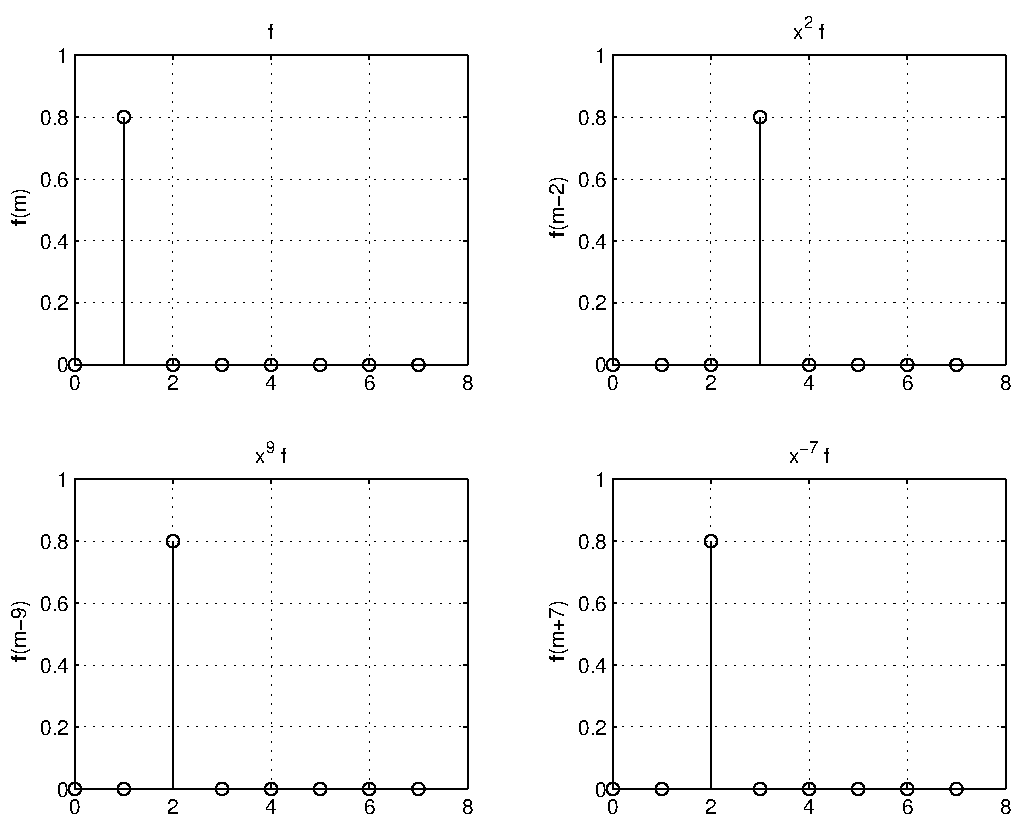
\includegraphics[width=\columnwidth]{t_cyclicshift}}}
  \caption{An impulse $f\in \CA$ and a few abelian group translates, $x^2f, x^9f,
      x^{-7}f$.}
  \label{fig:cyclicshift}
\end{figure}

%\begin{figure}
%%  \centerline{\epsfig{figure=figures/t_cyclicshift,width=70mm, height=50mm}}
%  \centering
%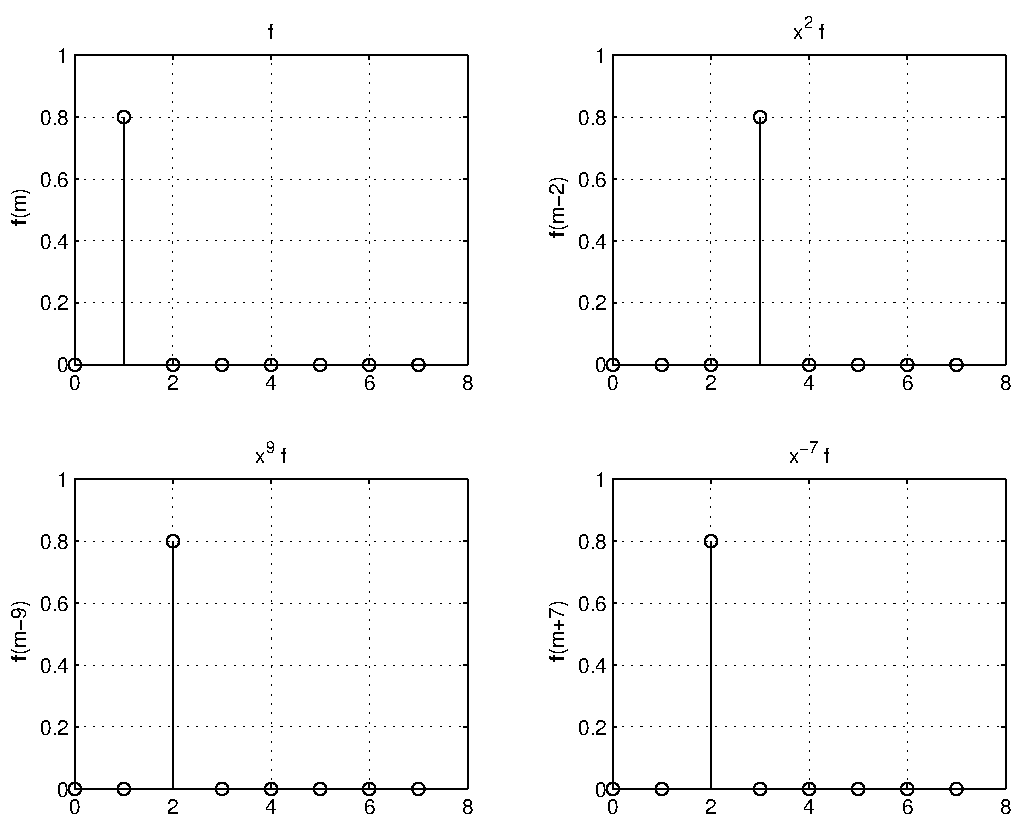
\includegraphics[width=80mm, height=70mm]{t_cyclicshift}
%  \caption{An impulse $f\in \CA$ and a few abelian group translates, $x^2f, x^9f,
%      x^{-7}f$.}
%  \label{fig:cyclicshift}
%\end{figure}

%------------------------------------------------------------------------
\subsection{Ideals: Translation-Invariant Subspaces}
%------------------------------------------------------------------------
A subspace $\vs{V}$ of the space $\CG$ is called a
\emph{left ideal} if 
\begin{equation}
u\vs{V} = \{uf : f \in \vs{V}\} \subset \vs{V}, \quad u \in G. 
\end{equation}
A left ideal of $\CG$ corresponds to a subspace of $\LG$
invariant under all left translations.  

If $\vs{V}$ is a left ideal, then, by linearity, 
$g\vs{V} \subset \vs{V}$ for all $g \in \CG$.
The set $\CG g$, defined by 
$\{fg : f \in \CG\}$, is a left ideal of $\CG$,
called \emph{the left ideal generated by} $g$ in $\CG$. 
%$\CG g = \CG$ if and only if $g$ is an invertible element in $\CG$. 
A left ideal $\vs{V}$ of $\CG$ is called \emph{irreducible}
if the only left ideals of $\CG$ contained in $\vs{V}$ are
$\{0\}$ and $\vs{V}$. The sum of two distinct, irreducible
left ideals is always a direct sum. 
% (\cite{An:2003}, p.~129).

For \emph{abelian} group $A$, the group algebra $\C A$ of
signals is decomposed into a direct sum of irreducible ideals.  
Since multiplication of $\C A$ by elements of $A$
corresponds to translation, ideals represent
translation-invariant subspaces.  Furthermore, in the 
abelian case, such translation-invariant subspaces are
one-dimensional.   

Similarly, for \emph{nonabelian} group $G$, the group algebra
$\CG$ is decomposed into a direct sum of left ideals. Here,
again, the ideals are translation-invariant 
subspaces.  However, some of these subspaces must now be
multi-dimensional, and herein lies the potential advantage
of using nonabelian groups for indexing the data. The left
translations are more general and represent a broader class of 
transformations. Therefore, projections of data into the
resulting left ideals can reveal more complicated partitions
and structures in the data as compared with the Fourier
components in the abelian group case. 
!

%-----------------------------------------------------------------------
\subsection{The Group Algebra $\CG$}
%-----------------------------------------------------------------------
\label{sec:groupalgebra}
The \emph{group algebra} $\CG$ is the space of all formal sums
\begin{equation}
f = \sum_{x\in G} f(x) x, \quad f(x) \in \C,
\end{equation}
with the following operations for $f, g \in \CG$:
\begin{equation}
f+g = \sum_{x\in G} (f(x) + g(x))x,
\end{equation}
\begin{equation}
\alpha f = \sum_{x\in G} (\alpha f(x)) x, 
           \quad \alpha \in \C,
\end{equation}
\begin{equation}
fg = \sum_{x\in G}\left(\sum_{y\in G} f(y)g(y^{-1}x)\right)x. 
\end{equation}

The mapping $\lt{L}(g)$ of $\CG$ defined by 
$\lt{L}(g)f = gf$
is a linear operator on the space $\CG$ called 
\emph{left multiplication by} $g$.  
Since $y\in G$ can be identified with the formal
sum $e_y \in \CG$ consisting of a single nonzero term,
\begin{equation}\label{eq:leftmult}
yf = \lt{L}(e_y)f = \sum_{x\in G}f(y^{-1}x) x.
\end{equation}
In relation to translation of $\LG$, (\ref{eq:leftmult}) is the
$\CG$ analog. Fig.~\ref{fig:cyclicshift} illustrates.

The mapping $\Theta: \LG \to \CG$ defined by
\begin{equation}\label{eq:iso}
\Theta(f) = \sum_{x\in G} f(x) x, \quad f\in \LG,
\end{equation}
is an algebra isomorphism of the convolution algebra $\LG$
onto the group algebra $\CG$.  
Thus we can identify
$\Theta(f)$ with $f$, using  context to decide whether
$f$ refers to the function in $\LG$ or the formal sum in
$\CG$.  

An important aspect of the foregoing isomorphism is the
correspondence between the translations of the spaces.
Translation of $\LG$ by $y\in G$ %$\T(y)$ 
corresponds to left multiplication of $\CG$ by $y\in G$.
%$\lt{L}(y)$ 
Convolution of $\LG$ by $f\in \LG$ corresponds to
left multiplication of $\CG$ by $f\in \CG$. 
%We state 
%these relations symbolically as follows:
%\begin{center}
%\begin{tabular}{ccc}
%  $\LG$ & $\simeq$ & $\CG$ \\
%  $\lt{T}(y)$ & $\leftrightarrow$ & $\lt{L}(y)$\\
%  $\lt{C}(f)$ & $\leftrightarrow$ & $\lt{L}(f)$
%\end{tabular}
%\end{center}

\begin{figure}
\centerline{\framebox{
	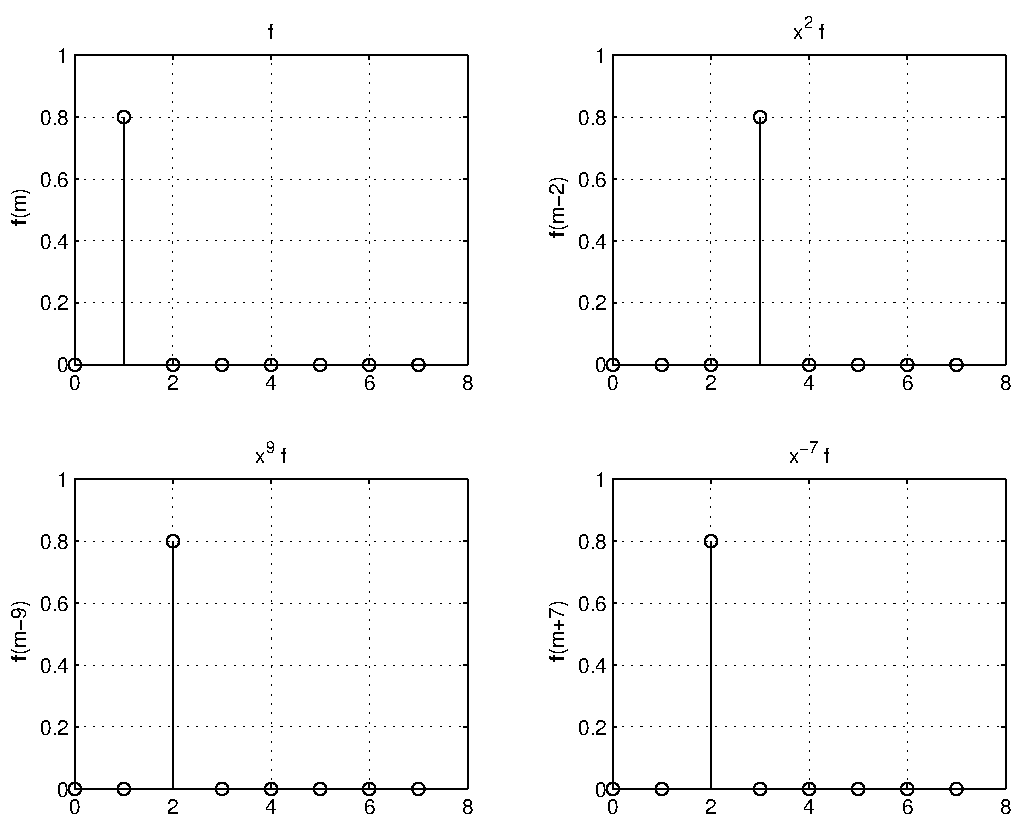
\includegraphics[width=\columnwidth]{t_cyclicshift}}}
  \caption{An impulse $f\in \CA$ and a few abelian group translates, $x^2f, x^9f,
      x^{-7}f$.}
  \label{fig:cyclicshift}
\end{figure}

%\begin{figure}
%%  \centerline{\epsfig{figure=figures/t_cyclicshift,width=70mm, height=50mm}}
%  \centering
%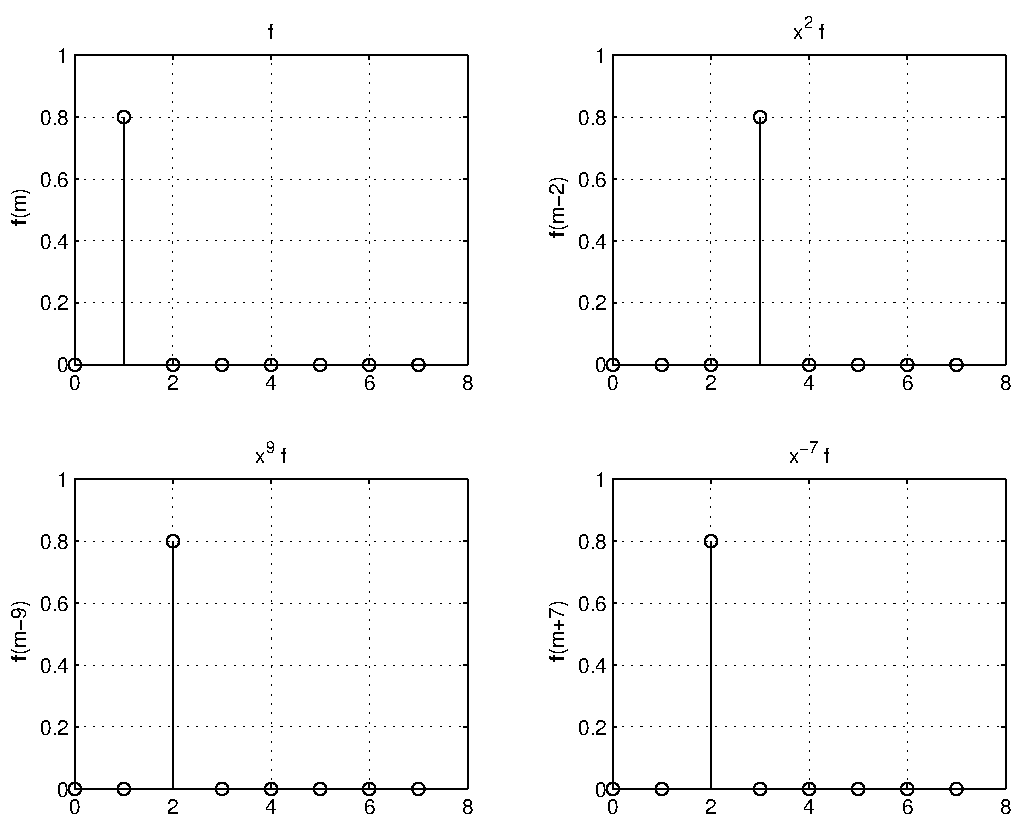
\includegraphics[width=80mm, height=70mm]{t_cyclicshift}
%  \caption{An impulse $f\in \CA$ and a few abelian group translates, $x^2f, x^9f,
%      x^{-7}f$.}
%  \label{fig:cyclicshift}
%\end{figure}

%------------------------------------------------------------------------
\subsection{Ideals: Translation-Invariant Subspaces}
%------------------------------------------------------------------------
A subspace $\vs{V}$ of the space $\CG$ is called a
\emph{left ideal} if 
\begin{equation}
u\vs{V} = \{uf : f \in \vs{V}\} \subset \vs{V}, \quad u \in G. 
\end{equation}
A left ideal of $\CG$ corresponds to a subspace of $\LG$
invariant under all left translations.  

If $\vs{V}$ is a left ideal, then, by linearity, 
$g\vs{V} \subset \vs{V}$ for all $g \in \CG$.
The set $\CG g$, defined by 
$\{fg : f \in \CG\}$, is a left ideal of $\CG$,
called \emph{the left ideal generated by} $g$ in $\CG$. 
%$\CG g = \CG$ if and only if $g$ is an invertible element in $\CG$. 
A left ideal $\vs{V}$ of $\CG$ is called \emph{irreducible}
if the only left ideals of $\CG$ contained in $\vs{V}$ are
$\{0\}$ and $\vs{V}$. The sum of two distinct, irreducible
left ideals is always a direct sum. 
% (\cite{An:2003}, p.~129).

For \emph{abelian} group $A$, the group algebra $\C A$ of
signals is decomposed into a direct sum of irreducible ideals.  
Since multiplication of $\C A$ by elements of $A$
corresponds to translation, ideals represent
translation-invariant subspaces.  Furthermore, in the 
abelian case, such translation-invariant subspaces are
one-dimensional.   

Similarly, for \emph{nonabelian} group $G$, the group algebra
$\CG$ is decomposed into a direct sum of left ideals. Here,
again, the ideals are translation-invariant 
subspaces.  However, some of these subspaces must now be
multi-dimensional, and herein lies the potential advantage
of using nonabelian groups for indexing the data. The left
translations are more general and represent a broader class of 
transformations. Therefore, projections of data into the
resulting left ideals can reveal more complicated partitions
and structures in the data as compared with the Fourier
components in the abelian group case. 


%--IDEALS---------------------------------------------------------------------------
\verb!%------------------------------------------------------------------------
\ismasubsec{Translation-Invariant Subspaces}
%------------------------------------------------------------------------
A subspace $\vs{V}$ of the space $\CG$ is called a
\emph{left ideal} if 
\begin{equation}
u\vs{V} = \{uf : f \in \vs{V}\} \subset \vs{V}, \quad u \in G. 
\end{equation}
A left ideal of $\CG$ corresponds to a subspace of $\LG$
invariant under all left translations.  If $\vs{V}$ is a
left ideal, then, by linearity, 
$g\vs{V} \subset \vs{V}$ for all $g \in \CG$.
The set $\CG g$, defined by 
$\{fg : f \in \CG\}$, is a left ideal of $\CG$,
called \emph{the left ideal generated by} $g$ in $\CG$. 
%$\CG g = \CG$ if and only if $g$ is an invertible element in $\CG$. 
A left ideal $\vs{V}$ of $\CG$ is called \emph{irreducible}
if the only left ideals of $\CG$ contained in $\vs{V}$ are
$\{0\}$ and $\vs{V}$. The sum of two distinct, irreducible
left ideals is always a direct sum. 
% (\cite{An:2003}, p.~129).

For \emph{abelian} group $A$, the group algebra $\C A$ of
signals is decomposed into a direct sum of irreducible ideals.  
Since multiplication of $\C A$ by elements of $G$
corresponds to translation, ideals represent
translation-invariant subspaces.  Furthermore, in the 
abelian case, such translation-invariant subspaces are
one-dimensional.   

Similarly, for \emph{nonabelian} group $G$, the group algebra
$\CG$ is decomposed into a direct sum of left ideals
and, again, the ideals are translation-invariant
subspaces.  However, some of them must now be multi-dimensional,
and herein lies the potential advantage of using nonabelian
groups for indexing the data. The left translations
are more general and represent a broader class of 
transformations. Therefore, projections of data into the
resulting left ideals can reveal more complicated partitions
and structures as compared with the Fourier components in
the abelian group case. 

!
%------------------------------------------------------------------------
\ismasubsec{Translation-Invariant Subspaces}
%------------------------------------------------------------------------
A subspace $\vs{V}$ of the space $\CG$ is called a
\emph{left ideal} if 
\begin{equation}
u\vs{V} = \{uf : f \in \vs{V}\} \subset \vs{V}, \quad u \in G. 
\end{equation}
A left ideal of $\CG$ corresponds to a subspace of $\LG$
invariant under all left translations.  If $\vs{V}$ is a
left ideal, then, by linearity, 
$g\vs{V} \subset \vs{V}$ for all $g \in \CG$.
The set $\CG g$, defined by 
$\{fg : f \in \CG\}$, is a left ideal of $\CG$,
called \emph{the left ideal generated by} $g$ in $\CG$. 
%$\CG g = \CG$ if and only if $g$ is an invertible element in $\CG$. 
A left ideal $\vs{V}$ of $\CG$ is called \emph{irreducible}
if the only left ideals of $\CG$ contained in $\vs{V}$ are
$\{0\}$ and $\vs{V}$. The sum of two distinct, irreducible
left ideals is always a direct sum. 
% (\cite{An:2003}, p.~129).

For \emph{abelian} group $A$, the group algebra $\C A$ of
signals is decomposed into a direct sum of irreducible ideals.  
Since multiplication of $\C A$ by elements of $G$
corresponds to translation, ideals represent
translation-invariant subspaces.  Furthermore, in the 
abelian case, such translation-invariant subspaces are
one-dimensional.   

Similarly, for \emph{nonabelian} group $G$, the group algebra
$\CG$ is decomposed into a direct sum of left ideals
and, again, the ideals are translation-invariant
subspaces.  However, some of them must now be multi-dimensional,
and herein lies the potential advantage of using nonabelian
groups for indexing the data. The left translations
are more general and represent a broader class of 
transformations. Therefore, projections of data into the
resulting left ideals can reveal more complicated partitions
and structures as compared with the Fourier components in
the abelian group case. 



%%=======================================================================
%\ismasec{Abelian Group DSP}
%%=======================================================================
%\verb!\input{DSP/abelianTranslation}!
%\input{DSP/abelianTranslation}
%\verb!\input{DSP/abelianDSP}!
%\input{DSP/abelianDSP}

%=======================================================================
\ismasec{Nonabelian Group DSP}
%=======================================================================
This section presents some basic theory of digital 
signal processing (DSP), but relies on a more general 
mathematical formalism than that employed by the 
standard textbooks on the subject.\footnote{A few notable
  exceptions are 
  \cite{{An:2003}, {Tolimieri:1998}}, {Chirikjian:2002}.}
%\cite{{An:2003},{Chirikjian:2001},{Tolimieri:1998},{Tolimieri:1997}}}.
%the book by Chirikjian and Kyatkin~  %and the books by Tolimieri and An

%--NONABELIAN---------------------------------------------------------------------------
%\verb!\input{DSP/nonabelianDSP}!
%\input{DSP/nonabelianDSP}
%\verb!\input{DSP/nonabelianDSP-long}!
%\input{DSP/nonabelianDSP-long}
%\verb!\input{DSP/hafg-nonabelian}!
%\input{DSP/hafg-nonabelianDSP}

\verb!
%=======================================================================
\section{Nonabelian Group DSP}
%=======================================================================
This section presents some basic principles of
DSP, but relies on a more general mathematical formalism
than that commonly found in textbooks on the subject.\footnote{A few notable
  exceptions are~\cite{An:2003, Tolimieri:2003, Tolimieri:1998, Chirikjian:2002}.}
%\cite{{An:2003},{Chirikjian:2001},{Tolimieri:1998},{Tolimieri:1997}}}.
%the book by Chirikjian and Kyatkin~  %and the books by Tolimieri and An

%------------------------------------------------------------------------
\subsection{The Group of Characters: Main Theorems}
%------------------------------------------------------------------------
A \emph{character} of $G$ is a group homomorphism of $G$
into $\C^{\times}$, where $\C^{\times} = \C \setminus \{0\}$.
In other words, the mapping $\varrho: G \to \C^{\times}$ is 
a character of $G$ if it satisfies 
$\varrho(xy) = \varrho(x)\varrho(y), \, x, y \in G$.
%There is always at least one character, the 
%\emph{trivial character}, which is 1 for all $y\in G$. 
Let $G^*$ denote the set of all characters of $G$.

By the identification~(\ref{eq:iso}) between $\LG$ and
$\CG$, a character $\varrho \in G^*$ can be viewed as
a formal sum,
\begin{equation}
\varrho = \sum_{x\in G}\varrho(x)x.
\end{equation}
Therefore, $G^* \subset \CG$. 
Expressing the characters as formal sums 
leads to simple proofs of important DSP results.
%%%
%%% T-1
%%%
\begin{theorem}\label{thm:char-action}     
If $\varrho$ is a character of $G$, then
\begin{equation}
y\varrho = \varrho y = \varrho(y^{-1})\varrho, \quad y\in G.
\end{equation}
\end{theorem}
\begin{proof}
%%%
%%% P-1
%%%
By a change of variables,
\[
\varrho y = \sum_{x\in G}\varrho(x)xy = \sum_{x\in G}\varrho(xy^{-1})x, \quad y\in G.
\]
By homomorphism property, $\varrho(xy^{-1}) =
\varrho(x)\varrho(y^{-1})$.  Therefore, 
\[
\varrho y %=\sum_{x\in G}\varrho(xy^{-1})x 
= \sum_{x\in G}\varrho(x)\varrho(y^{-1})x
= \varrho(y^{-1})\varrho, \quad y\in G.
\]
A similar change of variables argument shows
\[
y\varrho %= \sum_{x\in G}\varrho(x)yx
= \sum_{x\in G}\varrho(y^{-1}x)x
= \varrho(y^{-1})\varrho, \quad y\in G.
\]
%As above, write $\varrho$ as a formal sum and change
%variables.
%% \qed
\end{proof}
%\begin{proof}By a change of variables,\begin{equation}
%\varrho y = \sum_{x\in G}\varrho(x)xy = \sum_{x\in G}\varrho(xy^{-1})x, \quad y\in G.
%\end{equation}By homomorphism property, $\varrho(xy^{-1}) =
%\varrho(x)\varrho(y^{-1})$.  Therefore, $\varrho y = \varrho(y^{-1})\varrho$, for all $\quad y\in G$.
%The same change of variables argument works for $y\varrho$.\qed\end{proof}
%%%
%%% T-2
%%%
\begin{theorem}\label{thm:eigenvector}             
%If $\varrho\in G^*$ is a nontrivial character of $G$, then
For $\varrho\in G^*$,
\begin{equation}
\frac{1}{|G|} \sum_{x\in G} \varrho(x) = 
\begin{cases}  1, & \varrho(x)=1, \forall x\in G,\\
0, & \text{otherwise.}
\end{cases}
\end{equation}
\end{theorem}
where $|G|$ is the order of $G$.
%%%
%%% P-2
%%%
\begin{proof}
%%Let $y\in G$ be such that $\varrho(y) \neq 0$, and $\varrho(y) \neq 1$.  (If no
%%such $y$ exists, the result is obvious.)
By a change of variables,
\begin{equation}
\varrho(y) \sum_{x\in G} \varrho(x) = \sum_{x\in G}
\varrho(yx) = \sum_{x\in G} \varrho(x), \quad y\in G.
\end{equation}
Thus, either $\varrho(x)=1, \forall x\in G$, 
or $\sum \varrho(x)=0$.
\end{proof}
%\qed 

Theorem~\ref{thm:char-action} shows that every character is
an eigenvector of left-multiplication by elements of the
group $G$, so we call them $\lt{L}(G)$-eigenvectors.
Therefore, by linearity, the characters are eigenvectors
of left-multiplication by $f\in \CG$ (convolution by
$f\in \LG$).  This is re-stated more formally as the following
formula for the $G$-\emph{spectral components} of $f$:
\begin{corollary}\label{cor:FT}
If $\varrho\in G^*$ and $f\in \CG$, then
\begin{equation}\label{eq:FT}
f\varrho = \varrho f = \hat{f}(\varrho)\varrho,
\end{equation}
where $\hat{f}(\varrho) = \sum_{y\in G} f(y) \varrho(y^{-1})$.
%\end{cor}
\end{corollary}
\begin{proof}
By Theorem~\ref{thm:char-action},
\begin{equation}
f\varrho = \sum_{y\in G} f(y) y\varrho =  \sum_{y\in G} f(y)\varrho(y^{-1}) \varrho
\end{equation}
Similarly for $\varrho f$, mutatis mutandis.
%\qed
\end{proof}

The functions which make up the standard Fourier basis
% -- the exponential functions -- 
are eigenvectors of standard convolution.  
As seen in the foregoing proofs, % of~\ref{thm:eigenvector}, 
this is merely a consequence of the fact that the
exponential functions are %satisfy properties which allow usto call them 
characters.  \emph{The notion of a character basis
generalizes the Fourier basis to include bases which
can diagonalize any linear combination of 
left group multiplications.}
%%% LEFT OFF with notes on p. 132 %%%
\begin{corollary}\label{cor:idemp}
If $\lambda, \tau \in G^*$, then
\begin{equation}
\lambda \tau = 
\begin{cases}  |G|\lambda, & \tau=\lambda,\\
0, & \tau\neq\lambda.
\end{cases}
\end{equation}
\end{corollary}
\begin{proof}
Suppose $\tau = \lambda$; then,
%\begin{eqnarray*}
\[\lambda \tau %= \lambda\lambda &=& \sum_{x\in G} \tau(x)x\tau\\
= \sum_{x\in G} \lambda(x)\lambda(x^{-1})\lambda
= \sum_{x\in G} \lambda(1)\lambda = |G|\lambda
\]%\end{eqnarray*}
Suppose $\tau \neq \lambda$. By definition,
\begin{equation}
\hat{\lambda}(\tau) = \sum_{x\in G}\lambda(x)\tau(x^{-1}) =
\sum_{y\in G}\lambda(y^{-1})\tau(y) = \hat{\tau}(\lambda)
\end{equation}
By~(\ref{eq:FT}), 
$\hat{\lambda}(\tau)\tau = \lambda\tau = \tau\lambda =\hat{\tau}(\lambda)\lambda $.  
Since $\hat{\lambda}(\tau) = \hat{\tau}(\lambda)$ and $\tau
\neq \lambda$, it must be the case that
$\hat{\tau} = 0$ and $\lambda\tau = 0$.
%\qed
\end{proof}
Corollary~\ref{cor:idemp} can be expressed in the language
of \emph{idempotent theory}.  A nonzero element $e \in \CG$
is called an \emph{idempotent} if $e^2 = e$. Two idempotents
$e_1$ and $e_2$ are called orthogonal if
$e_1e_2 = e_2e_1 = 0$.
Corollary~\ref{cor:idemp} says that 
\[
\left\{\frac{1}{|G|}\rho : \rho \in G^* \right\}
\]
is a set of pairwise orthogonal idempotents.

!

%=======================================================================
\section{Nonabelian Group DSP}
%=======================================================================
This section presents some basic principles of
DSP, but relies on a more general mathematical formalism
than that commonly found in textbooks on the subject.\footnote{A few notable
  exceptions are~\cite{An:2003, Tolimieri:2003, Tolimieri:1998, Chirikjian:2002}.}
%\cite{{An:2003},{Chirikjian:2001},{Tolimieri:1998},{Tolimieri:1997}}}.
%the book by Chirikjian and Kyatkin~  %and the books by Tolimieri and An

%------------------------------------------------------------------------
\subsection{The Group of Characters: Main Theorems}
%------------------------------------------------------------------------
A \emph{character} of $G$ is a group homomorphism of $G$
into $\C^{\times}$, where $\C^{\times} = \C \setminus \{0\}$.
In other words, the mapping $\varrho: G \to \C^{\times}$ is 
a character of $G$ if it satisfies 
$\varrho(xy) = \varrho(x)\varrho(y), \, x, y \in G$.
%There is always at least one character, the 
%\emph{trivial character}, which is 1 for all $y\in G$. 
Let $G^*$ denote the set of all characters of $G$.

By the identification~(\ref{eq:iso}) between $\LG$ and
$\CG$, a character $\varrho \in G^*$ can be viewed as
a formal sum,
\begin{equation}
\varrho = \sum_{x\in G}\varrho(x)x.
\end{equation}
Therefore, $G^* \subset \CG$. 
Expressing the characters as formal sums 
leads to simple proofs of important DSP results.
%%%
%%% T-1
%%%
\begin{theorem}\label{thm:char-action}     
If $\varrho$ is a character of $G$, then
\begin{equation}
y\varrho = \varrho y = \varrho(y^{-1})\varrho, \quad y\in G.
\end{equation}
\end{theorem}
\begin{proof}
%%%
%%% P-1
%%%
By a change of variables,
\[
\varrho y = \sum_{x\in G}\varrho(x)xy = \sum_{x\in G}\varrho(xy^{-1})x, \quad y\in G.
\]
By homomorphism property, $\varrho(xy^{-1}) =
\varrho(x)\varrho(y^{-1})$.  Therefore, 
\[
\varrho y %=\sum_{x\in G}\varrho(xy^{-1})x 
= \sum_{x\in G}\varrho(x)\varrho(y^{-1})x
= \varrho(y^{-1})\varrho, \quad y\in G.
\]
A similar change of variables argument shows
\[
y\varrho %= \sum_{x\in G}\varrho(x)yx
= \sum_{x\in G}\varrho(y^{-1}x)x
= \varrho(y^{-1})\varrho, \quad y\in G.
\]
%As above, write $\varrho$ as a formal sum and change
%variables.
%% \qed
\end{proof}
%\begin{proof}By a change of variables,\begin{equation}
%\varrho y = \sum_{x\in G}\varrho(x)xy = \sum_{x\in G}\varrho(xy^{-1})x, \quad y\in G.
%\end{equation}By homomorphism property, $\varrho(xy^{-1}) =
%\varrho(x)\varrho(y^{-1})$.  Therefore, $\varrho y = \varrho(y^{-1})\varrho$, for all $\quad y\in G$.
%The same change of variables argument works for $y\varrho$.\qed\end{proof}
%%%
%%% T-2
%%%
\begin{theorem}\label{thm:eigenvector}             
%If $\varrho\in G^*$ is a nontrivial character of $G$, then
For $\varrho\in G^*$,
\begin{equation}
\frac{1}{|G|} \sum_{x\in G} \varrho(x) = 
\begin{cases}  1, & \varrho(x)=1, \forall x\in G,\\
0, & \text{otherwise.}
\end{cases}
\end{equation}
\end{theorem}
where $|G|$ is the order of $G$.
%%%
%%% P-2
%%%
\begin{proof}
%%Let $y\in G$ be such that $\varrho(y) \neq 0$, and $\varrho(y) \neq 1$.  (If no
%%such $y$ exists, the result is obvious.)
By a change of variables,
\begin{equation}
\varrho(y) \sum_{x\in G} \varrho(x) = \sum_{x\in G}
\varrho(yx) = \sum_{x\in G} \varrho(x), \quad y\in G.
\end{equation}
Thus, either $\varrho(x)=1, \forall x\in G$, 
or $\sum \varrho(x)=0$.
\end{proof}
%\qed 

Theorem~\ref{thm:char-action} shows that every character is
an eigenvector of left-multiplication by elements of the
group $G$, so we call them $\lt{L}(G)$-eigenvectors.
Therefore, by linearity, the characters are eigenvectors
of left-multiplication by $f\in \CG$ (convolution by
$f\in \LG$).  This is re-stated more formally as the following
formula for the $G$-\emph{spectral components} of $f$:
\begin{corollary}\label{cor:FT}
If $\varrho\in G^*$ and $f\in \CG$, then
\begin{equation}\label{eq:FT}
f\varrho = \varrho f = \hat{f}(\varrho)\varrho,
\end{equation}
where $\hat{f}(\varrho) = \sum_{y\in G} f(y) \varrho(y^{-1})$.
%\end{cor}
\end{corollary}
\begin{proof}
By Theorem~\ref{thm:char-action},
\begin{equation}
f\varrho = \sum_{y\in G} f(y) y\varrho =  \sum_{y\in G} f(y)\varrho(y^{-1}) \varrho
\end{equation}
Similarly for $\varrho f$, mutatis mutandis.
%\qed
\end{proof}

The functions which make up the standard Fourier basis
% -- the exponential functions -- 
are eigenvectors of standard convolution.  
As seen in the foregoing proofs, % of~\ref{thm:eigenvector}, 
this is merely a consequence of the fact that the
exponential functions are %satisfy properties which allow usto call them 
characters.  \emph{The notion of a character basis
generalizes the Fourier basis to include bases which
can diagonalize any linear combination of 
left group multiplications.}
%%% LEFT OFF with notes on p. 132 %%%
\begin{corollary}\label{cor:idemp}
If $\lambda, \tau \in G^*$, then
\begin{equation}
\lambda \tau = 
\begin{cases}  |G|\lambda, & \tau=\lambda,\\
0, & \tau\neq\lambda.
\end{cases}
\end{equation}
\end{corollary}
\begin{proof}
Suppose $\tau = \lambda$; then,
%\begin{eqnarray*}
\[\lambda \tau %= \lambda\lambda &=& \sum_{x\in G} \tau(x)x\tau\\
= \sum_{x\in G} \lambda(x)\lambda(x^{-1})\lambda
= \sum_{x\in G} \lambda(1)\lambda = |G|\lambda
\]%\end{eqnarray*}
Suppose $\tau \neq \lambda$. By definition,
\begin{equation}
\hat{\lambda}(\tau) = \sum_{x\in G}\lambda(x)\tau(x^{-1}) =
\sum_{y\in G}\lambda(y^{-1})\tau(y) = \hat{\tau}(\lambda)
\end{equation}
By~(\ref{eq:FT}), 
$\hat{\lambda}(\tau)\tau = \lambda\tau = \tau\lambda =\hat{\tau}(\lambda)\lambda $.  
Since $\hat{\lambda}(\tau) = \hat{\tau}(\lambda)$ and $\tau
\neq \lambda$, it must be the case that
$\hat{\tau} = 0$ and $\lambda\tau = 0$.
%\qed
\end{proof}
Corollary~\ref{cor:idemp} can be expressed in the language
of \emph{idempotent theory}.  A nonzero element $e \in \CG$
is called an \emph{idempotent} if $e^2 = e$. Two idempotents
$e_1$ and $e_2$ are called orthogonal if
$e_1e_2 = e_2e_1 = 0$.
Corollary~\ref{cor:idemp} says that 
\[
\left\{\frac{1}{|G|}\rho : \rho \in G^* \right\}
\]
is a set of pairwise orthogonal idempotents.



%--THEOREMS----------------------------------------------------------------------
%\verb!\input{DSP/ngdsp-theorems}!
%\input{DSP/ngdsp-theorems}

%--SDP---------------------------------------------------------------------------
\verb!% This is the master sdp.tex file -- the most
% up-to-date -- the one on which all others are based.

% UHEE616-sdp.tex integrated on 2005.03.16

%----------------------------------------------------------------------
\subsection{Semidirect Product Groups}
%----------------------------------------------------------------------
To determine whether a particular group is useful for a DSP
application, we must specify exactly how this group
represents the data.
The group representation may reduce computational
complexity, or it may simply make it easier to state,
understand, or model a given signal processing task.

This section describes %procedures for specifying and studying 
a simple class of nonabelian groups that have
proven useful in applications -- 
\emph{abelian by abelian semidirect products}. 
%These are
%perhaps the simplest extension of abelian groups
%% case, these are
%%groups of the form $G = A \sdp B$, where $A$ and $B$
%%are abelian groups. Not surprisingly, 
%and DSP over such groups closely resembles that over abelian
%groups.  However, the resulting processing tools can have
%vastly different characteristics. 

%%% LEFT OFF HERE --> resume from top of page 109
%%% LEFT OFF with notes on p. 132 %%%

%-----------------------------------------------------------------------
%\ismasubsec{Action Group}
%-----------------------------------------------------------------------
Let $G$ be a finite group of order $N$, $K$ a subgroup of $G$,
and $H$ a normal subgroup of $G$. If $G = HK$ and $H \cap
K = \{1\}$, then we say that $G$ is the 
%\emph{internal semidirect product}
\emph{semidirect product} $G = H \sdp K$. 
It can be shown that $G = H \sdp K$ if and only if every $x \in
G$ has a unique representation of the form $x = yz, \; y\in H,
z\in K$.

Denote by $Aut(H)$ the set of all \emph{automorphisms} of
$H$. The mapping $\Psi:K\rightarrow Aut(H)$ defined by  
\begin{equation}\label{eq:homo}
\Psi_z(x) = zxz^{-1}, \quad z\in K, x\in H
\end{equation}
is a group homomorphism. 
Define the binary composition in $G$
%relative to the representation $G= H\sdp K$
in terms of $\Psi$ as follows:
\begin{equation}\label{eq:PsiProd}
x_1x_2 = (y_1z_1)(y_2z_2)= y_1\Psi_{z_1}(y_2)z_1z_2,
\end{equation}
\[
y_1, y_2 \in H,\; z_1, z_2 \in K. 
\]

If $K$ is a normal subgroup of $G$,
then $y^{-1}Ky = K$ for all $y\in G$, 
%(by definition of \emph{normal subgroup}) in which case, %$[H, K] = \{1\}$, 
and $G$ is simply the cartesian product $H\times K$ 
with component-wise multiplication. 
What is new in the semidirect product is
the possibility that $K$ acts nontrivially on $H$. 
For this reason, $K$ is sometimes called the ``action group.''

%-----------------------------------------------------------------------
\subsubsection{Simplest Nonabelian Example}
%-----------------------------------------------------------------------
If the mapping $\Psi$ given in~(\ref{eq:homo}) is defined over
$K=U(N)$, then $\Psi$ is a group isomorphism.
Under this identification, we can form the semidirect
product $G = H\sdp K$, with $H = C_N(x)$ and $K$ a
subgroup of $U(N)$.  Throughout this section, $G$ will
denote such a semidirect product group.

The elements $u\in K$ are integers. However, following~\cite{An:2003} we
denote by $k_u$ the element $u\in K$, as this avoids confusion that can arise 
on occasion. This notation is especially useful when $K$ 
is a cyclic group with generator $u$.  If  we denote elements of $K$ by $k_u^j$, instead of 
by $u^j$, it is easier to distinguish them from elements of the abelian group $C_N(x)$.

Suppose the action group $K$ is a cyclic group of order $J = |K|$ with generator
$u$. We identify each element of $K$ with an index, and denote 
the set of elements by $K = \{k_u^j: 0\leq j < J\}$.
Thus, to each $k_v \in K$, there corresponds a $j\in \Z$ 
such that $k_u^j=k_v$.
We use $x^n k_v$ and $x^n k_u^j$ to denote  
typical points of $G=C_N(x)\sdp K$.

Given two points in $G$, say $z = x^m k_u$
and $y=x^n k_v$, define multiplication %on $G$ 
according
to~(\ref{eq:PsiProd}) as follows:
\begin{equation}\label{eq:prod}
  zy = (x^m k_u)(x^n k_v) = x^{m+u n} k_u k_v,
\end{equation}
where %In~(\ref{eq:prod}), 
$m+ u n$ is taken modulo $N$.
Since $k_v=k_u^j$ for some $j\in \Z$, then 
$k_u k_v = k_u^{1+j}$, and $zy = x^{m+u n} k_u^{j+1}$.

Let $z = x^m k_v$ and suppose $k_w$ is the inverse 
of $k_v$ in $K$.  Then the inverse of $z$ must be
$z^{-1}=x^{N-wm} k_w$, since this satisfies
%\begin{equation}\label{eq:inv}z^{-1}=x^{N-wm} k_w.\end{equation}
$\inverse{z}z \equiv 1$.

Suppose $K \subset U(N)$ has order $|K|=J$, 
and consider the semidirect product group
with elements
\begin{equation}
  G   = \{x^n k_u^j : 0 \leq n < N, 0 \leq j < J\}.\label{eq:sdp}
\end{equation}
%\ismasubsec{Translations on Semidirect Product Groups}
For $f\in \CG$, %the formal sum can be expressed in the following ways:
\begin{equation}
  f = \sum_{y\in G} f(y)y= \sum_{n,j} f(x^n k_u^j)x^n k_u^j,
\end{equation}
%where $0\leq n <N$ and $0\leq j < J$.

As above, translations of $\CG$ are defined as
left multiplication by elements of $G$.  
For semidirect product~(\ref{eq:sdp}) 
there is a simple dichotomy of translation types that arise
from left-multiplication by elements of $G$.  %Translations of the
First, the familiar ``abelian translates'' 
are obtained upon left-multiplication by powers of $x$
(Fig.~\ref{fig:cyclicshift}).  
By change of variables, 
\begin{equation}\label{eq:1}
x^mf = \sum_{n,j} f(x^{n-m} k_u^j)x^n k_u^j,
\end{equation}
which is simply a right shift of $f$ by $m$ units.
Similarly, left-multiplication by powers of
$x^{-1}$ effects left shift of $f$. 
(Recall, $x^{-1} \equiv x^{N-1}$
and $x^{-m} \equiv x^{N-m}$.)  

Of the second type are the ``nonabelian translates,'' 
obtained upon left-multiplication by $k_v \in K$.
\begin{equation}
  k_vf %&=& \sum_{n,j} f(x^n k_u^j)k_v x^n k_u^j\nonumber\\
  = \sum_{n,j} f(k_v^{-1}x^n k_u^j)x^n k_u^j.
\end{equation}
Suppose $k_w = k_u^\ell$ is the inverse of $k_v$ in $K$.  Then,
\begin{equation}
  k_vf %  &=& \sum_{n,j} f(k_w x^{n}k_u^j)x^n k_u^j\nonumber\\
  = \sum_{n,j} f(x^{wn}k_u^{\ell + j})x^n k_u^j\label{eq:nonabtrans}
\end{equation}
%As usual, summation is over $0\leq n <N$ and $0\leq j < J$.
From equation~(\ref{eq:nonabtrans}) it is clear that $k_vf$ 
results in a more complex transformation than that of 
$x^m f$ as given by~(\ref{eq:1}).

%\newcommand{\zmv}{\ensuremath{x^m k_v}}
%\newcommand{\zmvInv}{\ensuremath{x^{N-wm} k_w}}

For the general element $z = \zmv \in G$ with 
inverse $z^{-1}=\zmvInv$ %(equation~(\ref{eq:inv})), 
we derive rules for generalized translations.
% with respect to $z$ and $z^{-1}$.
\begin{equation*}
  zf = \sum_{y\in G} f(z^{-1}y)y= \sum_{n,j} f(x^{N-w(m-n)} k_w k_u^j)x^n k_u^j
%  &=& \sum_{y\in G} f(y)zy = \sum_{y\in G} f(z^{-1}y)y\nonumber \\  
%  &=& \sum_{n,j} f(\zmvInv \, x^n k_u^j) x^n k_u^j\nonumber\\
%  &=& \sum_{n,j} f(x^{N-w(m-n)} k_w k_u^j)x^n k_u^j
\end{equation*}
\begin{equation*}
  z^{-1}f = \sum_{y\in G} f(zy)y= \sum_{n,j} f(x^{m+vn} k_vk_u^j)x^n k_u^j
%  &=& \sum_{y\in G} f(y)z^{-1}y = \sum_{y\in G} f(zy)y\nonumber \\  
%  &=& \sum_{n,j} f(\zmv x^n k_u^j)x^n k_u^j\nonumber\\
%  &=& \sum_{n,j} f(x^{m+vn} k_vk_u^j)x^n k_u^j
\end{equation*}

!
% This is the master sdp.tex file -- the most
% up-to-date -- the one on which all others are based.

% UHEE616-sdp.tex integrated on 2005.03.16

%----------------------------------------------------------------------
\subsection{Semidirect Product Groups}
%----------------------------------------------------------------------
To determine whether a particular group is useful for a DSP
application, we must specify exactly how this group
represents the data.
The group representation may reduce computational
complexity, or it may simply make it easier to state,
understand, or model a given signal processing task.

This section describes %procedures for specifying and studying 
a simple class of nonabelian groups that have
proven useful in applications -- 
\emph{abelian by abelian semidirect products}. 
%These are
%perhaps the simplest extension of abelian groups
%% case, these are
%%groups of the form $G = A \sdp B$, where $A$ and $B$
%%are abelian groups. Not surprisingly, 
%and DSP over such groups closely resembles that over abelian
%groups.  However, the resulting processing tools can have
%vastly different characteristics. 

%%% LEFT OFF HERE --> resume from top of page 109
%%% LEFT OFF with notes on p. 132 %%%

%-----------------------------------------------------------------------
%\ismasubsec{Action Group}
%-----------------------------------------------------------------------
Let $G$ be a finite group of order $N$, $K$ a subgroup of $G$,
and $H$ a normal subgroup of $G$. If $G = HK$ and $H \cap
K = \{1\}$, then we say that $G$ is the 
%\emph{internal semidirect product}
\emph{semidirect product} $G = H \sdp K$. 
It can be shown that $G = H \sdp K$ if and only if every $x \in
G$ has a unique representation of the form $x = yz, \; y\in H,
z\in K$.

Denote by $Aut(H)$ the set of all \emph{automorphisms} of
$H$. The mapping $\Psi:K\rightarrow Aut(H)$ defined by  
\begin{equation}\label{eq:homo}
\Psi_z(x) = zxz^{-1}, \quad z\in K, x\in H
\end{equation}
is a group homomorphism. 
Define the binary composition in $G$
%relative to the representation $G= H\sdp K$
in terms of $\Psi$ as follows:
\begin{equation}\label{eq:PsiProd}
x_1x_2 = (y_1z_1)(y_2z_2)= y_1\Psi_{z_1}(y_2)z_1z_2,
\end{equation}
\[
y_1, y_2 \in H,\; z_1, z_2 \in K. 
\]

If $K$ is a normal subgroup of $G$,
then $y^{-1}Ky = K$ for all $y\in G$, 
%(by definition of \emph{normal subgroup}) in which case, %$[H, K] = \{1\}$, 
and $G$ is simply the cartesian product $H\times K$ 
with component-wise multiplication. 
What is new in the semidirect product is
the possibility that $K$ acts nontrivially on $H$. 
For this reason, $K$ is sometimes called the ``action group.''

%-----------------------------------------------------------------------
\subsubsection{Simplest Nonabelian Example}
%-----------------------------------------------------------------------
If the mapping $\Psi$ given in~(\ref{eq:homo}) is defined over
$K=U(N)$, then $\Psi$ is a group isomorphism.
Under this identification, we can form the semidirect
product $G = H\sdp K$, with $H = C_N(x)$ and $K$ a
subgroup of $U(N)$.  Throughout this section, $G$ will
denote such a semidirect product group.

The elements $u\in K$ are integers. However, following~\cite{An:2003} we
denote by $k_u$ the element $u\in K$, as this avoids confusion that can arise 
on occasion. This notation is especially useful when $K$ 
is a cyclic group with generator $u$.  If  we denote elements of $K$ by $k_u^j$, instead of 
by $u^j$, it is easier to distinguish them from elements of the abelian group $C_N(x)$.

Suppose the action group $K$ is a cyclic group of order $J = |K|$ with generator
$u$. We identify each element of $K$ with an index, and denote 
the set of elements by $K = \{k_u^j: 0\leq j < J\}$.
Thus, to each $k_v \in K$, there corresponds a $j\in \Z$ 
such that $k_u^j=k_v$.
We use $x^n k_v$ and $x^n k_u^j$ to denote  
typical points of $G=C_N(x)\sdp K$.

Given two points in $G$, say $z = x^m k_u$
and $y=x^n k_v$, define multiplication %on $G$ 
according
to~(\ref{eq:PsiProd}) as follows:
\begin{equation}\label{eq:prod}
  zy = (x^m k_u)(x^n k_v) = x^{m+u n} k_u k_v,
\end{equation}
where %In~(\ref{eq:prod}), 
$m+ u n$ is taken modulo $N$.
Since $k_v=k_u^j$ for some $j\in \Z$, then 
$k_u k_v = k_u^{1+j}$, and $zy = x^{m+u n} k_u^{j+1}$.

Let $z = x^m k_v$ and suppose $k_w$ is the inverse 
of $k_v$ in $K$.  Then the inverse of $z$ must be
$z^{-1}=x^{N-wm} k_w$, since this satisfies
%\begin{equation}\label{eq:inv}z^{-1}=x^{N-wm} k_w.\end{equation}
$\inverse{z}z \equiv 1$.

Suppose $K \subset U(N)$ has order $|K|=J$, 
and consider the semidirect product group
with elements
\begin{equation}
  G   = \{x^n k_u^j : 0 \leq n < N, 0 \leq j < J\}.\label{eq:sdp}
\end{equation}
%\ismasubsec{Translations on Semidirect Product Groups}
For $f\in \CG$, %the formal sum can be expressed in the following ways:
\begin{equation}
  f = \sum_{y\in G} f(y)y= \sum_{n,j} f(x^n k_u^j)x^n k_u^j,
\end{equation}
%where $0\leq n <N$ and $0\leq j < J$.

As above, translations of $\CG$ are defined as
left multiplication by elements of $G$.  
For semidirect product~(\ref{eq:sdp}) 
there is a simple dichotomy of translation types that arise
from left-multiplication by elements of $G$.  %Translations of the
First, the familiar ``abelian translates'' 
are obtained upon left-multiplication by powers of $x$
(Fig.~\ref{fig:cyclicshift}).  
By change of variables, 
\begin{equation}\label{eq:1}
x^mf = \sum_{n,j} f(x^{n-m} k_u^j)x^n k_u^j,
\end{equation}
which is simply a right shift of $f$ by $m$ units.
Similarly, left-multiplication by powers of
$x^{-1}$ effects left shift of $f$. 
(Recall, $x^{-1} \equiv x^{N-1}$
and $x^{-m} \equiv x^{N-m}$.)  

Of the second type are the ``nonabelian translates,'' 
obtained upon left-multiplication by $k_v \in K$.
\begin{equation}
  k_vf %&=& \sum_{n,j} f(x^n k_u^j)k_v x^n k_u^j\nonumber\\
  = \sum_{n,j} f(k_v^{-1}x^n k_u^j)x^n k_u^j.
\end{equation}
Suppose $k_w = k_u^\ell$ is the inverse of $k_v$ in $K$.  Then,
\begin{equation}
  k_vf %  &=& \sum_{n,j} f(k_w x^{n}k_u^j)x^n k_u^j\nonumber\\
  = \sum_{n,j} f(x^{wn}k_u^{\ell + j})x^n k_u^j\label{eq:nonabtrans}
\end{equation}
%As usual, summation is over $0\leq n <N$ and $0\leq j < J$.
From equation~(\ref{eq:nonabtrans}) it is clear that $k_vf$ 
results in a more complex transformation than that of 
$x^m f$ as given by~(\ref{eq:1}).

%\newcommand{\zmv}{\ensuremath{x^m k_v}}
%\newcommand{\zmvInv}{\ensuremath{x^{N-wm} k_w}}

For the general element $z = \zmv \in G$ with 
inverse $z^{-1}=\zmvInv$ %(equation~(\ref{eq:inv})), 
we derive rules for generalized translations.
% with respect to $z$ and $z^{-1}$.
\begin{equation*}
  zf = \sum_{y\in G} f(z^{-1}y)y= \sum_{n,j} f(x^{N-w(m-n)} k_w k_u^j)x^n k_u^j
%  &=& \sum_{y\in G} f(y)zy = \sum_{y\in G} f(z^{-1}y)y\nonumber \\  
%  &=& \sum_{n,j} f(\zmvInv \, x^n k_u^j) x^n k_u^j\nonumber\\
%  &=& \sum_{n,j} f(x^{N-w(m-n)} k_w k_u^j)x^n k_u^j
\end{equation*}
\begin{equation*}
  z^{-1}f = \sum_{y\in G} f(zy)y= \sum_{n,j} f(x^{m+vn} k_vk_u^j)x^n k_u^j
%  &=& \sum_{y\in G} f(y)z^{-1}y = \sum_{y\in G} f(zy)y\nonumber \\  
%  &=& \sum_{n,j} f(\zmv x^n k_u^j)x^n k_u^j\nonumber\\
%  &=& \sum_{n,j} f(x^{m+vn} k_vk_u^j)x^n k_u^j
\end{equation*}



%=======================================================================
\ismasec{Examples}
%=======================================================================
As seen above, when varying group structures are placed on indexing sets,
and products in the resulting group algebra are computed, 
interesting signal transforms obtain.  In this section,
we elucidate the nature of these operations by
examining some simple concrete examples in detail.

%--EXAMPLES-----------------------------------------------------------------
\verb!% This is the master examples.tex file -- the most
% up-to-date -- the one on which all others are based.
%
% ICMC2005-examples.tex was integrated on 2005.03.16.
% UHEE616-examples.tex was integrated on 2005.03.16.
% hafg-examples.tex was integrated on 2005.03.16.

%=======================================================================
\subsection{Examples: 1-D Semidirect Product Indexing Sets}
%\protect\footnotemark}
%=======================================================================
%\footnotetext{An and Tolimieri (2003), page 125.}
As seen above, when varying group structures are placed on indexing sets,
and products in the resulting group algebra are computed, 
interesting signal transforms obtain.  In this section,
we elucidate the nature of these operations by
examining some simple, concrete examples in detail.

Recall, in the notation 
%of (\ref{eq:cyclicGroup}) and (\ref{eq:unitGroup}) 
defined above,
%\begin{theorem}
the mapping $\Psi: U(N) \to Aut(C_N(x))$ is a group
isomorphism.
%\end{theorem}
Under this identification, we can form $C_N(x)\sdp K$
for any subgroup $K$ of $U(N)$.  A typical point in 
$C_N(x)\sdp K$ is denoted 
$(x^n, u), \, 0\leq n<N,\, u\in K$ with multiplication given
by  
\[
(x^m, u)(x^n, v) = (x^{m+un},uv), \quad 
0\leq m, n < N,\, u, v \in K
\]
where $m+un$ is taken modulo $N$.
We often use $k_u$ to denote the element $u\in K$ as this
avoids confusion that can arise at various places.

\begin{example}\protect\hspace{-1mm}\footnotemark
\footnotetext{An and Tolimieri (2003), page 125.}
\label{ex:g2}
Let $G_1$ be the abelian group 
\begin{equation}
G_1 = C_{2N}(x) = \{x^n : 0 \leq n < 2N\}. % = \{1, x, x^2, \ldots, x^{2N-1}\}
\end{equation}
Let $G_2$ be the \emph{dihedral group} %$\vs{D}_{2N}(x, k_{N-1})$,
%and suppose the elements of $G_2$ are indexed as follows:
with elements
\begin{eqnarray*}
G_2&=& C_N(x) \sdp \{1, k_{N-1}\}\\
&=& \{x^n k_{N-1}^j : 0 \leq n < N, 0 \leq j < 2\}.
\end{eqnarray*}
We order the elements of $G_2$ as follows:
\[
\{1, x, \ldots, x^{N-1}, k_{N-1}, xk_{N-1}, \ldots, x^{N-1}
k_{N-1}\}
\]
Thus, $G_2$ is divided into two blocks with $N$-samples per block.
\end{example}

\begin{example}\label{ex:g3}
Another group, $G_3$, will be constructed as follows: for some 
integer $M \geq 2$, define $N= 2^M$, so that
$\left(\frac{N}{2} + 1\right)^2 \equiv 1 \mod N$,
and $N/2 + 1$ generates a subgroup of $U(N)$ of order 2.
Let 
\begin{eqnarray*}
G_3 &=& C_N(x) \sdp \{1, k_{\frac{N}{2} + 1}\}\\
& =& \{x^n k_{\frac{N}{2}+1}^j : 0 \leq n < N, 0 \leq j < 2\}.
\end{eqnarray*}
Note that $G_2$ and $G_3$ are isomorphic groups.
\end{example}

{\bf Example {\ref{ex:g2}} (cont.)}  
By describing the translations of functions in $\CG_2$,  
we will see that the nonabelian translates of
$\CG_2$ are ``intra-block time-reversal'' operations.
A similar analysis of $G_3$ shows that the nonabelian 
translates of $\CG_3$ perform an ``intra-block interleave''
operation. 

Multiplication on $G_2$ obeys the following relations:
\begin{equation}\label{eq:id0}
  x^N = k_{N-1}^2 = 1,
\end{equation}
\begin{equation}
  x^mk_{N-1}^{j+1} \; x^nk_{N-1}^j = 
  \begin{cases} 
    x^{m-n}, & j=0,\\
    x^{m+n}, & j=1.
  \end{cases}
\end{equation}
If $z=x^mk_{N-1}$, then $z^2=1$, thus $\inverse{z}=z$.

For $f\in \CG_2$, 
\begin{equation}\label{eq:f}
  f = \sum_n f(x^n)x^n + f(x^n k_{N-1})x^n k_{N-1}.
\end{equation}
By~(\ref{eq:id0}), the nonabelian translate $k_{N-1}f$
is given by
\[
\sum_n f(k_{N-1}x^n)x^n + f(k_{N-1}x^n k_{N-1})x^n k_{N-1}
\]
which is equivalent to 
%  &=& \sum_n f(x^{(N-1)n} k_{N-1})x^n + f(x^{(N-1)n}) x^n k_{N-1},\nonumber\\
\begin{equation}\label{eq:natran}
\sum_n f(x^{N-n} k_{N-1})x^n + f(x^{N-n}) x^n k_{N-1}.
\end{equation}
Comparing (\ref{eq:f}) and (\ref{eq:natran}), we see that
the nonabelian translate of $f\in \CG_2$ swaps the first $N$
samples of $f$ with the remaining $N$ samples, and performs
a time-reversal within each sub-block.


%
% Integrated additional content from ICMC2005-examples.tex here
%
%For a simple linear function, this special translation is
%illustrated in Fig.~\ref{fig:G2trans}.

To express this another way, define $h=k_{N-1}f$. 
The first $N$ coefficients of $h$ are defined in terms of $f$ as
\[
h(x^n)= f(x^{N-n} k_{N-1}), \quad 0\leq n < N,
\]
while the remaining $N$ coefficients are given by
\[
h(x^n k_{N-1}) = f(x^{N-n}), \quad 0\leq n < N.
\]
For a simple linear function, this special translation is
illustrated in Fig.~\ref{fig:k7conv}.

%\begin{figure}
%\centerline{\epsfig{figure=figures/G2transV,width=80mm, height=55mm}}
%\caption{{\small {\it A linear signal $f\in \CG_2$, where $N
%    = 8$ (left); the element $k_{N-1} \in G_2$ (middle) --
%    as an element of the group algebra, $k_{N-1}$ is the ``impulse
%    function'' $g \in \CG_2$ with one nonzero coefficient,
%    $g(k_{N-1}) =1$; the product $gf = k_{N-1}f$ (right) is,
%    in general, the convolution product and is implemented
%    by appealing to the convolution theorem and using a 
%    generalized FFT algorithm.}}}
%    \label{fig:G2trans}
%\end{figure}

A similar analysis of $G_3 = C_N(x) \sdp \{1,
k_{\frac{N}{2} + 1}\}$ reveals
that the nonabelian translates of $\CG_3$ interleave the 
elements within each $N$-sample sub-block of $G_3$, 
in addition to swapping the two blocks.
This is illustrated in Fig.~\ref{fig:k5_k3_conv}.

\subsection{A Few Generalized Convolutions Computed}
%Convolutions on Different Groups Computed}

Fig.~\ref{fig:C16conv} illustrates a cyclic
convolution of two discrete signals, with 16 samples each, 
indexed with the abelian group $C_{16}$. 
The first graph in Fig.~\ref{fig:C16conv} is a graph of the
signal $f$, which is simply an impulse at the 9th sample; \ie
$f(x^8) = 1$ and 
$f(x^m) = 0, \, m\neq 8$.
The second signal, $g$, appears in the middle graph of
Fig.~\ref{fig:C16conv}.  A linearly increasing sequence
of 16 numbers ranging from -1 to 1, $g$ can be represented
as a vector of values
\begin{equation}
  \label{eq:gvec}
\mathbf{g} = 
%\begin{pmatrix}
(-1, \, -0.8\bar{6}, \, -0.7\bar{3}, \ldots,
%-0.6, \, -0.4\bar{6} \\ -0.\bar{3} \\  -0.2 \\  -0.0\bar{6} \\ 0.0\bar{6} \\ 0.2
%\\ 0.\bar{3} \\ 0.4\bar{6} \\ 0.6 \\ 
0.7\bar{3}, \, 0.8\bar{6}, \, 1)
%\end{pmatrix}
\end{equation}
or as an element of the group algebra $\C C_{16}$,
\[
g = \sum_{m=0}^{15} g(x^m) x^m,
\]
where the coefficients $g(x^m)$ take the values given
in~(\ref{eq:gvec}).  The third graph in
Fig.~\ref{fig:C16conv} shows the result of the convolution
$C(f)g = fg$.    Evidently, when signals are indexed by
elements of the abelian group $C_{16}$, then the product $fg$
is the familiar cyclic convolution of $f$ and $g$. (Recall,
convolution by an impulse effects a translation.)

\begin{figure}
\centerline{\framebox{
	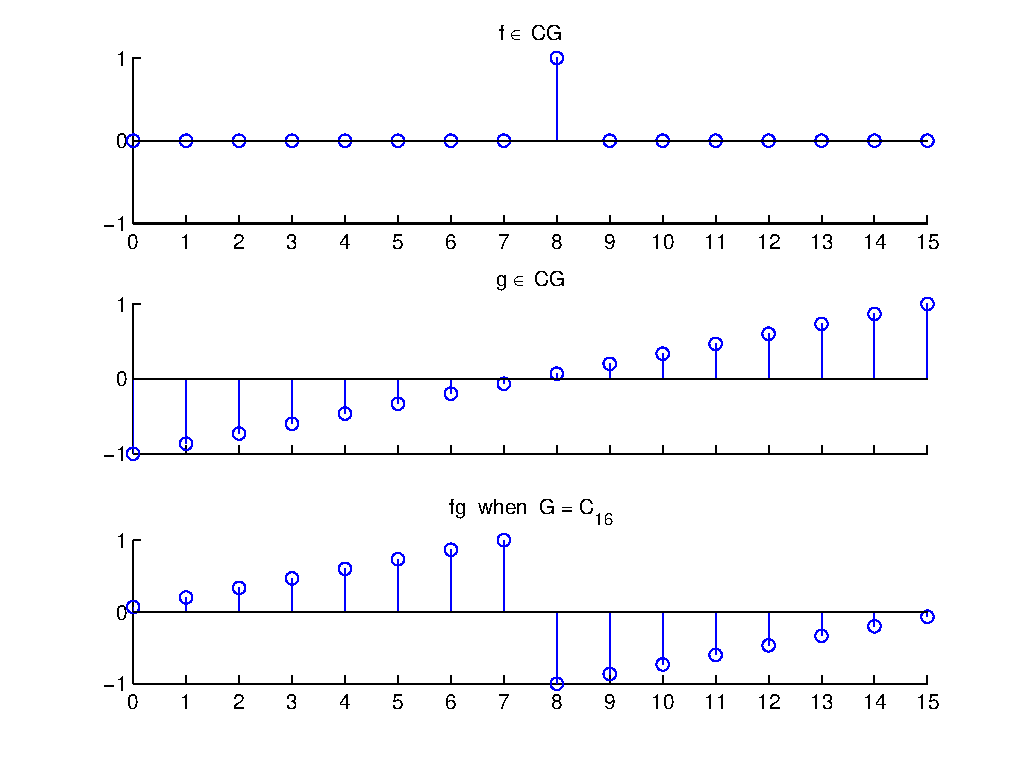
\includegraphics[width=\columnwidth, height=75mm]{C16conv_1}}}
\caption{Convolution of two signals indexed by the abelian
  group $C_{16}$.}
\label{fig:C16conv}
\end{figure}

Fig.~\ref{fig:k7conv} shows the convolution $C(f)g = fg$,
where $f$ is an impulse at the 9th sample, with group index $k_7$, and
$g$ is a linearly increasing sequence of 16 numbers ranging
from -1 to 1; $g$ can be represented as a vector,
or as an element of the group algebra $\C(C_8 \sdp \{1, k_7\})$,
\[
g = \sum_{m=0}^7 \sum_{j=0}^1 g(x^mk_7^j) x^mk_7^j
\]
with coefficients $g(x^mk_7^j)$ taking the values given
in~(\ref{eq:gvec}); \ie 
\[
g(1)=-1, \, g(x)=-0.8\bar{6}, %\, g(x^2)=-0.7\bar{3},
\ldots, g(x^7)=-0.0\bar{6},
\]
\[
g(k_7)=0.0\bar{6}, \, g(x k_7)=0.2, \ldots, g(x^7 k_7) = 1.
\]

\begin{figure}
\centerline{\framebox{
	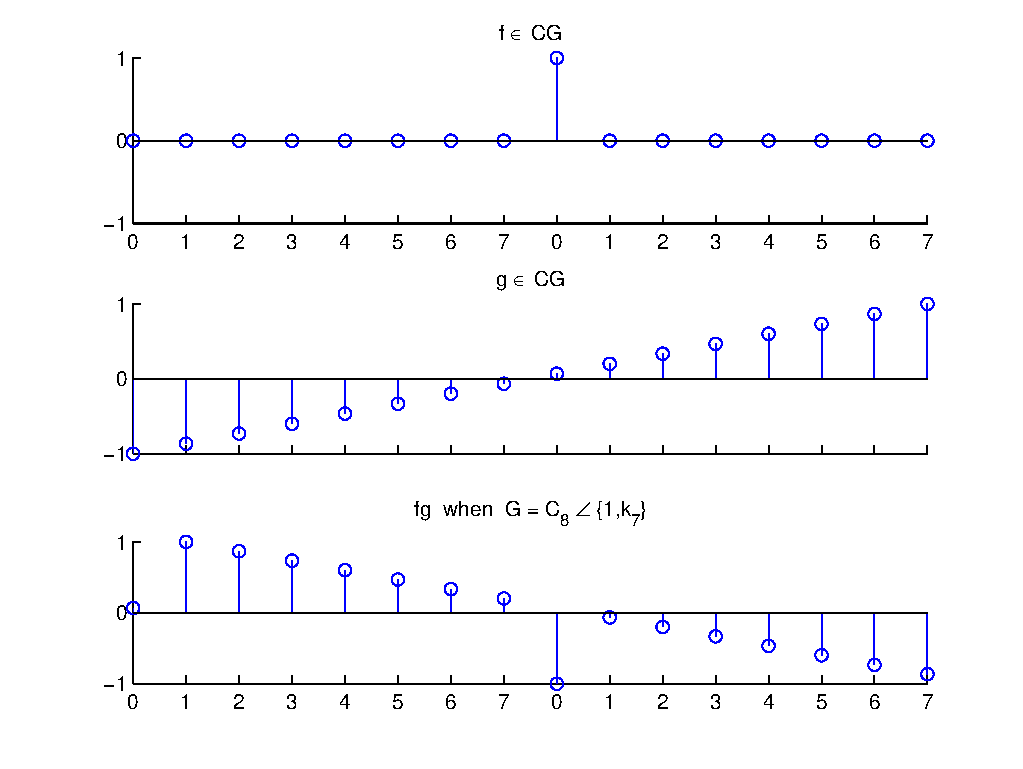
\includegraphics[width=\columnwidth, height=75mm]{k7conv_1}}}
\caption{The element $k_{N-1} \in G$ (top), where $N=8$ and $G = C_{8}\sdp \{1,k_7\}$ -- as an element of the group
  algebra, $f =  k_7 \in \CG$ is the ``impulse 
    function'' with one nonzero coefficient $f(k_7) =1$; 
    A linear signal $g\in \CG$ (middle); the product $fg = k_7g$ (bottom) is,
    in general, the convolution of $g$ by $f$, and is implemented
    by appealing to the convolution theorem and using a 
    generalized FFT algorithm.}
%\caption{Convolution of two signals indexed by the nonabelian
%  group $C_{8}\sdp \{1,k_7\}$.}
\label{fig:k7conv}
\end{figure}

\begin{figure}
\centerline{\framebox{
	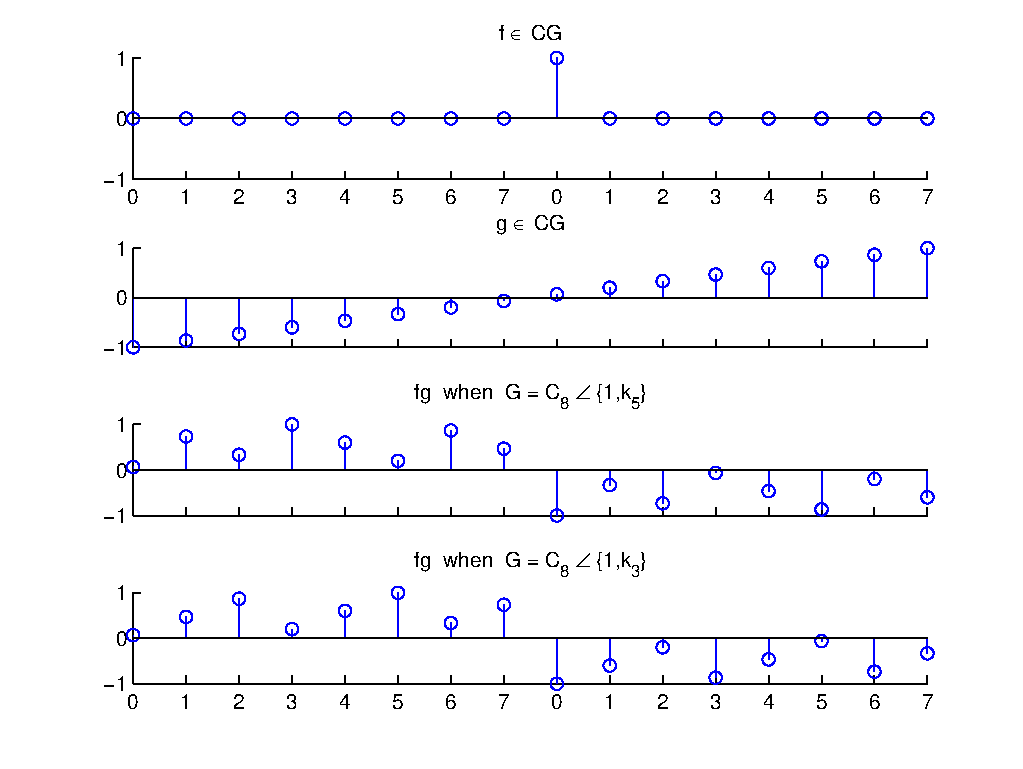
\includegraphics[width=\columnwidth, height=75mm]{k5_k3_conv_1}}}
\caption{Convolution of two signals indexed by the nonabelian
  groups $C_{8}\sdp \{1,k_5\}$ (third graph) and 
  $C_{8}\sdp \{1,k_5\}$ (fourth graph).}
\label{fig:k5_k3_conv}
\end{figure}


%=======================================================================
\subsection{Examples: 2-D Semidirect Product Indexing Sets}%\protect\footnotemark}
%=======================================================================
%\footnotetext{An and Tolimieri (2003), page 125.}
\begin{example}
Recall that $\lt{GL}(2,\Z/N)$ denotes the set of all $2\times 2$ invertible
matrices with coefficients in $\Z/N$.  
For $c\in \lt{GL}(2,\Z/N)$ such that $c^M$ is the identity,
%in $\lt{GL}(2,\Z/N)$ -- 
consider the \emph{action group} $K_c$ defined by
\[
C_M(k_c) = \{k_c^m : 0 \leq m < M\}, \quad
c = \begin{pmatrix} c_0 & c_1 \\ c_2 & c_3 \end{pmatrix}
%\in \lt{GL}(2,\Z/N).
\]
The semidirect product of $H$ and $K_c$ has elements
\[
H\varangle K_c = \{x^j y^k k_c^m : 0 \leq j,k < L, 0 \leq m< M\}
\]
and binary composition satisfying the following relations:
\[
x^L = y^L = k_c^M = 1,
\]
\[
x^{-1} = x^{L-1}, \quad y^{-1}= y^{L-1}, \quad k_c^{-1} = k_c^{M-1},
\]
\[
k_c x^j y^k = x^{c_0 j + c_1 k} y^{c_2 j + c_3 k} k_c.
\]
where the summands in the exponents are modulo $|H|=L$.
\end{example}

\subsection{Example: 2-D Rotations.} \textcolor{red}{\bf DEBUG this subsection.}\\

Let $A = C_N(x) \times C_N(y)$ with binary composition satisfying
\[
(x^my^j)(x^ny^k) = x^{m+n \bmod N}y^{j+k \bmod N},
\]
\[
%x^N = (x^N,1) = (1,1) = 1, \quad y^N = (1,y^N) = (1,1) = 1
x^N = y^N = 1, \quad x^{-1} = x^{N-1}, \quad y^{-1}= y^{N-1}.
\]
%\[x^{-1} = x^{N-1}, \quad y^{-1}= y^{N-1}.\]
Consider the action group $K_c$, $c\in \lt{GL}(2,\Z/N)$,
%\[c = \begin{pmatrix} c_0 & c_1 \\ c_2 & c_3 \end{pmatrix}.\]
with $c^M=1$.
%\ie $c^M = \begin{pmatrix} 1 & 0 \\ 0 & 1 \end{pmatrix}$.
%\ie \[\begin{pmatrix} c_0 & c_1 \\ c_2 & c_3 \end{pmatrix}^M
%= \begin{pmatrix} 1 & 0 \\ 0 & 1 \end{pmatrix}\]
The group generated by $k_c$ is the cyclic group of order
$M$ with elements $C_M(k_c) = \{k_c^m : 0 \leq m < M\}$.
Now suppose
\[
c(\theta) = \begin{pmatrix} \cos \theta \, &  -\sin \theta \\ 
                    \sin \theta \, & \, \cos \theta \end{pmatrix}.
\]
\begin{example}[Rotation by $\pi/2$]
The action group $K_{c(\pi/2)}$ has
\[
c(\pi/2) = \begin{pmatrix} 0\, & -1\\ 
                            1\, & \, 0 \end{pmatrix}.
\]
Since $c^4(\pi/2)$ is the identity, the group
has order $M=4$.
\end{example}

The semidirect product $A\varangle K_{c(\theta)}$ has elements
$\{x^j y^k k_{c(\theta)}^m : 0 \leq j,k < N,\, 0 \leq m < M\}$,
and binary composition satisfying
\[
x^N = y^N = k_{c(\theta)}^M = 1,
\]
\[
x^{-1} = x^{N-1}, \quad y^{-1}= y^{N-1}, \quad k_{c(\theta)}^{-1} = k_{c(\theta)}^{M-1},
\]
and
\[
k_{c(\theta)} x^j y^k = x^{j \cos \theta - k \sin \theta} y^{j \sin
  \theta + k \cos \theta} k_{c(\theta)},
\]
Additive operations in the exponents are modulo $|A|=N$.

We now demonstrate the effect of successive left
multiplications by the $k_c$ described above.  
%on an array representaion of an image $f$.  
Suppose an image $f$ has the following array representation:
{\footnotesize
\begin{equation*}
\left(
\begin{array}{cccc|cccc|cccc|cccc}
%\begin{array}{rrrr|rrrr|rrrr|rrrr}
0&0& 0  & 0 & 0 & 0 & 0 & 0 & 0 & 0 & 0 & 0 & 0 & 0 & 0 & 0 \\ 
0&10& 12 & 2 & 0 & 1 & 1 & 1 & 0 & 2 & 2 & 2 & 0 & 3 & 3 & 3 \\ 
0&9& 0  & 3 & 0 & 1 & 1 & 1 & 0 & 2 & 2 & 2 & 0 & 3 & 3 & 3 \\ 
0&8& 6  & 4 & 0 & 1 & 1 & 1 & 0 & 2 & 2 & 2 & 0 & 3 & 3 & 3 
\end{array}\right)
\end{equation*}
}
Notice that, in the left-most $4\times 4$ block of this
array, there is a $3\times 3$ subarray with entries
approximating the locations on the face of an analog clock.  
%These are the numbers on which we focus while left
%multiplication by $k_c$ transforms the entire array, 
%since they 
Such a configuration facilitate our observation of the local
behavior of the non-abelian group translation -- that is,
the action of $k_c$ on the elements within the given
$4\times 4$ block.  The subarrays of the 
three other $4\times 4$ blocks are designed to reveal the
global effect of the non-abelian translation.  That is, they
demonstrate how the blocks shift around (though the
elements within each of these blocks undergo the same
transformation as those of the first block.)
%observe this intra-block behavior since the numbers are all the same.)

The following are the array representations of $k_c f, \, k_c^2 f$, and $k_c^3 f$, resp. 
{\footnotesize
\begin{equation*}
\left(
\begin{array}{cccc|cccc|cccc|cccc}
0 & 0 & 0 & 0 & 0 & 0  & 0 & 0 & 0 & 0 & 0 & 0 & 0 & 0 & 0 & 0 \\ 
0 & 3 & 3 & 3 & 0 & 2  & 3 & 4 & 0 & 1 & 1 & 1 & 0 & 2 & 2 & 2 \\ 
0 & 3 & 3 & 3 & 0 & 12 & 0 & 6 & 0 & 1 & 1 & 1 & 0 & 2 & 2 & 2 \\ 
0 & 3 & 3 & 3 & 0 & 10 & 9 & 8 & 0 & 1 & 1 & 1 & 0 & 2 & 2 & 2 
\end{array}\right)
\end{equation*}
\begin{equation*}
\left(
\begin{array}{cccc|cccc|cccc|cccc}
0 & 0 & 0 & 0 & 0 & 0 & 0 & 0 & 0 & 0 & 0  & 0  & 0 & 0 & 0 & 0 \\ 
0 & 2 & 2 & 2 & 0 & 3 & 3 & 3 & 0 & 4 & 6  & 8  & 0 & 1 & 1 & 1 \\ 
0 & 2 & 2 & 2 & 0 & 3 & 3 & 3 & 0 & 3 & 0  & 9  & 0 & 1 & 1 & 1 \\ 
0 & 2 & 2 & 2 & 0 & 3 & 3 & 3 & 0 & 2 & 12 & 10 & 0 & 1 & 1 & 1 
\end{array}\right)
\end{equation*}
\begin{equation*}
\left(
\begin{array}{cccc|cccc|cccc|cccc}
0 & 0 & 0 & 0 & 0 & 0 & 0 & 0 & 0 & 0 & 0 & 0 & 0 & 0 & 0 & 0 \\ 
0 & 1 & 1 & 1 & 0 & 2 & 2 & 2 & 0 & 3 & 3 & 3 & 0 & 8 & 9 & 10 \\ 
0 & 1 & 1 & 1 & 0 & 2 & 2 & 2 & 0 & 3 & 3 & 3 & 0 & 6 & 0 & 12 \\ 
0 & 1 & 1 & 1 & 0 & 2 & 2 & 2 & 0 & 3 & 3 & 3 & 0 & 4 & 3 & 2 
\end{array}\right)
\end{equation*}
}

\subsection{Digital lines}
\textcolor{red}{\bf DEBUG this subsection.}\\
This section defines digital lines and the Matlab
routines used to process them. Such examples are useful
for demonstrating the nature of the generalized
translations and convolutions that are possible when 
the groups used to index the data are nonabelian.

\begin{figure}[t]               
%  \ifthenelse{\boolean{nofigures}}{}{
    \centering  
    \includegraphics[width=\columnwidth]{fline1}
%  }
  \caption{{\it Figures 10.4.1--10.4.3 of An (2003),
      re-produced with {\tt fline.m} program.}}  
  \label{fig:10.4.1}
\end{figure}

\begin{figure}[t]
%  \ifthenelse{\boolean{nofigures}}{}{
    \centering  
    \includegraphics[width=\columnwidth]{fline2}
%  }
    \caption{{\it Figures 10.4.4--10.4.6 of An (2003)
        re-produced with {\tt fline.m} program.}}  
  %% (see figures 10.4.4--10.4.6 in An & Tolimieri, pages 216--218)
  \label{fig:10.4.4}
\end{figure}

\begin{figure}
    \centering  
    \includegraphics[width=\columnwidth]{1234trans}
  \caption{Translates of an image in 
  $(C_N(x)\times C_N(y)) \sdp (K_a \times K_b)$.} 
  \label{fig:1234trans}
\end{figure}


%\begin{figure}[t]               
%%  \ifthenelse{\boolean{nofigures}}{}{
%    \centering  
%    \includegraphics[width=100mm]{1234trans}
%%  }
%  \caption{{\it Translates of an image in $G_1$.}}
%  \label{fig:1234trans}
%\end{figure}






%\verb!\input{Appendix/hafg}!
%\input{Appendix/hafg}
%\verb!\input{hafg/old/notation}!
%\input{hafg/old/notation}
%\verb!\input{hafg/old/nonabelianDSP}!
%\input{hafg/old/nonabelianDSP}
%\verb!\input{hafg/old/sdp}!
%\input{hafg/old/sdp}
%\verb!\input{hafg/old/examples}!
%\input{hafg/old/examples}
%\verb!\input{hafg/old/summary}!

% Reminder: the "draftcls" or "draftclsnofoot", not "draft", class option
% should be used if it is desired that the figures are to be displayed while
% in draft mode.

% An example of a floating figure using the graphicx package.
% Note that \label must occur AFTER (or within) \caption.
% For figures, \caption should occur after the \includegraphics.
%
%\begin{figure}
%\centering
%\includegraphics[width=2.5in]{myfigure}
% where an .eps filename suffix will be assumed under latex, 
% and a .pdf suffix will be assumed for pdflatex
%\caption{Simulation Results}
%\label{fig_sim}
%\end{figure}


% An example of a double column floating figure using two subfigures.
% (The subfigure.sty package must be loaded for this to work.)
% The subfigure \label commands are set within each subfigure command, the
% \label for the overall fgure must come after \caption.
% \hfil must be used as a separator to get equal spacing
%
%\begin{figure*}
%\centerline{\subfigure[Case I]{\includegraphics[width=2.5in]{subfigcase1}
% where an .eps filename suffix will be assumed under latex, 
% and a .pdf suffix will be assumed for pdflatex
%\label{fig_first_case}}
%\hfil
%\subfigure[Case II]{\includegraphics[width=2.5in]{subfigcase2}
% where an .eps filename suffix will be assumed under latex, 
% and a .pdf suffix will be assumed for pdflatex
%\label{fig_second_case}}}
%\caption{Simulation results}
%\label{fig_sim}
%\end{figure*}



% An example of a floating table. Note that, for IEEE style tables, the 
% \caption command should come BEFORE the table. Table text will default to
% \footnotesize as IEEE normally uses this smaller font for tables.
% The \label must come after \caption as always.
%
%\begin{table}
%% increase table row spacing, adjust to taste
%\renewcommand{\arraystretch}{1.3}
%\caption{An Example of a Table}
%\label{table_example}
%\centering
%% Some packages, such as MDW tools, offer better commands for making tables
%% than the plain LaTeX2e tabular which is used here.
%\begin{tabular}{|c||c|}
%\hline
%One & Two\\
%\hline
%Three & Four\\
%\hline
%\end{tabular}
%\end{table}

%
% \input{hafg/old/summary}
!
% This is the master examples.tex file -- the most
% up-to-date -- the one on which all others are based.
%
% ICMC2005-examples.tex was integrated on 2005.03.16.
% UHEE616-examples.tex was integrated on 2005.03.16.
% hafg-examples.tex was integrated on 2005.03.16.

%=======================================================================
\subsection{Examples: 1-D Semidirect Product Indexing Sets}
%\protect\footnotemark}
%=======================================================================
%\footnotetext{An and Tolimieri (2003), page 125.}
As seen above, when varying group structures are placed on indexing sets,
and products in the resulting group algebra are computed, 
interesting signal transforms obtain.  In this section,
we elucidate the nature of these operations by
examining some simple, concrete examples in detail.

Recall, in the notation 
%of (\ref{eq:cyclicGroup}) and (\ref{eq:unitGroup}) 
defined above,
%\begin{theorem}
the mapping $\Psi: U(N) \to Aut(C_N(x))$ is a group
isomorphism.
%\end{theorem}
Under this identification, we can form $C_N(x)\sdp K$
for any subgroup $K$ of $U(N)$.  A typical point in 
$C_N(x)\sdp K$ is denoted 
$(x^n, u), \, 0\leq n<N,\, u\in K$ with multiplication given
by  
\[
(x^m, u)(x^n, v) = (x^{m+un},uv), \quad 
0\leq m, n < N,\, u, v \in K
\]
where $m+un$ is taken modulo $N$.
We often use $k_u$ to denote the element $u\in K$ as this
avoids confusion that can arise at various places.

\begin{example}\protect\hspace{-1mm}\footnotemark
\footnotetext{An and Tolimieri (2003), page 125.}
\label{ex:g2}
Let $G_1$ be the abelian group 
\begin{equation}
G_1 = C_{2N}(x) = \{x^n : 0 \leq n < 2N\}. % = \{1, x, x^2, \ldots, x^{2N-1}\}
\end{equation}
Let $G_2$ be the \emph{dihedral group} %$\vs{D}_{2N}(x, k_{N-1})$,
%and suppose the elements of $G_2$ are indexed as follows:
with elements
\begin{eqnarray*}
G_2&=& C_N(x) \sdp \{1, k_{N-1}\}\\
&=& \{x^n k_{N-1}^j : 0 \leq n < N, 0 \leq j < 2\}.
\end{eqnarray*}
We order the elements of $G_2$ as follows:
\[
\{1, x, \ldots, x^{N-1}, k_{N-1}, xk_{N-1}, \ldots, x^{N-1}
k_{N-1}\}
\]
Thus, $G_2$ is divided into two blocks with $N$-samples per block.
\end{example}

\begin{example}\label{ex:g3}
Another group, $G_3$, will be constructed as follows: for some 
integer $M \geq 2$, define $N= 2^M$, so that
$\left(\frac{N}{2} + 1\right)^2 \equiv 1 \mod N$,
and $N/2 + 1$ generates a subgroup of $U(N)$ of order 2.
Let 
\begin{eqnarray*}
G_3 &=& C_N(x) \sdp \{1, k_{\frac{N}{2} + 1}\}\\
& =& \{x^n k_{\frac{N}{2}+1}^j : 0 \leq n < N, 0 \leq j < 2\}.
\end{eqnarray*}
Note that $G_2$ and $G_3$ are isomorphic groups.
\end{example}

{\bf Example {\ref{ex:g2}} (cont.)}  
By describing the translations of functions in $\CG_2$,  
we will see that the nonabelian translates of
$\CG_2$ are ``intra-block time-reversal'' operations.
A similar analysis of $G_3$ shows that the nonabelian 
translates of $\CG_3$ perform an ``intra-block interleave''
operation. 

Multiplication on $G_2$ obeys the following relations:
\begin{equation}\label{eq:id0}
  x^N = k_{N-1}^2 = 1,
\end{equation}
\begin{equation}
  x^mk_{N-1}^{j+1} \; x^nk_{N-1}^j = 
  \begin{cases} 
    x^{m-n}, & j=0,\\
    x^{m+n}, & j=1.
  \end{cases}
\end{equation}
If $z=x^mk_{N-1}$, then $z^2=1$, thus $\inverse{z}=z$.

For $f\in \CG_2$, 
\begin{equation}\label{eq:f}
  f = \sum_n f(x^n)x^n + f(x^n k_{N-1})x^n k_{N-1}.
\end{equation}
By~(\ref{eq:id0}), the nonabelian translate $k_{N-1}f$
is given by
\[
\sum_n f(k_{N-1}x^n)x^n + f(k_{N-1}x^n k_{N-1})x^n k_{N-1}
\]
which is equivalent to 
%  &=& \sum_n f(x^{(N-1)n} k_{N-1})x^n + f(x^{(N-1)n}) x^n k_{N-1},\nonumber\\
\begin{equation}\label{eq:natran}
\sum_n f(x^{N-n} k_{N-1})x^n + f(x^{N-n}) x^n k_{N-1}.
\end{equation}
Comparing (\ref{eq:f}) and (\ref{eq:natran}), we see that
the nonabelian translate of $f\in \CG_2$ swaps the first $N$
samples of $f$ with the remaining $N$ samples, and performs
a time-reversal within each sub-block.


%
% Integrated additional content from ICMC2005-examples.tex here
%
%For a simple linear function, this special translation is
%illustrated in Fig.~\ref{fig:G2trans}.

To express this another way, define $h=k_{N-1}f$. 
The first $N$ coefficients of $h$ are defined in terms of $f$ as
\[
h(x^n)= f(x^{N-n} k_{N-1}), \quad 0\leq n < N,
\]
while the remaining $N$ coefficients are given by
\[
h(x^n k_{N-1}) = f(x^{N-n}), \quad 0\leq n < N.
\]
For a simple linear function, this special translation is
illustrated in Fig.~\ref{fig:k7conv}.

%\begin{figure}
%\centerline{\epsfig{figure=figures/G2transV,width=80mm, height=55mm}}
%\caption{{\small {\it A linear signal $f\in \CG_2$, where $N
%    = 8$ (left); the element $k_{N-1} \in G_2$ (middle) --
%    as an element of the group algebra, $k_{N-1}$ is the ``impulse
%    function'' $g \in \CG_2$ with one nonzero coefficient,
%    $g(k_{N-1}) =1$; the product $gf = k_{N-1}f$ (right) is,
%    in general, the convolution product and is implemented
%    by appealing to the convolution theorem and using a 
%    generalized FFT algorithm.}}}
%    \label{fig:G2trans}
%\end{figure}

A similar analysis of $G_3 = C_N(x) \sdp \{1,
k_{\frac{N}{2} + 1}\}$ reveals
that the nonabelian translates of $\CG_3$ interleave the 
elements within each $N$-sample sub-block of $G_3$, 
in addition to swapping the two blocks.
This is illustrated in Fig.~\ref{fig:k5_k3_conv}.

\subsection{A Few Generalized Convolutions Computed}
%Convolutions on Different Groups Computed}

Fig.~\ref{fig:C16conv} illustrates a cyclic
convolution of two discrete signals, with 16 samples each, 
indexed with the abelian group $C_{16}$. 
The first graph in Fig.~\ref{fig:C16conv} is a graph of the
signal $f$, which is simply an impulse at the 9th sample; \ie
$f(x^8) = 1$ and 
$f(x^m) = 0, \, m\neq 8$.
The second signal, $g$, appears in the middle graph of
Fig.~\ref{fig:C16conv}.  A linearly increasing sequence
of 16 numbers ranging from -1 to 1, $g$ can be represented
as a vector of values
\begin{equation}
  \label{eq:gvec}
\mathbf{g} = 
%\begin{pmatrix}
(-1, \, -0.8\bar{6}, \, -0.7\bar{3}, \ldots,
%-0.6, \, -0.4\bar{6} \\ -0.\bar{3} \\  -0.2 \\  -0.0\bar{6} \\ 0.0\bar{6} \\ 0.2
%\\ 0.\bar{3} \\ 0.4\bar{6} \\ 0.6 \\ 
0.7\bar{3}, \, 0.8\bar{6}, \, 1)
%\end{pmatrix}
\end{equation}
or as an element of the group algebra $\C C_{16}$,
\[
g = \sum_{m=0}^{15} g(x^m) x^m,
\]
where the coefficients $g(x^m)$ take the values given
in~(\ref{eq:gvec}).  The third graph in
Fig.~\ref{fig:C16conv} shows the result of the convolution
$C(f)g = fg$.    Evidently, when signals are indexed by
elements of the abelian group $C_{16}$, then the product $fg$
is the familiar cyclic convolution of $f$ and $g$. (Recall,
convolution by an impulse effects a translation.)

\begin{figure}
\centerline{\framebox{
	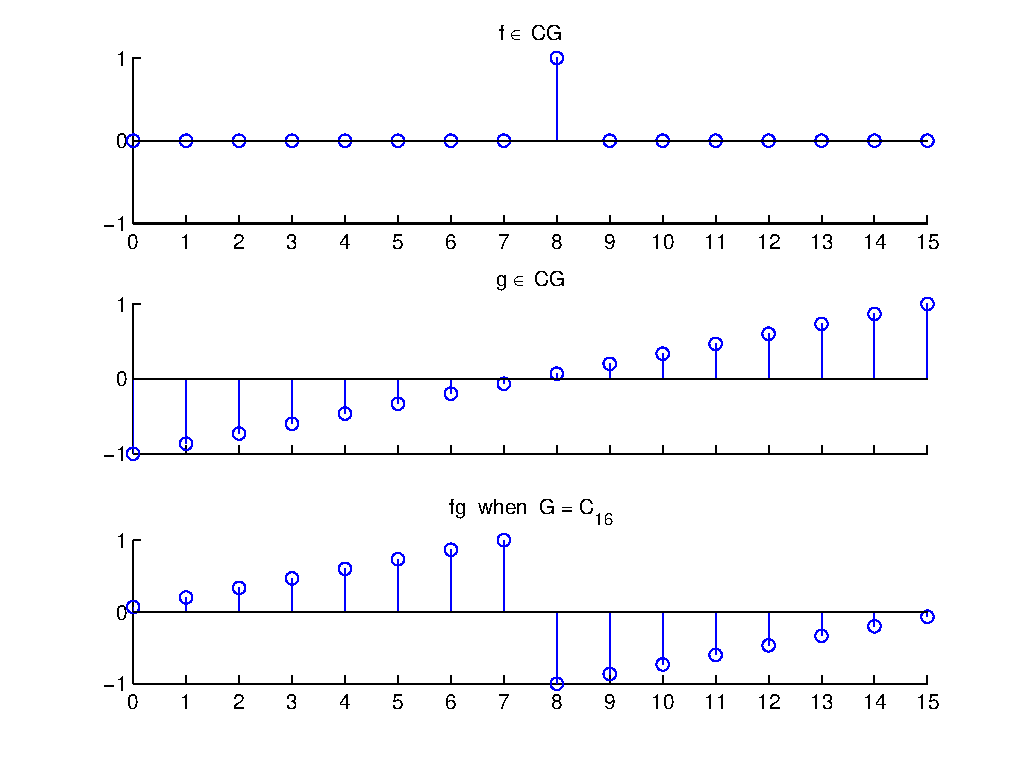
\includegraphics[width=\columnwidth, height=75mm]{C16conv_1}}}
\caption{Convolution of two signals indexed by the abelian
  group $C_{16}$.}
\label{fig:C16conv}
\end{figure}

Fig.~\ref{fig:k7conv} shows the convolution $C(f)g = fg$,
where $f$ is an impulse at the 9th sample, with group index $k_7$, and
$g$ is a linearly increasing sequence of 16 numbers ranging
from -1 to 1; $g$ can be represented as a vector,
or as an element of the group algebra $\C(C_8 \sdp \{1, k_7\})$,
\[
g = \sum_{m=0}^7 \sum_{j=0}^1 g(x^mk_7^j) x^mk_7^j
\]
with coefficients $g(x^mk_7^j)$ taking the values given
in~(\ref{eq:gvec}); \ie 
\[
g(1)=-1, \, g(x)=-0.8\bar{6}, %\, g(x^2)=-0.7\bar{3},
\ldots, g(x^7)=-0.0\bar{6},
\]
\[
g(k_7)=0.0\bar{6}, \, g(x k_7)=0.2, \ldots, g(x^7 k_7) = 1.
\]

\begin{figure}
\centerline{\framebox{
	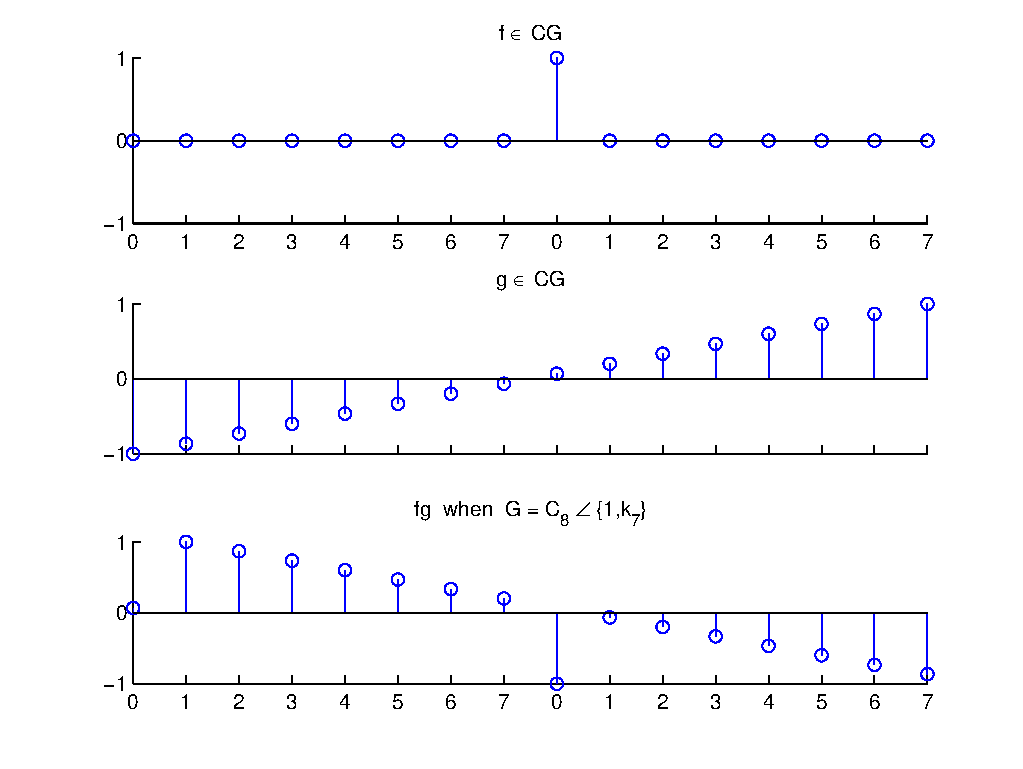
\includegraphics[width=\columnwidth, height=75mm]{k7conv_1}}}
\caption{The element $k_{N-1} \in G$ (top), where $N=8$ and $G = C_{8}\sdp \{1,k_7\}$ -- as an element of the group
  algebra, $f =  k_7 \in \CG$ is the ``impulse 
    function'' with one nonzero coefficient $f(k_7) =1$; 
    A linear signal $g\in \CG$ (middle); the product $fg = k_7g$ (bottom) is,
    in general, the convolution of $g$ by $f$, and is implemented
    by appealing to the convolution theorem and using a 
    generalized FFT algorithm.}
%\caption{Convolution of two signals indexed by the nonabelian
%  group $C_{8}\sdp \{1,k_7\}$.}
\label{fig:k7conv}
\end{figure}

\begin{figure}
\centerline{\framebox{
	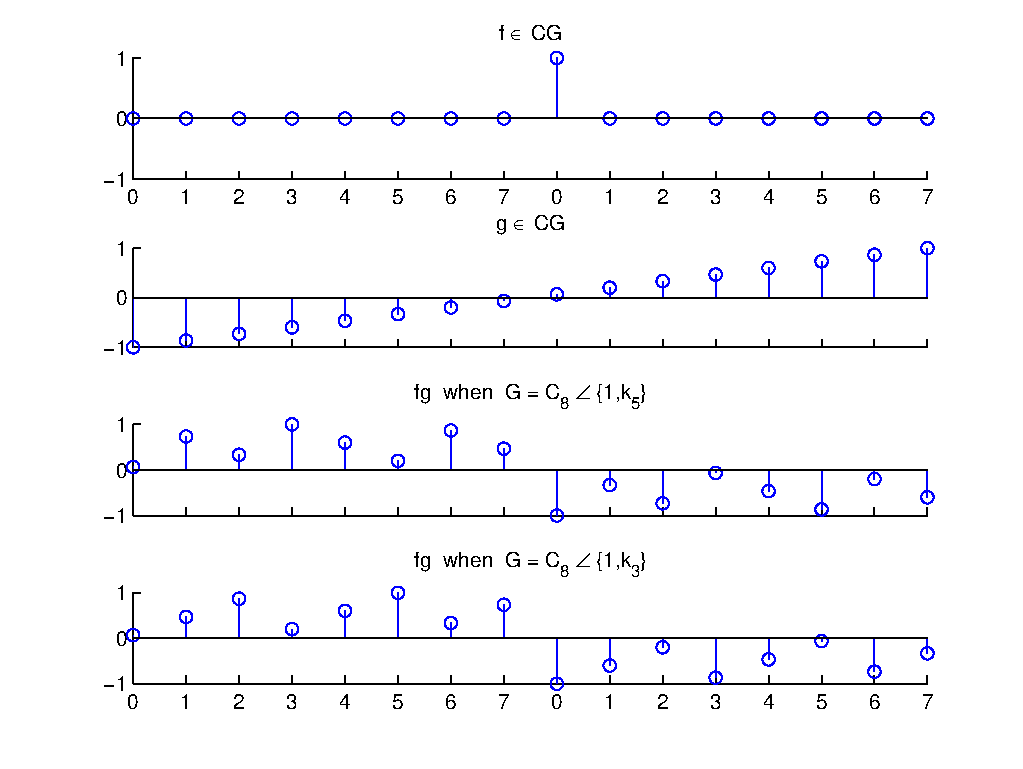
\includegraphics[width=\columnwidth, height=75mm]{k5_k3_conv_1}}}
\caption{Convolution of two signals indexed by the nonabelian
  groups $C_{8}\sdp \{1,k_5\}$ (third graph) and 
  $C_{8}\sdp \{1,k_5\}$ (fourth graph).}
\label{fig:k5_k3_conv}
\end{figure}


%=======================================================================
\subsection{Examples: 2-D Semidirect Product Indexing Sets}%\protect\footnotemark}
%=======================================================================
%\footnotetext{An and Tolimieri (2003), page 125.}
\begin{example}
Recall that $\lt{GL}(2,\Z/N)$ denotes the set of all $2\times 2$ invertible
matrices with coefficients in $\Z/N$.  
For $c\in \lt{GL}(2,\Z/N)$ such that $c^M$ is the identity,
%in $\lt{GL}(2,\Z/N)$ -- 
consider the \emph{action group} $K_c$ defined by
\[
C_M(k_c) = \{k_c^m : 0 \leq m < M\}, \quad
c = \begin{pmatrix} c_0 & c_1 \\ c_2 & c_3 \end{pmatrix}
%\in \lt{GL}(2,\Z/N).
\]
The semidirect product of $H$ and $K_c$ has elements
\[
H\varangle K_c = \{x^j y^k k_c^m : 0 \leq j,k < L, 0 \leq m< M\}
\]
and binary composition satisfying the following relations:
\[
x^L = y^L = k_c^M = 1,
\]
\[
x^{-1} = x^{L-1}, \quad y^{-1}= y^{L-1}, \quad k_c^{-1} = k_c^{M-1},
\]
\[
k_c x^j y^k = x^{c_0 j + c_1 k} y^{c_2 j + c_3 k} k_c.
\]
where the summands in the exponents are modulo $|H|=L$.
\end{example}

\subsection{Example: 2-D Rotations.} \textcolor{red}{\bf DEBUG this subsection.}\\

Let $A = C_N(x) \times C_N(y)$ with binary composition satisfying
\[
(x^my^j)(x^ny^k) = x^{m+n \bmod N}y^{j+k \bmod N},
\]
\[
%x^N = (x^N,1) = (1,1) = 1, \quad y^N = (1,y^N) = (1,1) = 1
x^N = y^N = 1, \quad x^{-1} = x^{N-1}, \quad y^{-1}= y^{N-1}.
\]
%\[x^{-1} = x^{N-1}, \quad y^{-1}= y^{N-1}.\]
Consider the action group $K_c$, $c\in \lt{GL}(2,\Z/N)$,
%\[c = \begin{pmatrix} c_0 & c_1 \\ c_2 & c_3 \end{pmatrix}.\]
with $c^M=1$.
%\ie $c^M = \begin{pmatrix} 1 & 0 \\ 0 & 1 \end{pmatrix}$.
%\ie \[\begin{pmatrix} c_0 & c_1 \\ c_2 & c_3 \end{pmatrix}^M
%= \begin{pmatrix} 1 & 0 \\ 0 & 1 \end{pmatrix}\]
The group generated by $k_c$ is the cyclic group of order
$M$ with elements $C_M(k_c) = \{k_c^m : 0 \leq m < M\}$.
Now suppose
\[
c(\theta) = \begin{pmatrix} \cos \theta \, &  -\sin \theta \\ 
                    \sin \theta \, & \, \cos \theta \end{pmatrix}.
\]
\begin{example}[Rotation by $\pi/2$]
The action group $K_{c(\pi/2)}$ has
\[
c(\pi/2) = \begin{pmatrix} 0\, & -1\\ 
                            1\, & \, 0 \end{pmatrix}.
\]
Since $c^4(\pi/2)$ is the identity, the group
has order $M=4$.
\end{example}

The semidirect product $A\varangle K_{c(\theta)}$ has elements
$\{x^j y^k k_{c(\theta)}^m : 0 \leq j,k < N,\, 0 \leq m < M\}$,
and binary composition satisfying
\[
x^N = y^N = k_{c(\theta)}^M = 1,
\]
\[
x^{-1} = x^{N-1}, \quad y^{-1}= y^{N-1}, \quad k_{c(\theta)}^{-1} = k_{c(\theta)}^{M-1},
\]
and
\[
k_{c(\theta)} x^j y^k = x^{j \cos \theta - k \sin \theta} y^{j \sin
  \theta + k \cos \theta} k_{c(\theta)},
\]
Additive operations in the exponents are modulo $|A|=N$.

We now demonstrate the effect of successive left
multiplications by the $k_c$ described above.  
%on an array representaion of an image $f$.  
Suppose an image $f$ has the following array representation:
{\footnotesize
\begin{equation*}
\left(
\begin{array}{cccc|cccc|cccc|cccc}
%\begin{array}{rrrr|rrrr|rrrr|rrrr}
0&0& 0  & 0 & 0 & 0 & 0 & 0 & 0 & 0 & 0 & 0 & 0 & 0 & 0 & 0 \\ 
0&10& 12 & 2 & 0 & 1 & 1 & 1 & 0 & 2 & 2 & 2 & 0 & 3 & 3 & 3 \\ 
0&9& 0  & 3 & 0 & 1 & 1 & 1 & 0 & 2 & 2 & 2 & 0 & 3 & 3 & 3 \\ 
0&8& 6  & 4 & 0 & 1 & 1 & 1 & 0 & 2 & 2 & 2 & 0 & 3 & 3 & 3 
\end{array}\right)
\end{equation*}
}
Notice that, in the left-most $4\times 4$ block of this
array, there is a $3\times 3$ subarray with entries
approximating the locations on the face of an analog clock.  
%These are the numbers on which we focus while left
%multiplication by $k_c$ transforms the entire array, 
%since they 
Such a configuration facilitate our observation of the local
behavior of the non-abelian group translation -- that is,
the action of $k_c$ on the elements within the given
$4\times 4$ block.  The subarrays of the 
three other $4\times 4$ blocks are designed to reveal the
global effect of the non-abelian translation.  That is, they
demonstrate how the blocks shift around (though the
elements within each of these blocks undergo the same
transformation as those of the first block.)
%observe this intra-block behavior since the numbers are all the same.)

The following are the array representations of $k_c f, \, k_c^2 f$, and $k_c^3 f$, resp. 
{\footnotesize
\begin{equation*}
\left(
\begin{array}{cccc|cccc|cccc|cccc}
0 & 0 & 0 & 0 & 0 & 0  & 0 & 0 & 0 & 0 & 0 & 0 & 0 & 0 & 0 & 0 \\ 
0 & 3 & 3 & 3 & 0 & 2  & 3 & 4 & 0 & 1 & 1 & 1 & 0 & 2 & 2 & 2 \\ 
0 & 3 & 3 & 3 & 0 & 12 & 0 & 6 & 0 & 1 & 1 & 1 & 0 & 2 & 2 & 2 \\ 
0 & 3 & 3 & 3 & 0 & 10 & 9 & 8 & 0 & 1 & 1 & 1 & 0 & 2 & 2 & 2 
\end{array}\right)
\end{equation*}
\begin{equation*}
\left(
\begin{array}{cccc|cccc|cccc|cccc}
0 & 0 & 0 & 0 & 0 & 0 & 0 & 0 & 0 & 0 & 0  & 0  & 0 & 0 & 0 & 0 \\ 
0 & 2 & 2 & 2 & 0 & 3 & 3 & 3 & 0 & 4 & 6  & 8  & 0 & 1 & 1 & 1 \\ 
0 & 2 & 2 & 2 & 0 & 3 & 3 & 3 & 0 & 3 & 0  & 9  & 0 & 1 & 1 & 1 \\ 
0 & 2 & 2 & 2 & 0 & 3 & 3 & 3 & 0 & 2 & 12 & 10 & 0 & 1 & 1 & 1 
\end{array}\right)
\end{equation*}
\begin{equation*}
\left(
\begin{array}{cccc|cccc|cccc|cccc}
0 & 0 & 0 & 0 & 0 & 0 & 0 & 0 & 0 & 0 & 0 & 0 & 0 & 0 & 0 & 0 \\ 
0 & 1 & 1 & 1 & 0 & 2 & 2 & 2 & 0 & 3 & 3 & 3 & 0 & 8 & 9 & 10 \\ 
0 & 1 & 1 & 1 & 0 & 2 & 2 & 2 & 0 & 3 & 3 & 3 & 0 & 6 & 0 & 12 \\ 
0 & 1 & 1 & 1 & 0 & 2 & 2 & 2 & 0 & 3 & 3 & 3 & 0 & 4 & 3 & 2 
\end{array}\right)
\end{equation*}
}

\subsection{Digital lines}
\textcolor{red}{\bf DEBUG this subsection.}\\
This section defines digital lines and the Matlab
routines used to process them. Such examples are useful
for demonstrating the nature of the generalized
translations and convolutions that are possible when 
the groups used to index the data are nonabelian.

\begin{figure}[t]               
%  \ifthenelse{\boolean{nofigures}}{}{
    \centering  
    \includegraphics[width=\columnwidth]{fline1}
%  }
  \caption{{\it Figures 10.4.1--10.4.3 of An (2003),
      re-produced with {\tt fline.m} program.}}  
  \label{fig:10.4.1}
\end{figure}

\begin{figure}[t]
%  \ifthenelse{\boolean{nofigures}}{}{
    \centering  
    \includegraphics[width=\columnwidth]{fline2}
%  }
    \caption{{\it Figures 10.4.4--10.4.6 of An (2003)
        re-produced with {\tt fline.m} program.}}  
  %% (see figures 10.4.4--10.4.6 in An & Tolimieri, pages 216--218)
  \label{fig:10.4.4}
\end{figure}

\begin{figure}
    \centering  
    \includegraphics[width=\columnwidth]{1234trans}
  \caption{Translates of an image in 
  $(C_N(x)\times C_N(y)) \sdp (K_a \times K_b)$.} 
  \label{fig:1234trans}
\end{figure}


%\begin{figure}[t]               
%%  \ifthenelse{\boolean{nofigures}}{}{
%    \centering  
%    \includegraphics[width=100mm]{1234trans}
%%  }
%  \caption{{\it Translates of an image in $G_1$.}}
%  \label{fig:1234trans}
%\end{figure}






%\verb!\input{Appendix/hafg}!
%\input{Appendix/hafg}
%\verb!\input{hafg/old/notation}!
%\input{hafg/old/notation}
%\verb!\input{hafg/old/nonabelianDSP}!
%\input{hafg/old/nonabelianDSP}
%\verb!\input{hafg/old/sdp}!
%\input{hafg/old/sdp}
%\verb!\input{hafg/old/examples}!
%\input{hafg/old/examples}
%\verb!\input{hafg/old/summary}!

% Reminder: the "draftcls" or "draftclsnofoot", not "draft", class option
% should be used if it is desired that the figures are to be displayed while
% in draft mode.

% An example of a floating figure using the graphicx package.
% Note that \label must occur AFTER (or within) \caption.
% For figures, \caption should occur after the \includegraphics.
%
%\begin{figure}
%\centering
%\includegraphics[width=2.5in]{myfigure}
% where an .eps filename suffix will be assumed under latex, 
% and a .pdf suffix will be assumed for pdflatex
%\caption{Simulation Results}
%\label{fig_sim}
%\end{figure}


% An example of a double column floating figure using two subfigures.
% (The subfigure.sty package must be loaded for this to work.)
% The subfigure \label commands are set within each subfigure command, the
% \label for the overall fgure must come after \caption.
% \hfil must be used as a separator to get equal spacing
%
%\begin{figure*}
%\centerline{\subfigure[Case I]{\includegraphics[width=2.5in]{subfigcase1}
% where an .eps filename suffix will be assumed under latex, 
% and a .pdf suffix will be assumed for pdflatex
%\label{fig_first_case}}
%\hfil
%\subfigure[Case II]{\includegraphics[width=2.5in]{subfigcase2}
% where an .eps filename suffix will be assumed under latex, 
% and a .pdf suffix will be assumed for pdflatex
%\label{fig_second_case}}}
%\caption{Simulation results}
%\label{fig_sim}
%\end{figure*}



% An example of a floating table. Note that, for IEEE style tables, the 
% \caption command should come BEFORE the table. Table text will default to
% \footnotesize as IEEE normally uses this smaller font for tables.
% The \label must come after \caption as always.
%
%\begin{table}
%% increase table row spacing, adjust to taste
%\renewcommand{\arraystretch}{1.3}
%\caption{An Example of a Table}
%\label{table_example}
%\centering
%% Some packages, such as MDW tools, offer better commands for making tables
%% than the plain LaTeX2e tabular which is used here.
%\begin{tabular}{|c||c|}
%\hline
%One & Two\\
%\hline
%Three & Four\\
%\hline
%\end{tabular}
%\end{table}

%
% \input{hafg/old/summary}


%--SUMMARY-----------------------------------------------------------------
%\verb!\input{DSP/isma2004-summary}!
%\input{DSP/isma2004-summary}

%\verb!\input{DSP/isma2004-summary-long}!
%\input{DSP/isma2004-summary-long}

\verb!%
\section{Summary and Conclusions}
Basic DSP theory was reviewed with a focus on 
\emph{translation invariance} -- translation invariant
operators of $\LG$, and translation invariant
subspaces of $\LG$. 
When such great significance is attached to translation invariance, 
a deeper understanding of exponential functions, and their 
unrivaled status in classical DSP, is possible.  
In particular, exponentials are the \emph{characters} 
of abelian group indexing sets, such as $\Z/N$, over which
classical DSP is performed.  
Each character of an abelian group represents a one-dimensional
translation invariant subspace, and the characters are eigenvectors
of translations, therefore, of convolutions. 
%(which explains why expansions in the character basis -- \eg
%classical Fourier transform -- diagonalize the convolution
%product).  

We described the group algebra $\CG$,
the algebra isomorphism $\LG \simeq \CG$, and why it is
useful for manipulations involving (generalized)
translations and convolutions of the space of signals. 
We saw that, for an abelian group $A$, translations of $\LA$
represent simple linear shifts in space or time, while for a nonabelian
group $G$, translations of $\LG$ are more general than
simple spatial or temporal shifts.  This leads to
more interesting translation invariant subspaces.

Motivating many studies in the area of noncommutative
harmonic analysis (including this one) is a simple
but important fact about the generalized translations that
result when a signal is indexed by a nonabelian group.
As we have seen, such operations offer more complex and
interesting signal transformations.  Equally important,
however, is the fact that each transformation can be written
as a left-multiplication. Thus, the increase in signal transform
complexity resulting from a nonabelian indexing scheme
comes at no increase in computational complexity. 


% if have a single appendix:
%\appendix[Proof of the Zonklar Equations]
% or
%\appendix  % for no appendix heading
% do not use \section anymore after \appendix, only \section*
% is possibly needed

% use appendices with more than one appendix
% then use \section to start each appendix
% you must declare a \section before using any
% \subsection or using \label (\appendices by itself
% starts a section numbered zero.)
%
% Use this command to get the appendices' numbers in "A", "B" instead of the
% default capitalized Roman numerals ("I", "II", etc.).
% However, the capital letter form may result in awkward subsection numbers
% (such as "A-A"). Capitalized Roman numerals are the default.
%\useRomanappendicesfalse
%
%\appendices
%\section{Proof of the First Zonklar Equation}
%Appendix one text goes here.

% you can choose not to have a title for an appendix
% if you want by leaving the argument blank
%\section{}
%Appendix two text goes here.

% use section* for acknowledgement
\section*{Acknowledgment}
% optional entry into table of contents (if used)
%\addcontentsline{toc}{section}{Acknowledgment}
The author would like to thank Textron Systems and the U.S.~Navy
for supporting this research.  This work also owes a great deal to Myoung
An and Richard Tolimieri, whose prior contributions to this field are
responsible for anything of value in the present work. The author thanks them
for many helpful conversations and suggestions, but takes full responsibility for any
errors that appear above.
!
%
\section{Summary and Conclusions}
Basic DSP theory was reviewed with a focus on 
\emph{translation invariance} -- translation invariant
operators of $\LG$, and translation invariant
subspaces of $\LG$. 
When such great significance is attached to translation invariance, 
a deeper understanding of exponential functions, and their 
unrivaled status in classical DSP, is possible.  
In particular, exponentials are the \emph{characters} 
of abelian group indexing sets, such as $\Z/N$, over which
classical DSP is performed.  
Each character of an abelian group represents a one-dimensional
translation invariant subspace, and the characters are eigenvectors
of translations, therefore, of convolutions. 
%(which explains why expansions in the character basis -- \eg
%classical Fourier transform -- diagonalize the convolution
%product).  

We described the group algebra $\CG$,
the algebra isomorphism $\LG \simeq \CG$, and why it is
useful for manipulations involving (generalized)
translations and convolutions of the space of signals. 
We saw that, for an abelian group $A$, translations of $\LA$
represent simple linear shifts in space or time, while for a nonabelian
group $G$, translations of $\LG$ are more general than
simple spatial or temporal shifts.  This leads to
more interesting translation invariant subspaces.

Motivating many studies in the area of noncommutative
harmonic analysis (including this one) is a simple
but important fact about the generalized translations that
result when a signal is indexed by a nonabelian group.
As we have seen, such operations offer more complex and
interesting signal transformations.  Equally important,
however, is the fact that each transformation can be written
as a left-multiplication. Thus, the increase in signal transform
complexity resulting from a nonabelian indexing scheme
comes at no increase in computational complexity. 


% if have a single appendix:
%\appendix[Proof of the Zonklar Equations]
% or
%\appendix  % for no appendix heading
% do not use \section anymore after \appendix, only \section*
% is possibly needed

% use appendices with more than one appendix
% then use \section to start each appendix
% you must declare a \section before using any
% \subsection or using \label (\appendices by itself
% starts a section numbered zero.)
%
% Use this command to get the appendices' numbers in "A", "B" instead of the
% default capitalized Roman numerals ("I", "II", etc.).
% However, the capital letter form may result in awkward subsection numbers
% (such as "A-A"). Capitalized Roman numerals are the default.
%\useRomanappendicesfalse
%
%\appendices
%\section{Proof of the First Zonklar Equation}
%Appendix one text goes here.

% you can choose not to have a title for an appendix
% if you want by leaving the argument blank
%\section{}
%Appendix two text goes here.

% use section* for acknowledgement
\section*{Acknowledgment}
% optional entry into table of contents (if used)
%\addcontentsline{toc}{section}{Acknowledgment}
The author would like to thank Textron Systems and the U.S.~Navy
for supporting this research.  This work also owes a great deal to Myoung
An and Richard Tolimieri, whose prior contributions to this field are
responsible for anything of value in the present work. The author thanks them
for many helpful conversations and suggestions, but takes full responsibility for any
errors that appear above.


%-----------------------------------------------------------------------------
\bibliographystyle{IEEEtran}
%\bibliographystyle{ieeetr}
%\begin{thebibliography}{10}
\bibliography{wjd}
%\bibitem[1]{An:2003} An, M. and Tolimieri, R, ``Group Filters and Image
%Processing,'' Psypher Press, 2003. $<$http://www.psypher.net$>$.
%\end{thebibliography}
%-----------------------------------------------------------------------------
\end{document}
